\documentclass[12pt]{article}
\usepackage[utf8]{inputenc}
\usepackage[english]{babel}
\usepackage[a4paper, portrait, margin=1.2in]{geometry}
\usepackage{fancyhdr,lipsum}
\usepackage{graphicx}
\usepackage{xcolor}
\usepackage{enumitem}
\usepackage{hyperref}
\usepackage[font=footnotesize,labelfont=bf]{caption}
\usepackage{amsmath}
\usepackage{fancyvrb}
\usepackage{moreverb}

\pagestyle{fancy} 
\fancyhf{} 
\fancyhead[L]{Andrea Giarduz}
\fancyhead[R]{Design Document -- DIMA}
\fancyhead[C]{Veronica Grosso}
\fancyfoot[C]{\thepage}

\title{DIMA -- DD}
\author{Veronica Grosso \and Andrea Giarduz}

\begin{document}

\begin{titlepage}
    \begin{center}
        \vspace*{1cm}
        \begin{figure}[h]
            \begin{center}
                
\includegraphics[width=4.5cm, clip]{../../assets/logo.png}
            \end{center}
            \label{title:logo}
        \end{figure}
        \vspace*{1cm}
        \LARGE{{\scshape Politecnico di Milano}}
        \\
        \LARGE{Design and Implementation of Mobile Applications}
        \\
        \LARGE{2021/2022}

        \vspace*{1.5cm}
        \Huge{DD}
        \\
        \Large{{\scshape Design Document}}

        \vspace{1.5cm}

        \LARGE{\textbf{SubscribeME -- a subscription manager app}}
        \\
        \vspace{1cm}
        \Large{August 30, 2022}
        \vfill

        \Large{Giarduz Andrea\\
            Grosso Veronica
        }

        \vspace{0.8cm}

        \Large
        Prof. Luciano Baresi
    \end{center}
\end{titlepage}
\tableofcontents

\newpage
\begin{center}
    \LARGE{\textbf{SubscribeME Design Document}}
\end{center}
\section{Introduction}\label{sec:intro}
\subsection{Purpose}
The purpose of this Design Document is to provide a guide and a walk-through of the application \textit{SubscribeME}, in order to explain the design choices we made and to show the logic behind its architecture.

\subsection{Scope}
\textit{SubscribeME} is a mobile application that keeps track of all the memberships that the user activated. The users should be aware of how much money they are spending and in which subscriptions, and be reminded of each renewal date.

In this way, the users are always in control of their finances, without forgetting where their money is going, when the payment is due and whether the specific subscription is worth keeping.

\subsection{Document Structure}
The document is structured in eight sections:
\begin{enumerate}
    \item[\ref{sec:intro}.] \textbf{Introduction}: is an overview of the purpose of the Design Document and of the problem analyzed.
    \item[\ref{sec:features}.] \textbf{Application Features}: presents the application features and the basic functioning of the application.
    \item[\ref{sec:char}.] \textbf{User Characteristics}: explains the user characteristics and use cases adopted when the app was realized. It gives an overview of the target population that was considered during the design phase.
    \item[ \ref{sec:design}.] \textbf{Design Overview}: the system architecture is presented. Diagrams and graphs are used to help the reader visualize and understand the underlying structure and to see how the different components are linked to each other and work together. The implementation of the server-client architecture is explained.
    \item[\ref{sec:ui}.] \textbf{User Interface Design}: User Interface choices and designs, along with screenshots of the final implementation of the app.
    \item[\ref{sec:test}.] \textbf{Implementation, Integration and Test Plan}: testing of the components and the results and statistics of these tests are presented analytically.
    \item[\ref{sec:dev}.] \textbf{Future Development}: the next steps of this project occupy the last part of the document, Section , giving a few inputs on possible future works that can be implemented.
    \item[\ref{sec:ref}.] \textbf{References}: includes the tools and the references used to define the document.
\end{enumerate}

\section{Application Features}\label{sec:features}
There are five main features in the \textit{SubscribeME} app:
\begin{itemize}
    \item the \textbf{Login/Signup} function: the users need to signup and login to be able to use the application. There is a persistent layer for each user and all the information is saved in the Data Base.
    \item the \textbf{Home page}: a sum-up is provided, with the amount of money that the user is spending at that moment on subscriptions. There is also the reminder to pay for the memberships with the closest deadline.
    \item the \textbf{Subscriptions List}: the user should be able to add, modify and delete their subscriptions on the app.
          In order to add a membership, the user must provide the following details:
          \begin{itemize}
              \item[-] the name of the membership,
              \item[-] the date when they subscribed to the plan,
              \item[-] how often does the subscription activates,
              \item[-] the amount of money due,
              \item[-] which card is being currently used to pay for it,
              \item[-] whether the payment is automatic or not,
              \item[-] if they are sharing the subscription with any friends.
          \end{itemize}
          In this last case, the user knows they owe money to a friend, even if the subscription may not be in their name. In particular, if the user is not the `owner' of the subscription, they cannot edit it, but only withdraw from the offer.
    \item the \textbf{Statistics page}: offers them the opportunity of analyzing first hand their expenses, seeing how many subscriptions per category (Music, Movies \& TV, Shopping, Tech or Other) they activated and how much money they spend on each of them.
    \item the \textbf{Profile section}: it contains the Friends list and the feature to add new friends. Also there are some settings.
\end{itemize}

\newpage
\section{User Characteristics}\label{sec:char}
The target population is anyone who has multiple subscriptions active at the same time, who wants some help in keeping track of the costs and of the deadlines. Most importantly, it is useful for people who tend to activate memberships and then forget about them, so that they do not waste any money in unused perks.

\subsection{Use case Diagram}
Figure \ref{fig:usecase} shows the use case diagram from the point of view of the typical user. Every action can be performed only upon registration and, the following times, upon login. The available features involve handling the subscriptions, visualize the statistics and future deadlines and to manage friends.

Going into further detail, a subscription must be added in order to be able to modify it, delete it and to see the related statistics and future deadlines.

\noindent Concerning the management of friends, they can be added providing the friend's registration e-mail. The second user can then accept the request or deny it; once accepted, the friend can also be removed.

\begin{figure}[h]
    \begin{center}
        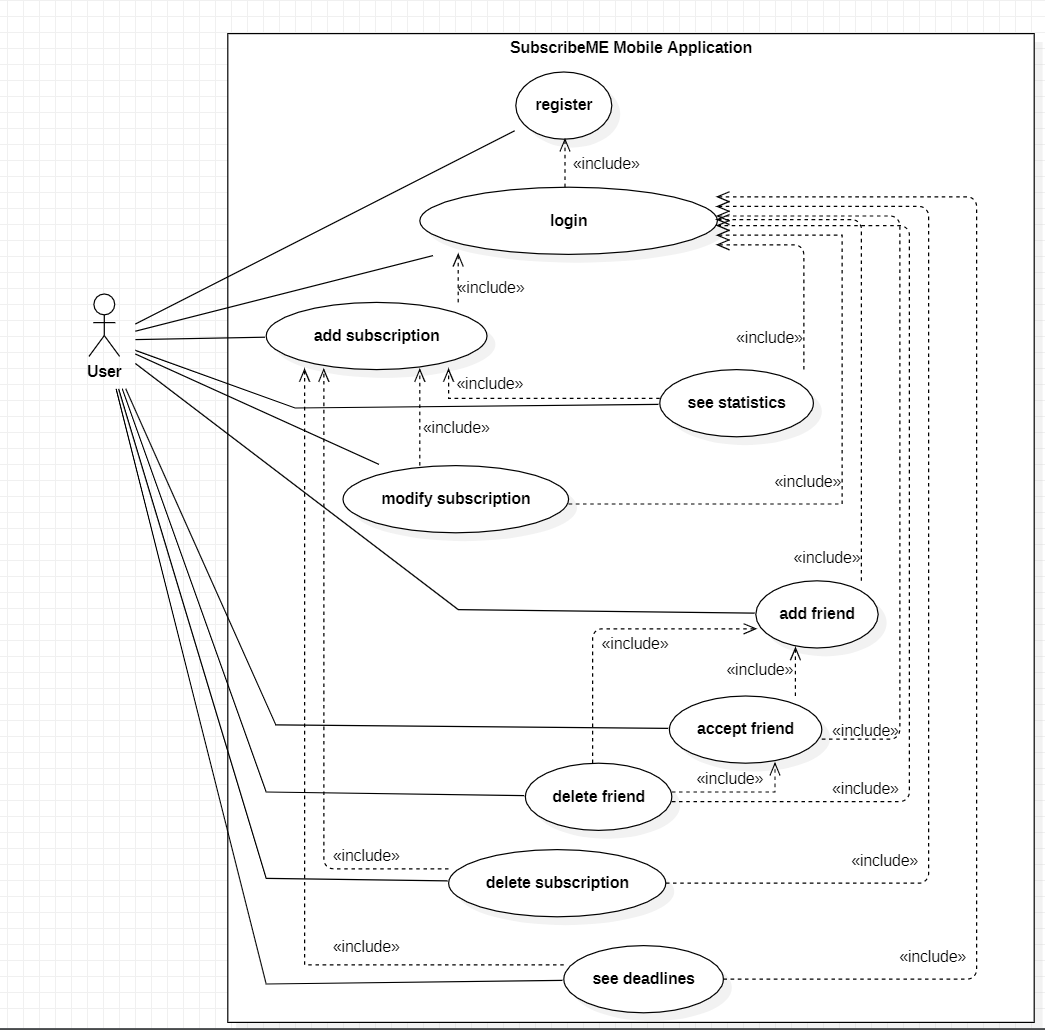
\includegraphics[width=0.9\textwidth, trim={0 0.1cm 0 0.2cm},, clip]{../../assets/usecaseDiagram.PNG}
    \end{center}
    \caption{Use Case diagram}
    \label{fig:usecase}
\end{figure}

\subsection{Scenarios}\label{sub:scenarios}
\subsubsection{Reminder of the payment for a subscription}
Arya activated a monthly Apple plan, as an additional warranty for her devices. She wants to be sure to be covered, because these devices are fundamental for her job. She is also very busy and she can get distracted, so she uploaded the information about this subscription on \textit{SubscribeME} and then totally forgot. Luckily, at the time of the renewal of the offer, she sees on the app that she needs to pay for the plan.

\subsubsection{Keeping track of the subscriptions}
John loves subscribing for every free-trial he puts his eyes on. He cannot miss any opportunities. He often registers with all of his personal and card information. He receives a notification from the bank, his account is empty: he check the billing transcript and he realizes that he had forgotten to unsubscribe from the trials and he has been paying for months for offers he did not even use. He now wants to keep track of every subscription he activates, so he downloads \textit{SubscribeME} to help him monitor his memberships and finances.

\subsubsection{Monitoring the Statistics}
Mary is a university student and is on a budget, since she does not have a job yet. With the recent price increases and inflation, she cannot afford to waste any money. That is why she decides to use \textit{SubscribeME}: she adds all of her subscriptions, she goes to the `Statistics' page and she realizes that she is definitely spending much more than she was aware of. The majority of her subscriptions are for `Movies \& TV': she does not need all of them.

\subsubsection{Share a subscription}
Amber and Luc are twins and they want to activate the Spotify family plan, to split the money of the subscription. However, Amber does not trust Luc to be honest with her about the price and to keep his end of the deal, so they both use \textit{SubscribeME} in order to keep track of the deadlines and the money that they are spending. Both see the information about the plan and can monitor it.

\newpage
\section{Design Overview}\label{sec:design}
\subsection{Architectural Design Overview}
The \textit{SubscribeMe} application is based on the client-server paradigm. The user connects via the mobile app (the client) to the services provided in the server, such as the application logic (backend) and the database. Overall, the implementation structure can be described as a \textbf{Model-View-Controller} pattern. On one hand, the client contains the View and some input verification (part of the Controller); the server, on the other hand, has additional checks (the rest of the Controller) and the whole application Model.

The platform employed to implement the server architecture is Google Firebase, an out-of-the-box solution to manage the backend, as well as all the authentication functions and the data storage (Firestore).

\noindent In order to keep an updated and coherent state of the whole application, the Redux Toolkit library has been used. The Toolkit version is the latest release of the Redux code and it is meant to simplify and shorten the Redux configuration and code.

\begin{figure}[h]
    \begin{center}
        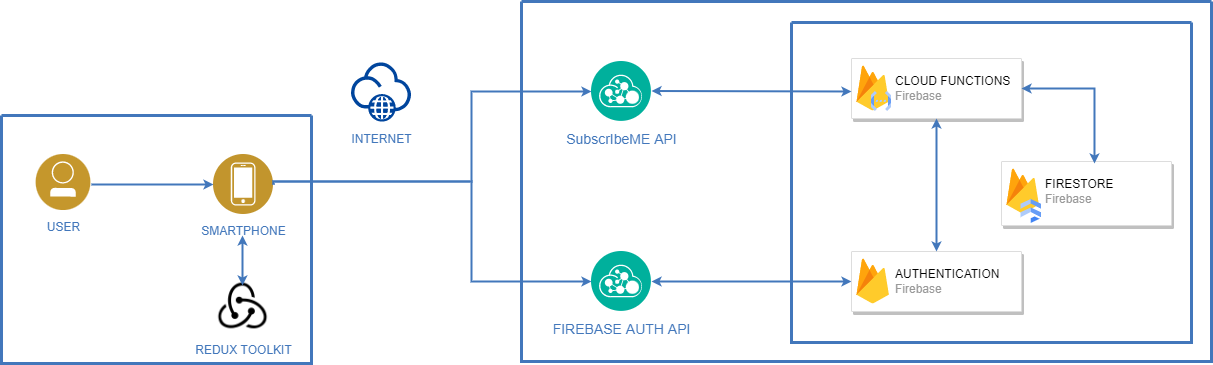
\includegraphics[width=\textwidth, clip]{../../assets/highLevel.png}
    \end{center}
    \caption{High Level Architecture Diagram}
    \label{fig:highLevel}
\end{figure}

In Figure \ref{fig:highLevel}, it is possible to better understand the structure of the entire application.
The application on the user's device interacts directly with Redux Toolkit and, through internet, with the application own APIs and the Firebase Authentication API. The former has access to the Cloud Functions stored in Firebase, while the latter uses the Authentication Functions from the Firebase own authentication provider. The Cloud Functions need access to the data stored in the Firestore database.

\subsection{Client Application}
The technology used to implement the application is \textbf{React Native}. This allowed a faster, cleaner and, most of all, single code base that can at the same time render an iOS and an Android app. The framework uses JavaScript as underlying programming language.

The client side contains mainly the View of the MVC pattern. Its structure is presented in Figure \ref{fig:navigationTree} and in is divided in two main branches, in order to keep every domain separated from the others and allow the user to better navigate from one section to the other, both logically and physically in the frontend implementation.

In particular, the `main application', as stated in Figure \ref{fig:navigationTree}, is implemented as a bottom tabular navigation, for a fast switch from page to page. The other links are stack navigation links, one for each domain, so that the history of one stack does not influence or negatively impacts the other stacks.

\begin{figure}[h!]
    \begin{center}
        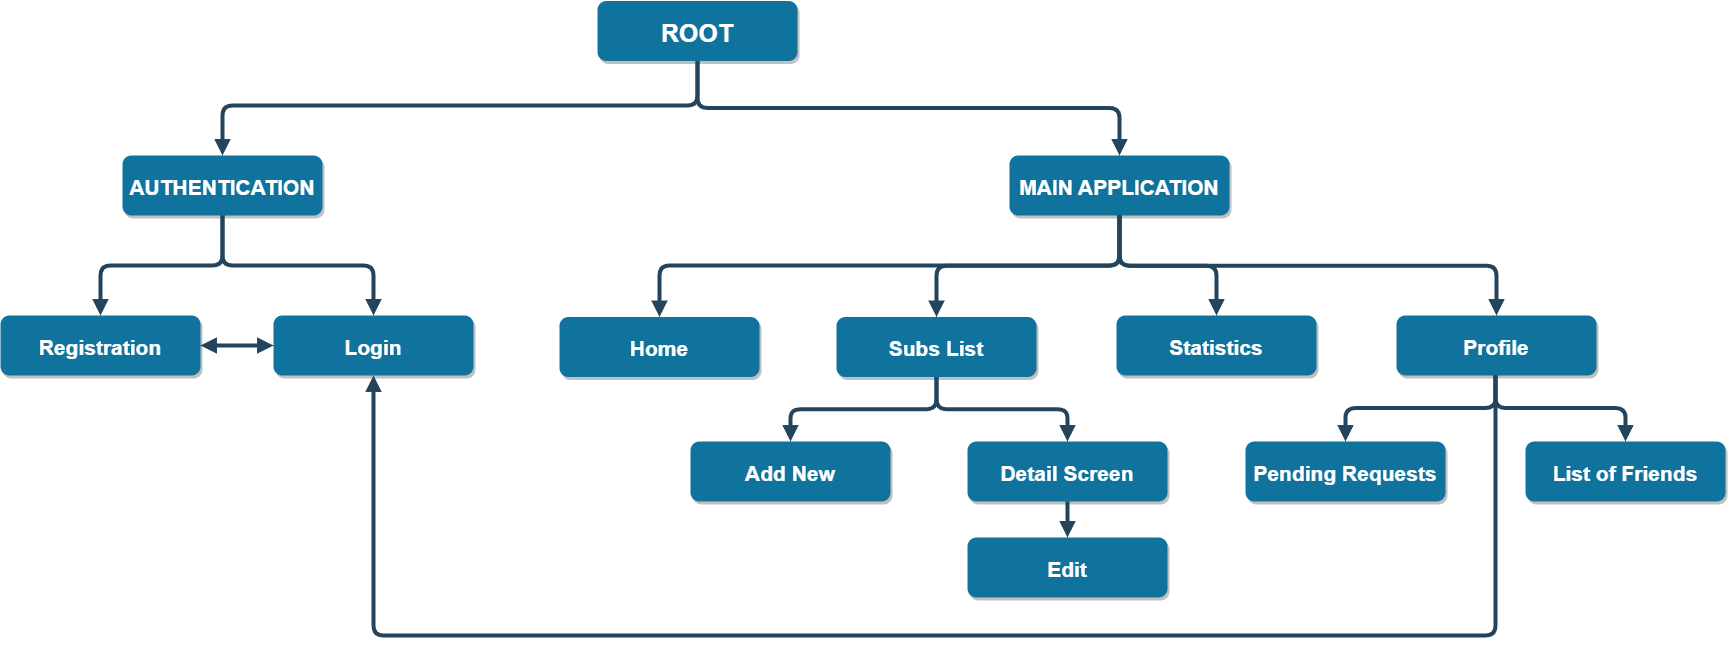
\includegraphics[width=\textwidth, clip]{../../assets/navigationTree.drawio.png}
    \end{center}
    \caption{Application Navigation Tree: the structure of all the pages the user can navigate to.}
    \label{fig:navigationTree}
\end{figure}

\subsubsection{Application Pages}
{\scshape{Home Screen}}
\vspace{0.2cm}

\noindent The Home Screen's function is to summarize the useful data that the user can later analyze more in detail in other sections. Specifically, there is a greeting message and two boxes that display: \begin{itemize}
    \item the \textbf{financial} information: how much money the user is spending a year/a month and how many subscriptions they subscribed to;
    \item the \textbf{payment reminders}: which are the next two subscriptions that need to be renewed and payed and in how many days.
\end{itemize}

\vspace{0.5cm}
\noindent{\scshape{Subscription List Screen}}
\vspace{0.2cm}

\noindent The Subscription List Screen shows two separate lists of plans: \begin{itemize}
    \item `My Subscriptions': are all of the offers that the users activated on their own behalf and, optionally, for other friends. They are the owners of the subscription and the only ones who can edit it.
    \item `Shared with me': vice versa, these are the plans that a friend activated and shared with the user. In this case, the only possible action is to delete the plan and to rescind the offer.
\end{itemize}

Clicking on the subscription item opens a Detail Page, where the user can review all the information about the membership. There is the possibility to remove it and possibly edit it (if the user is the owner).

At the bottom of the Subscription List Page there is a button `Add New'. This is for inserting in the database a new membership, and the form requires many fields to fill in all the data that can be useful to the user.

\vspace{0.5cm}
\noindent{\scshape{Statistics Screen}}
\vspace{0.2cm}

\noindent The Statistics Screen renders some graphs, in order to visualize the aggregated data about the memberships. The plans can be flagged with only one of the following categories:
\begin{itemize}
    \item[--] Movies \& TV,
    \item[--] Shopping,
    \item[--] Music,
    \item[--] Tech,
    \item[--] Other.
\end{itemize}

\noindent There are two main graphs: \begin{enumerate}
    \item `Your Category Shares': it is a pie chart to show the percentage of plans active in each category.
    \item `Money spent a month for each category': the sum of the money spent in each category thanks to an approximation computed on a monthly basis.
\end{enumerate}

\vspace{0.5cm}
\noindent{\scshape{Profile Page}}
\vspace{0.2cm}

\noindent The Profile Page provides some settings, both in friends and profile management: \begin{itemize}
    \item `Manage Friends':
          \begin{itemize}
              \item `Add a friend': provides the basic instructions to add a friend (by inserting the friend's e-mail)
              \item `Pending Requests': allows the navigation to a new page, that shows all the requests not yet accepted nor rejected, both in the Inbox and Sent.
              \item `List of Friends': shows in a new screen the list of friends and allows the user to delete them.
          \end{itemize}
    \item `Profile Settings': editable account information
          \begin{itemize}
              \item `Name': the account name, used for friends to easily recognize each other (non-unique information);
              \item `E-mail': unique identifier, can be changed upon insertion of the profile password;
              \item `Password': profile password necessary for the login, can be changed upon correct insertion of the old one.
          \end{itemize}
\end{itemize}

A `Logout' button brings the user back to the authentication page.

\subsubsection{Component Diagram}
The \textit{SubscribeME} application component diagram is pictured in Figure \ref{fig:componentGen}. It illustrates the `Root' components, alias the main application screens and how the Root communicates with Redux Toolkit and with the Cloud Functions. To avoid confusion, internal links from the single components to the Root interfaces are omitted.

Other diagrams are not shown, due to their trivial structure and linear flow (e.g. login and registration pages).

\begin{figure}[h!]
    \begin{center}
        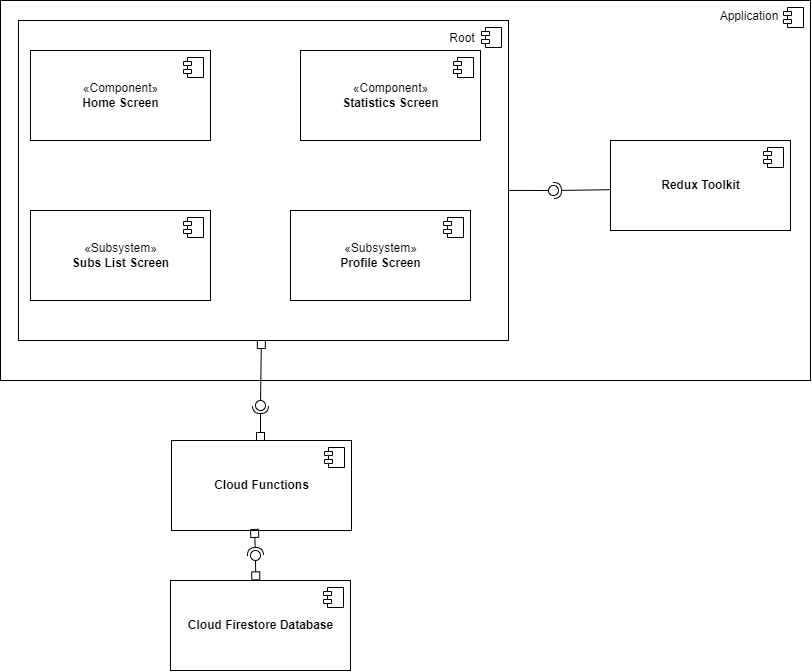
\includegraphics[width=0.65\textwidth, clip]{../../assets/generalComponent.drawio.png}
    \end{center}
    \caption{General component diagram for the mobile application.}
    \label{fig:componentGen}
\end{figure}
\vspace{0.5cm}

\subsection{Firebase}
The application requires \textbf{authentication} to be used, so that the application can properly store each individual's memberships and details. There is also some sensible data, such as the card's last four digits, so it is recommended to register with a strong password. Indeed, there is a `Password Strength Bar' that helps the user realize whether the typed password is good enough for them.

The authentication per se is handled with Google Firebase, which has a simple interface that allows to automatically manage the registration (with the verification e-mail) and, if needed, the password retrieval e-mail (with the link for a safe reset of the password). The registration requires a chosen name, the e-mail and a password. Firebase already checks that the information provided is compatible with the wanted data. Nevertheless, we implemented some \textbf{client-side input verifications} as well, in order to allow only:
\begin{enumerate}
    \item names with alpha-numeric values and less than ten characters. The name is not unique, but is used by friends to easily recognize each other when adding them to shared subscriptions. Since the same name can be used by different users, the e-mail may be shown as well, to avoid any ambiguity.
    \item e-mails correctly formatted;
    \item passwords with at least six characters.
\end{enumerate}

In order to improve the user's experience, the logged user will keep access in the future, with no need of further authentication every time he opens the application, thanks to the \textbf{Persistent Storage} of React Native. Only in case of manual logout, the user needs to access again through the login page. As expected, the user must reauthenticate before changing e-mail or password.

\subsection{Cloud Functions}
The Cloud Functions use node.js as language to express the backend logic.
They integrate flawlessly with the other services of the Firebase ecosystem. For instance, they offer a complete SDK to interact with the authentication and database products. They \textbf{abstract} the whole server infrastructure; the setup time and costs are perfectly suited for an application of this size, but they can also be easily scaled to handle a heavier workload.

Together with the authentication, they are the endpoints of the backend accessible by the application. They implement the logic of the application, and can be divided in two types of functions: \begin{itemize}
    \item \textbf{onCall} functions: triggered by events in the frontend.They encapsulate the authentication information of the user and possible input data. These ones are clearly the only Cloud functions accessible from the `outside', and thus happen through an HTTPS connection.
    \item \textbf{trigger} functions: functions that respond to precise events of the Firestore database and/or of the authentication services (e.g. creation of a user, deletion of a subscription). They are used to keep the backend data consistent at all times.
\end{itemize}

In our implementation, we exploit the authentication information included with each call, to manage and control accesses to the data only if the user is actually authorized to do so. For example, only the owner of a subscription can modify its data. Maliciously crafted requests would fail these checks and consequently would be rejected.

Furthermore, each response is in a JSON format, including message about the success of the requests and the required data. Specific \textbf{error messages} are associated to specific points of failure, in order to keep the user informed of the nature of the error, while also guiding the developers in solving any bug.

\subsubsection{\textit{SubscribeME} APIs}
The application APIs can be divided into four different categories: \begin{enumerate}
    \item manageSubscription (Figure \ref{fig:manageSub}): here there are all the functions which goal is to handle the subscriptions, such as retrieving all the subscriptions for a user, adding a plan, edit it or remove a subscription from a member who rescinded the offer.

    \item manageUser (Figure \ref{fig:manageUs}): the functions to handle the profile requests, for example to set a name, to send a friends request or to reply to a request.
    \item subscriptionMgmtTriggers (Figure \ref{fig:subtrigger}): trigger functions to keep the database updated (on deletion or edit of a subscription).
    \item userMgmtTriggers (Figure \ref{fig:usertrigger}): trigger function to allow the insertion of a new user into the database in a consistent manner, as a response to the events generated by the Authentication service.
\end{enumerate}

\begin{figure}[h!]
    \centering
    \begin{SaveVerbatim}{VerbCode}
        + getUserSubscription()
        + setNewSubscription(subscriptionInfo: Object{})
        + editSubscription(subscriptionInfo: Object{})
        + removeMember(subscription: String, userToRemove: String)
        + deleteSubscription(subscription: String)
    \end{SaveVerbatim}
    \setlength{\fboxsep}{5mm}
    \fbox{\BUseVerbatim{VerbCode}}
    \caption{manageSubscription functions}~\label{fig:manageSub}
\end{figure}

\begin{figure}[h!]
    \centering
    \begin{SaveVerbatim}{VerbCode}
        + setName(name: String)
        + addFriendRequest(email: String)
        + answerFriendRequest(friendUid: String, accepted: Boolean)
        + removeFriend(friendUid: String)
        + getFriendsData()
        + getCurrentUserInfo()
    \end{SaveVerbatim}
    \setlength{\fboxsep}{5mm}
    \fbox{\BUseVerbatim{VerbCode}}
    \caption{manageUser functions}~\label{fig:manageUs}
\end{figure}

\begin{figure}[h!]
    \centering
    \begin{SaveVerbatim}{VerbCode}
        + onSubDelete()
        + onSubEdited()
    \end{SaveVerbatim}
    \setlength{\fboxsep}{5mm}
    \fbox{\BUseVerbatim{VerbCode}}
    \caption{subscriptionMgmtTriggers functions}~\label{fig:subtrigger}
\end{figure}

\begin{figure}[h!]
    \centering
    \begin{SaveVerbatim}{VerbCode}
        + onUserCreation()
    \end{SaveVerbatim}
    \setlength{\fboxsep}{5mm}
    \fbox{\BUseVerbatim{VerbCode}}
    \caption{userMgmtTriggers function}~\label{fig:usertrigger}
\end{figure}


\subsection{Firestore database}
Cloud Firestore is a \textbf{NoSQL database} hosted on \textbf{cloud}, in particular Firebase's newest database for mobile app development. Compared to the old Realtime Database, it provides faster queries and better scaling. Even if both databases have client-first SDKs (no servers to deploy and maintain) and realtime updates, Cloud Firestore manages the data as a \textbf{collection of documents}, which are very similar to JSON files. Since \textit{SubscribeME} data have a pretty simple structure, this solution allows for a more agile and dynamic option.

Our Firestore configuration is set to be inaccessible from the `outside', by protecting the database from unauthorized requests: only the database admin is allowed to edit any data. It is possible to see that in Figure \ref{fig:rule}: this is the only rule present in the Firestore database and it states that the only acceptable requests are from the admins. This way, this becomes a \textbf{single point of failure} when considering unwanted access and simplifies the rule definition. Every function of manipulation of the saved data or retrieval of information must be from the `inside', through a Cloud Function.

\begin{figure}[h!]
    \begin{center}
        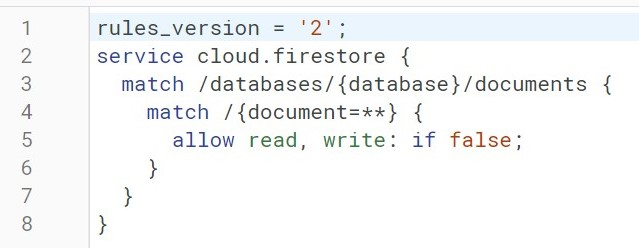
\includegraphics[width=0.6\textwidth, clip]{../../assets/firestoreRule.jpg}
    \end{center}
    \caption{Firestore rule for accepting requests.}
    \label{fig:rule}
\end{figure}

\subsubsection{Database Structure}
Given the Cloud Firestore structure as a collection of documents, we decided to store the data in two different collections: \begin{itemize}
    \item \texttt{subscriptions}: each documents, characterized by a unique identifier, contains: \begin{itemize}
              \item \texttt{autoRenewal:} if the payment automatically generates at the end of the renewal period;
              \item \texttt{card:} last four digits of the card used to pay;
              \item \texttt{category:} category of the subscription (used to render the background color as well);
              \item \texttt{currency:} payment currency;
              \item \texttt{customName:} manually inserted name of the subscription;
              \item \texttt{customType:} manually inserted type of the subscription;
              \item \texttt{members:} list of friends with whom the user is sharing the subscription;
              \item \texttt{name:} name of the subscription, chosen from a fixed list;
              \item \texttt{owner:} user who created the subscription;
              \item \texttt{price:} money due for the activation of the subscription;
              \item \texttt{renewalDate:} date when the user activated the subscription;
              \item \texttt{renewalPeriod:} length of repetition for the payment (e.g. week or month);
              \item \texttt{type:} type of the subscription, chosen from a fixed list (e.g. student plan or family plan).
          \end{itemize}
    \item \texttt{users}:  \begin{itemize}
              \item \texttt{friends:} list of friends added;
              \item \texttt{pendingFriendsRecv:} list of pending friend requests received;
              \item \texttt{pendingFriendsSent:} list of pending friend requests sent out;
              \item \texttt{subscriptions:} list of subscriptions activated for a user.
          \end{itemize}
\end{itemize}

This way, there can be repeated data (so the consistency in the database is harder to maintain), but it allows the management of faster and more complex queries.


\subsection{Redux Toolkit}
Redux Toolkit is the latest version of the Redux library. It has now become the standard way to write Redux logic and it overall simplifies the writing of Redux code, it speeds up development and provides good error catching, by managing the whole workflow.

More in detail, it keeps the \textbf{application state updated}, as a single point of truth for the whole application. Every page change updates in background the state, so that the user can get the correct data and enjoy an optimal experience at the same time. The strength of this library is represented by a \textbf{centralized} state: this is able to keep the data \textbf{coherent} throughout the different screens and pages.
Subscription and friends data are stored locally through Redux Toolkit, allowing the application to be accessible (of course with limited functionality) even in the event of a network outage.


\newpage
\section{User Interface Design}\label{sec:ui}

\subsection{User Interface Flow Diagrams}
In this section, two flow diagrams are presented (Figure \ref{fig:loginflow} and \ref{fig:editflow}). They illustrate the action flow, from the User Interface point of view, to \textit{authenticate a user} and to \textit{edit a subscription}.

These two cases are taken into consideration because they involve the most complex interaction for the user. All the other cases (see the first deadlines, see the statistics, add a subscription) are trivial and linear, thus not explained with a graph.

\begin{figure}[h!]
    \begin{center}
        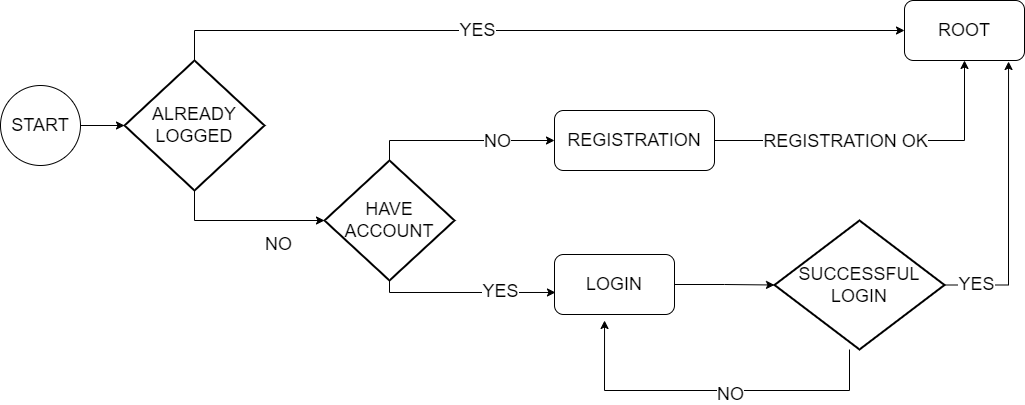
\includegraphics[width=0.8\textwidth, clip]{../../assets/loginFlow.png}
    \end{center}
    \caption{Login flow diagram.}
    \label{fig:loginflow}
\end{figure}

\begin{figure}[h!]
    \begin{center}
        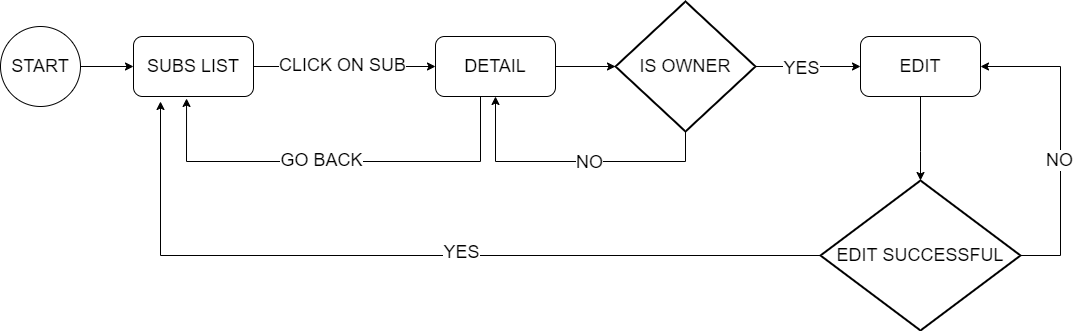
\includegraphics[width=\textwidth, clip]{../../assets/editflow.png}
    \end{center}
    \caption{Login flow diagram.}
    \label{fig:editflow}
\end{figure}


\subsection{Screenshots}
The application design has been enhanced by \textbf{customizing} the interface specifically for smartphone and for tablet. The two devices typical characteristics have been considered during the design phase and this allowed a better implementation, acknowledging pros and cons of the portrait and landscape modes.

In particular, for what concerns the tablet implementation, the \textbf{components sizes} are enhanced, the \textbf{font sizes} are increased as well as the \textbf{layout} is changed in order to allow the maximum number of components to be shown at all times. This is why the main pages show a two-column layout, instead of a single column (portrait mode and smartphone design). A part from this, the design remains consistent, in order not to puzzle the user when changing from one device to another.

\subsubsection{Smartphone Application}

\begin{figure}[h!]
    \centering
    \begin{minipage}[c]{0.45\textwidth}
        \centering
        \includegraphics[width=0.6\textwidth, clip]{../../assets/smartphone/login.PNG}
        \caption{Login page}
        \label{fig:login}
    \end{minipage}\hspace{1cm}%
    \begin{minipage}[c]{0.45\textwidth}
        \centering
        \includegraphics[width=0.6\textwidth, clip]{../../assets/smartphone/reg.PNG}
        \caption{Registration page}
        \label{fig:reg}
    \end{minipage}
\end{figure}

\begin{figure}[h!]
    \centering
    \begin{minipage}[c]{0.45\textwidth}
        \centering
        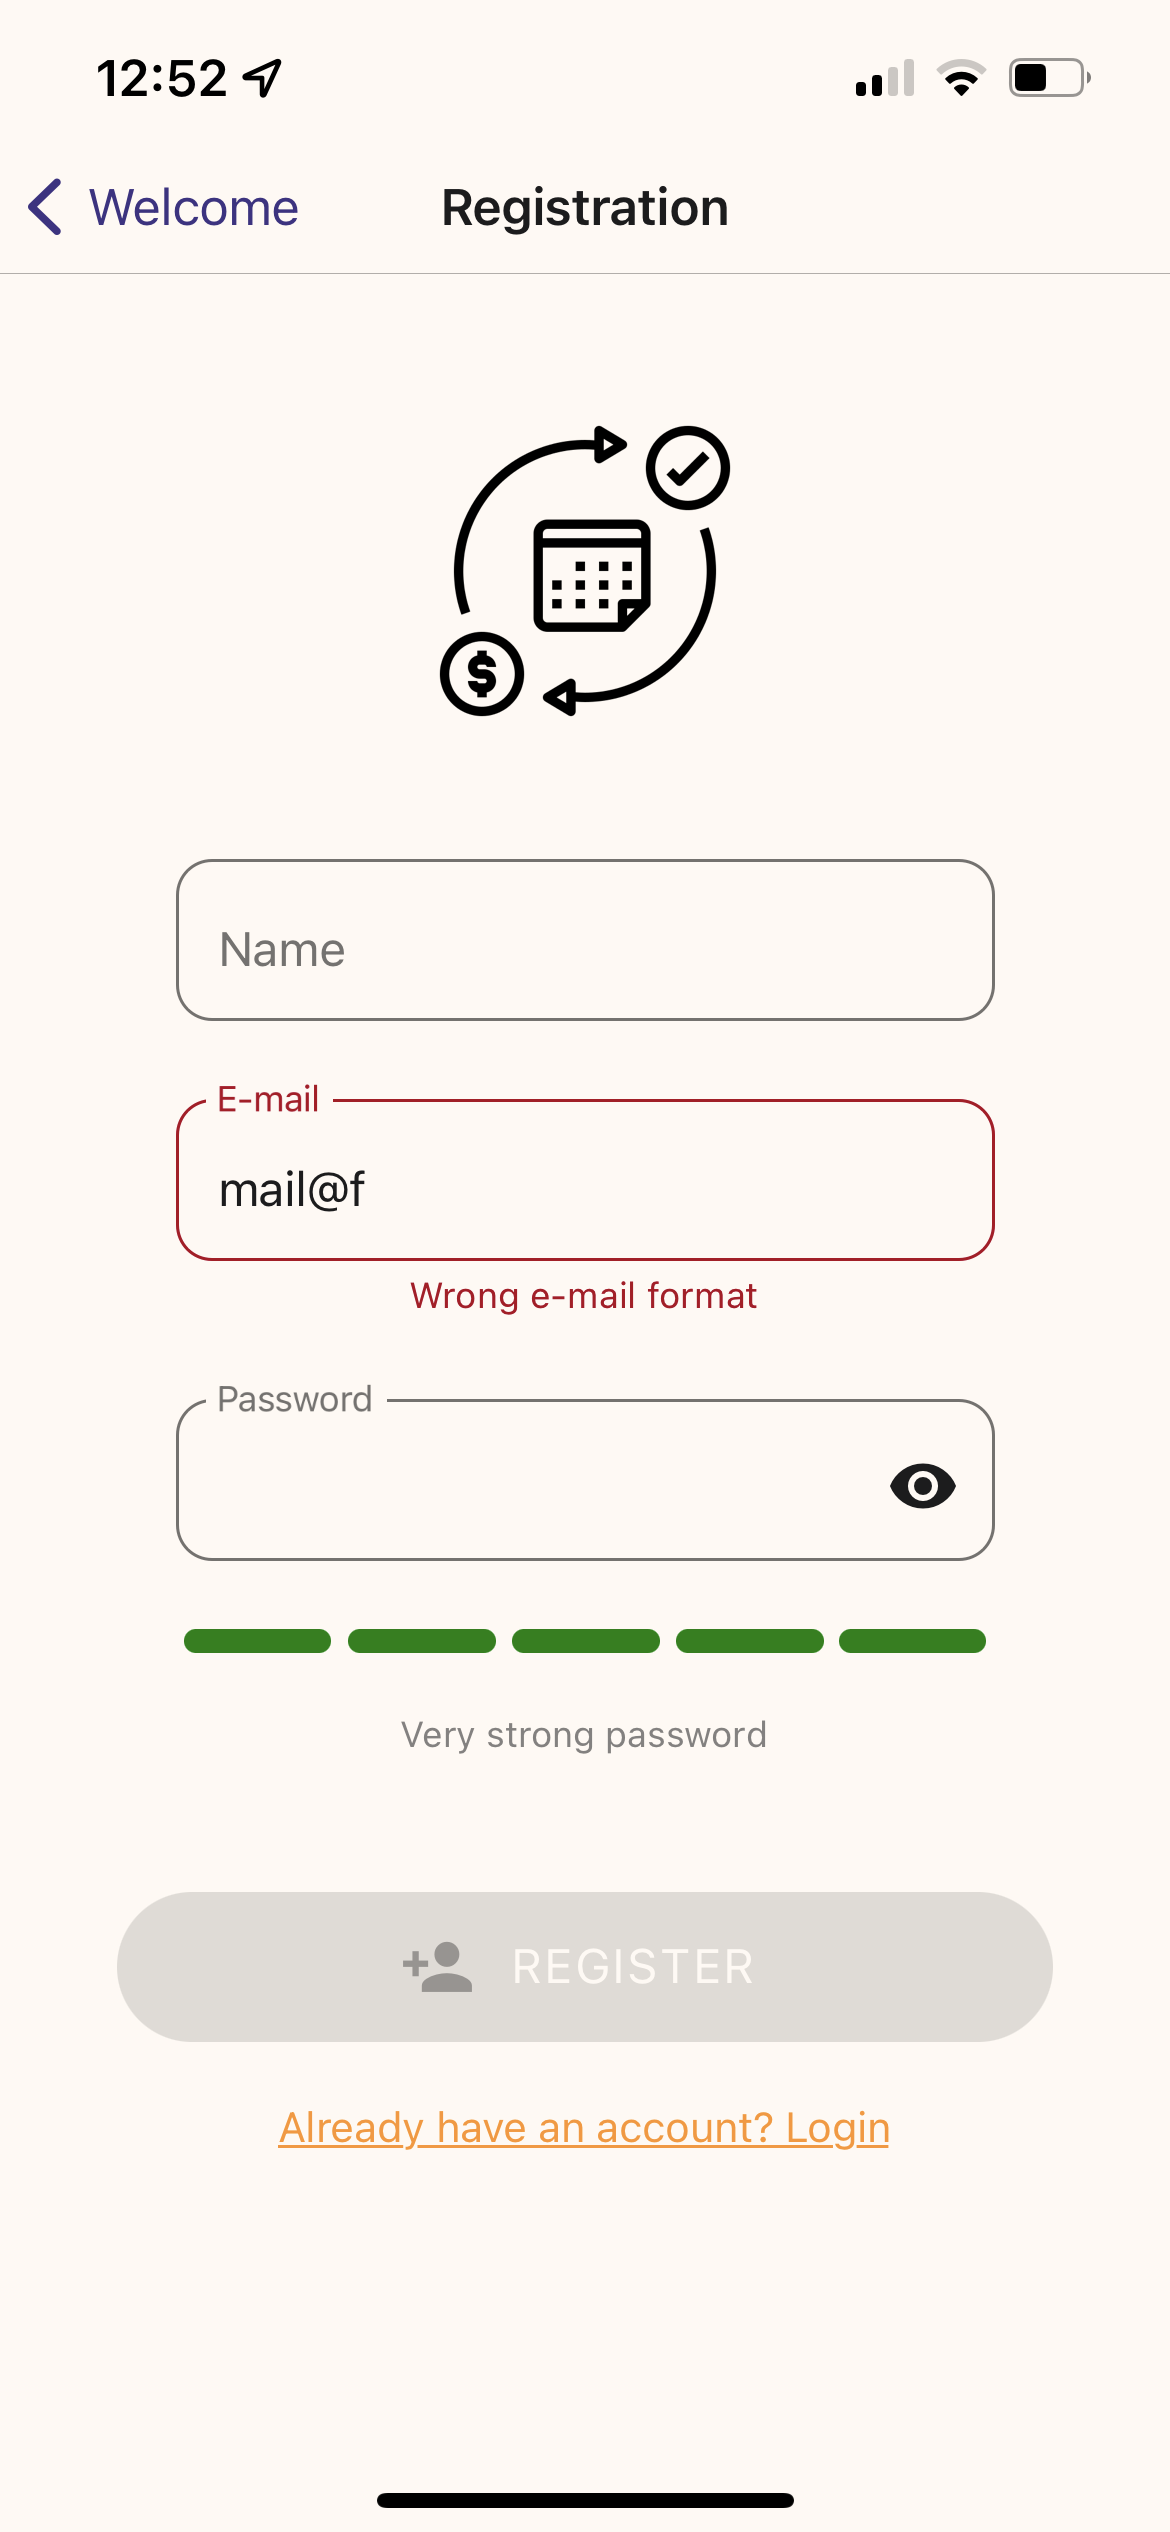
\includegraphics[width=0.6\textwidth, clip]{../../assets/smartphone/regFill.PNG}
        \caption{Input checks for e-mail format and password}
        \label{fig:rfill}
    \end{minipage}\hspace{1cm}%
    \begin{minipage}[c]{0.45\textwidth}
        \centering
        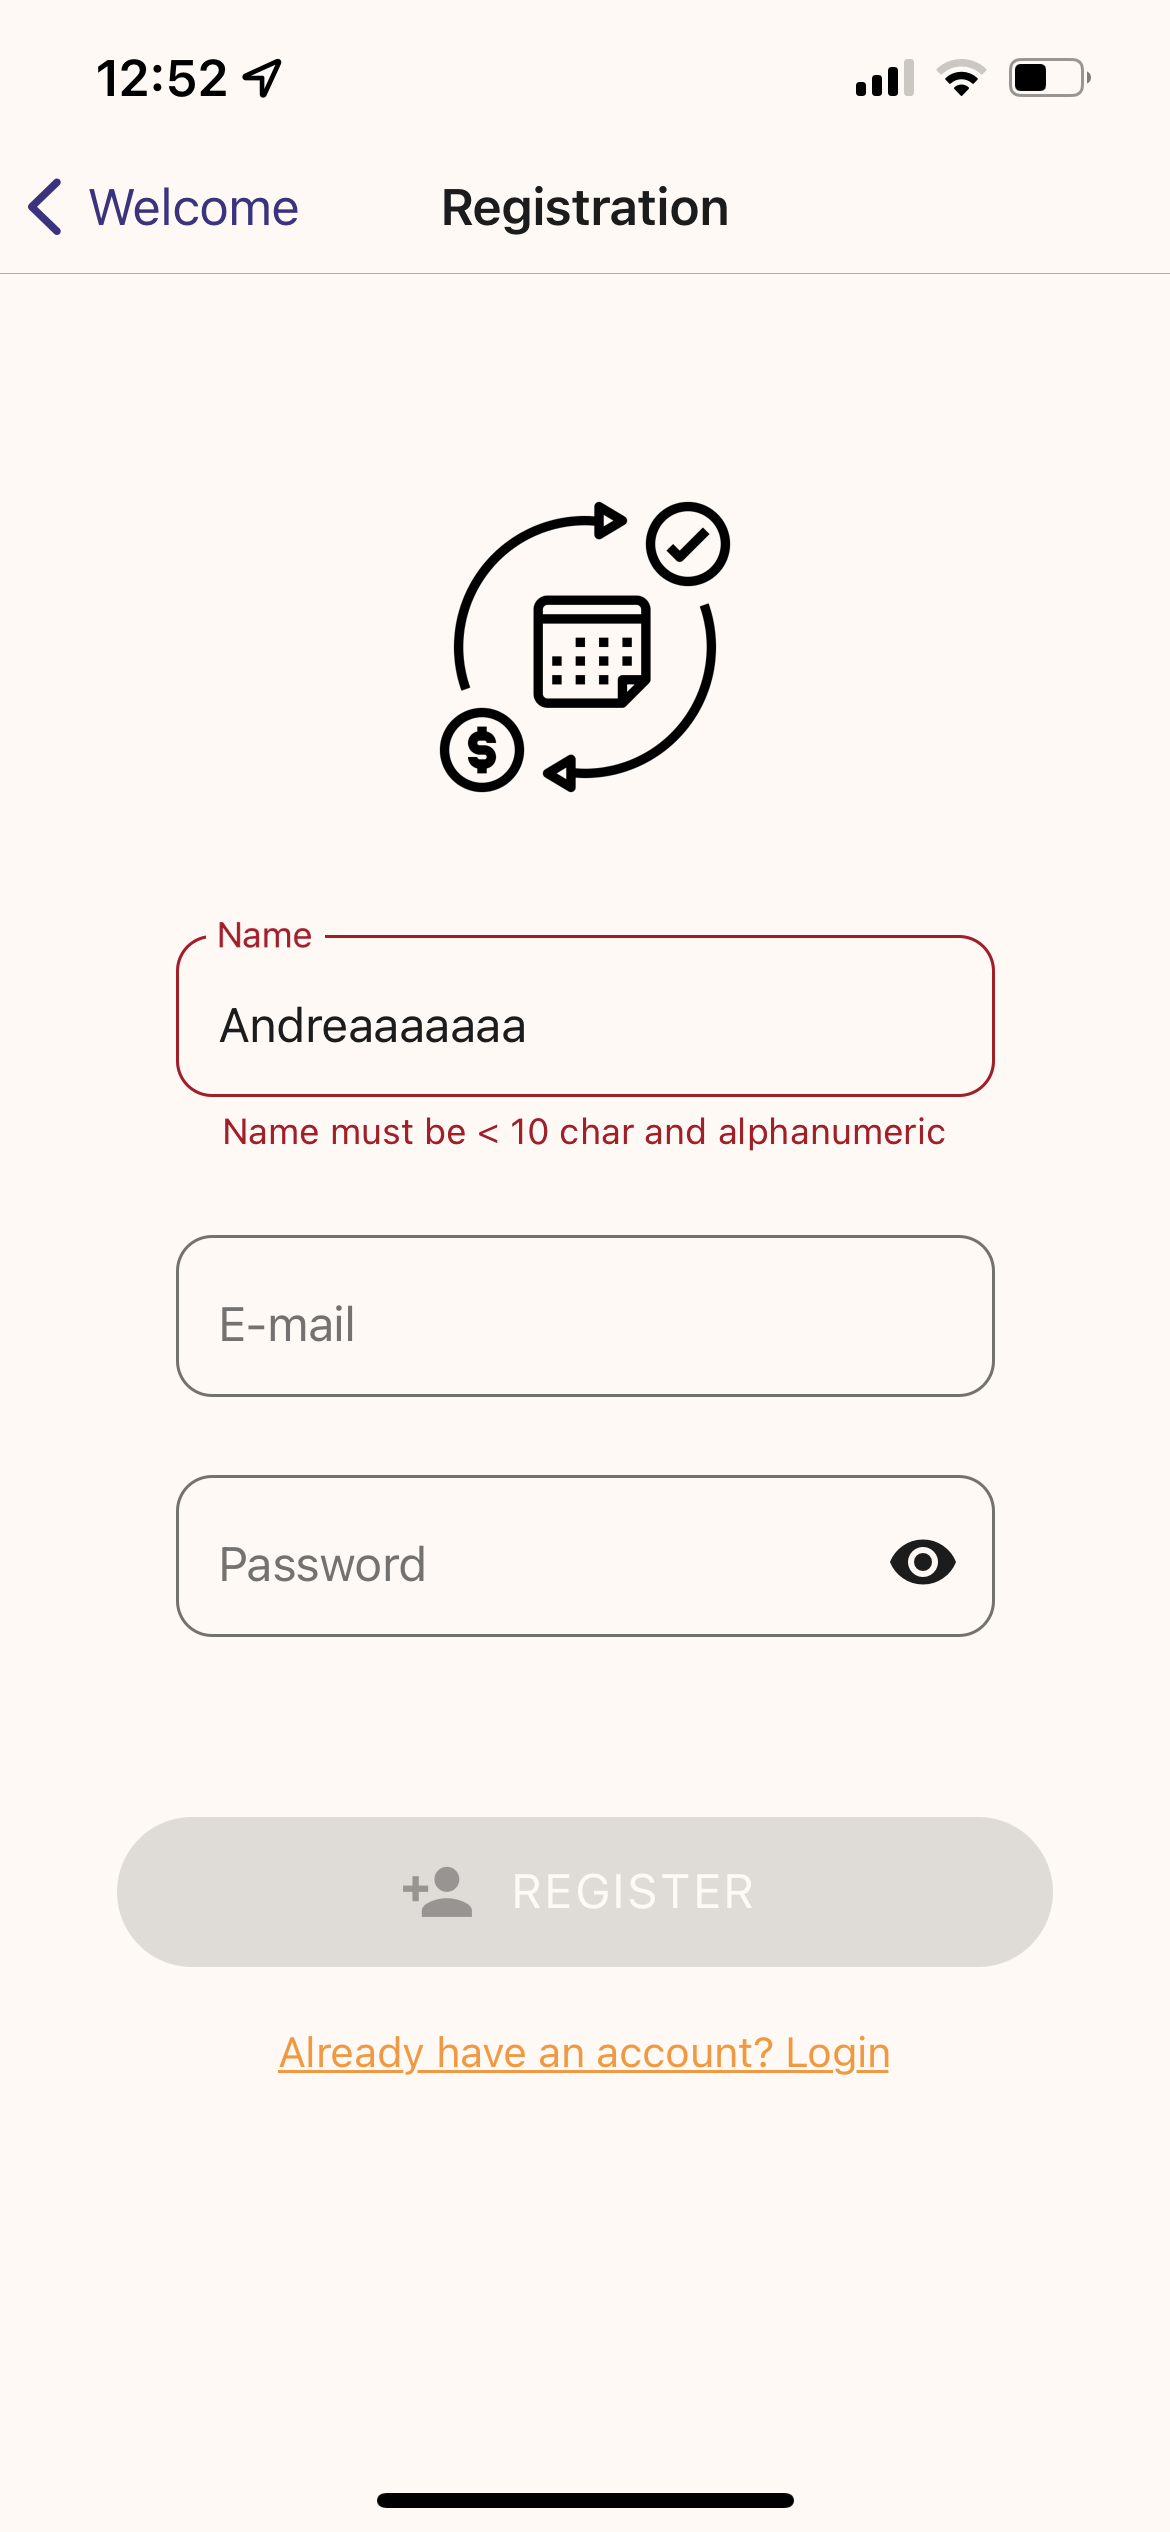
\includegraphics[width=0.6\textwidth, clip]{../../assets/smartphone/regName.PNG}
        \caption{Input checks for the name}
        \label{fig:rname}
    \end{minipage}
\end{figure}

\begin{figure}[h!]
    \centering
    \begin{minipage}[c]{0.45\textwidth}
        \centering
        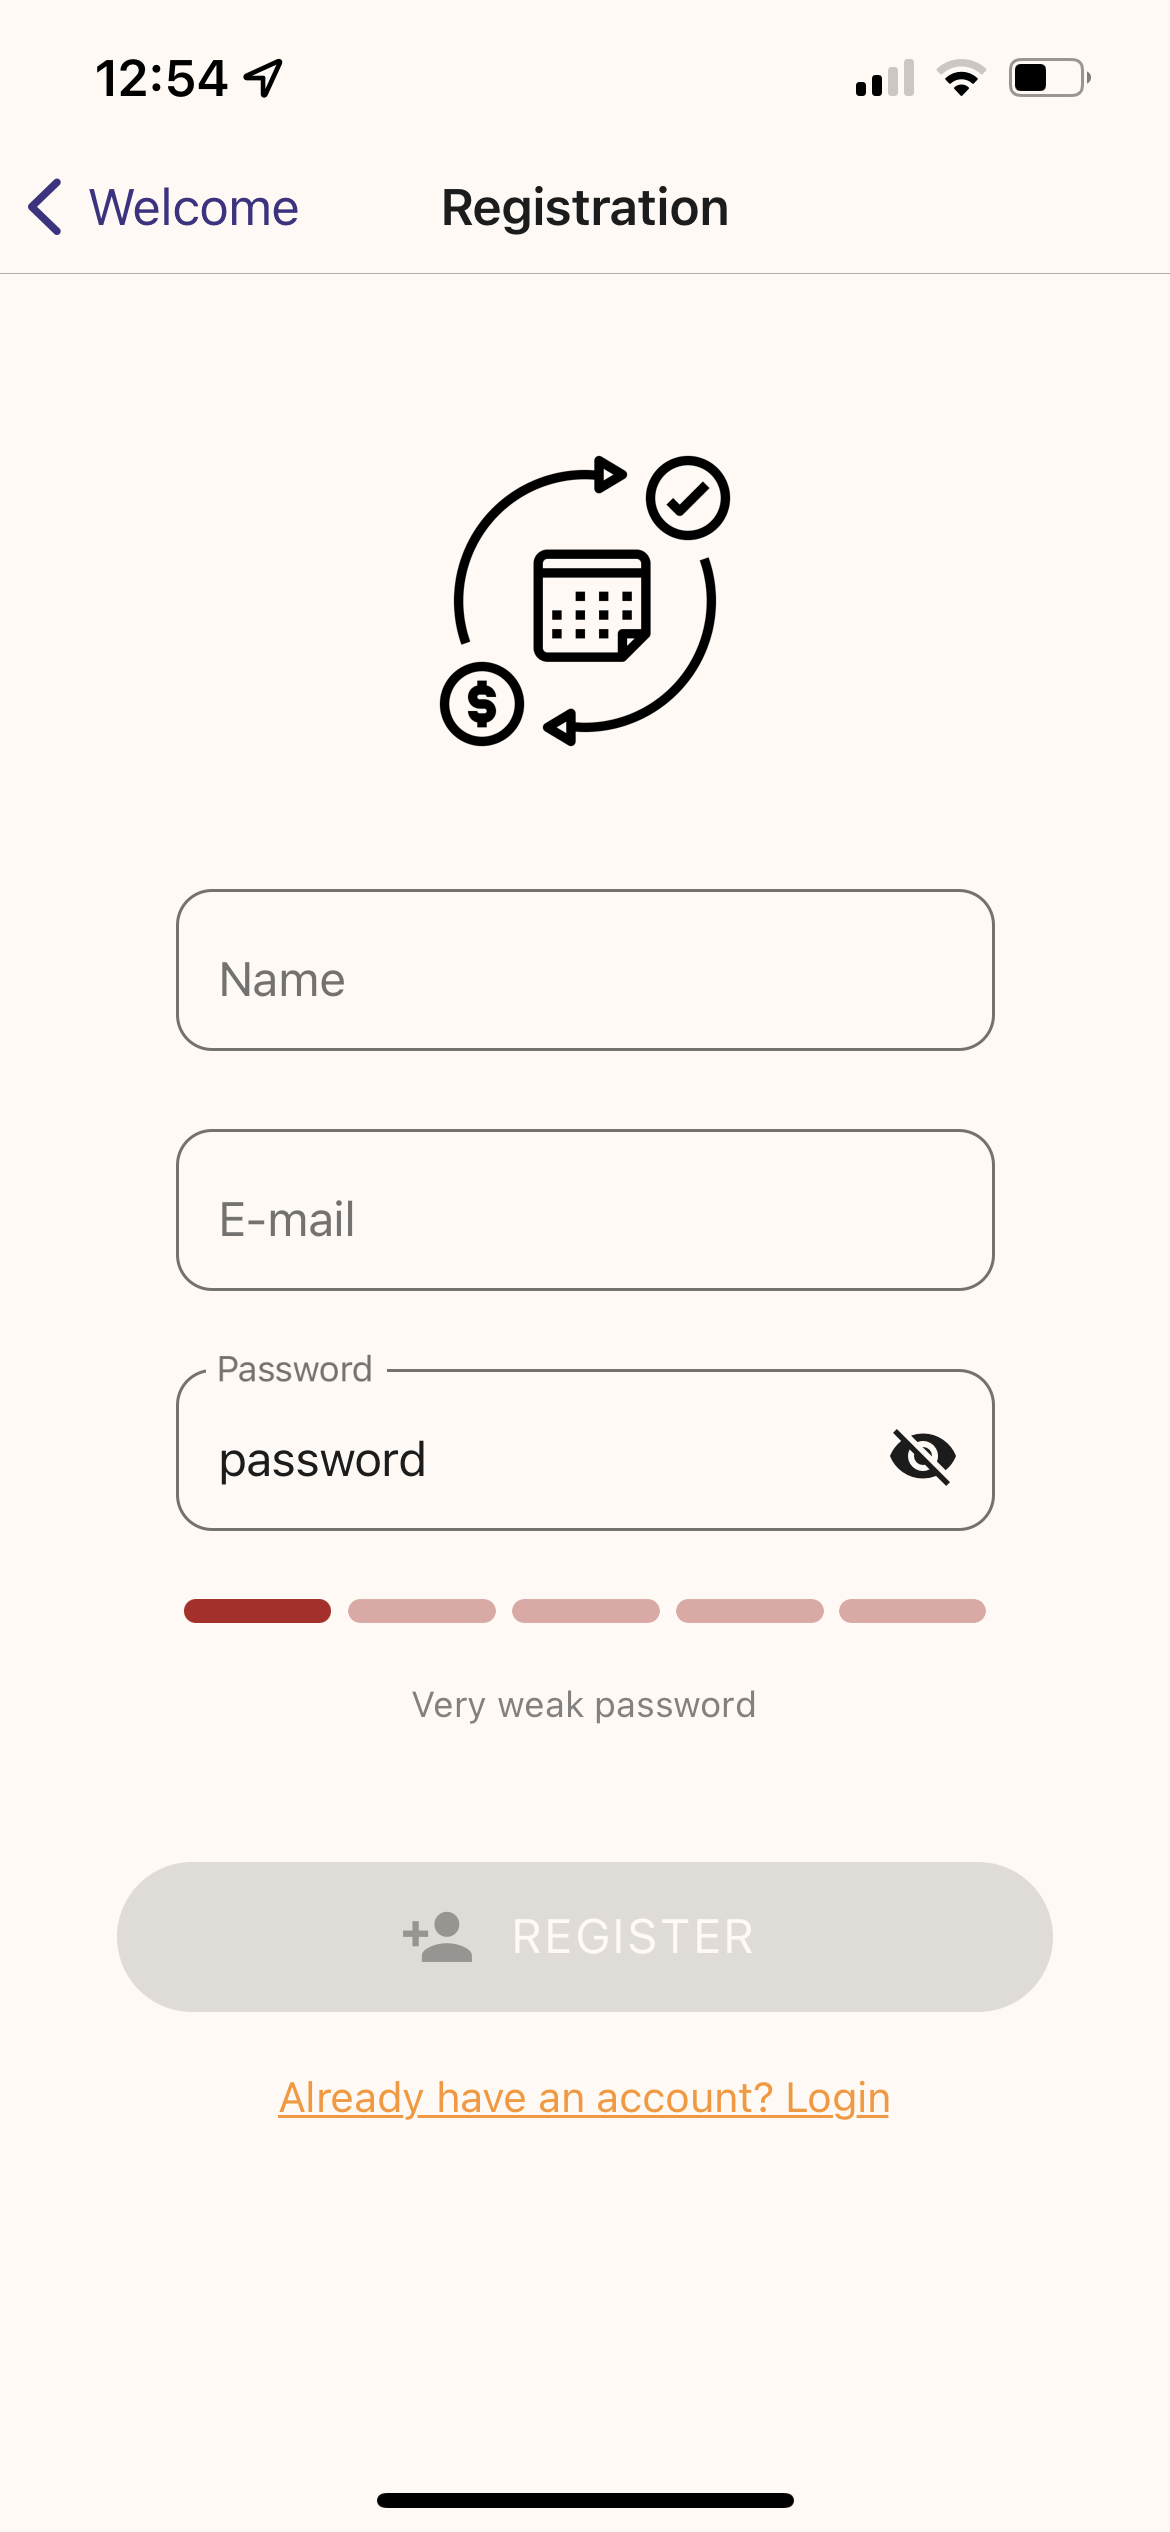
\includegraphics[width=0.6\textwidth, clip]{../../assets/smartphone/weak.PNG}
        \caption{Weak password sign}
        \label{fig:weak}
    \end{minipage}\hspace{1cm}%
    \begin{minipage}[c]{0.45\textwidth}
        \centering
        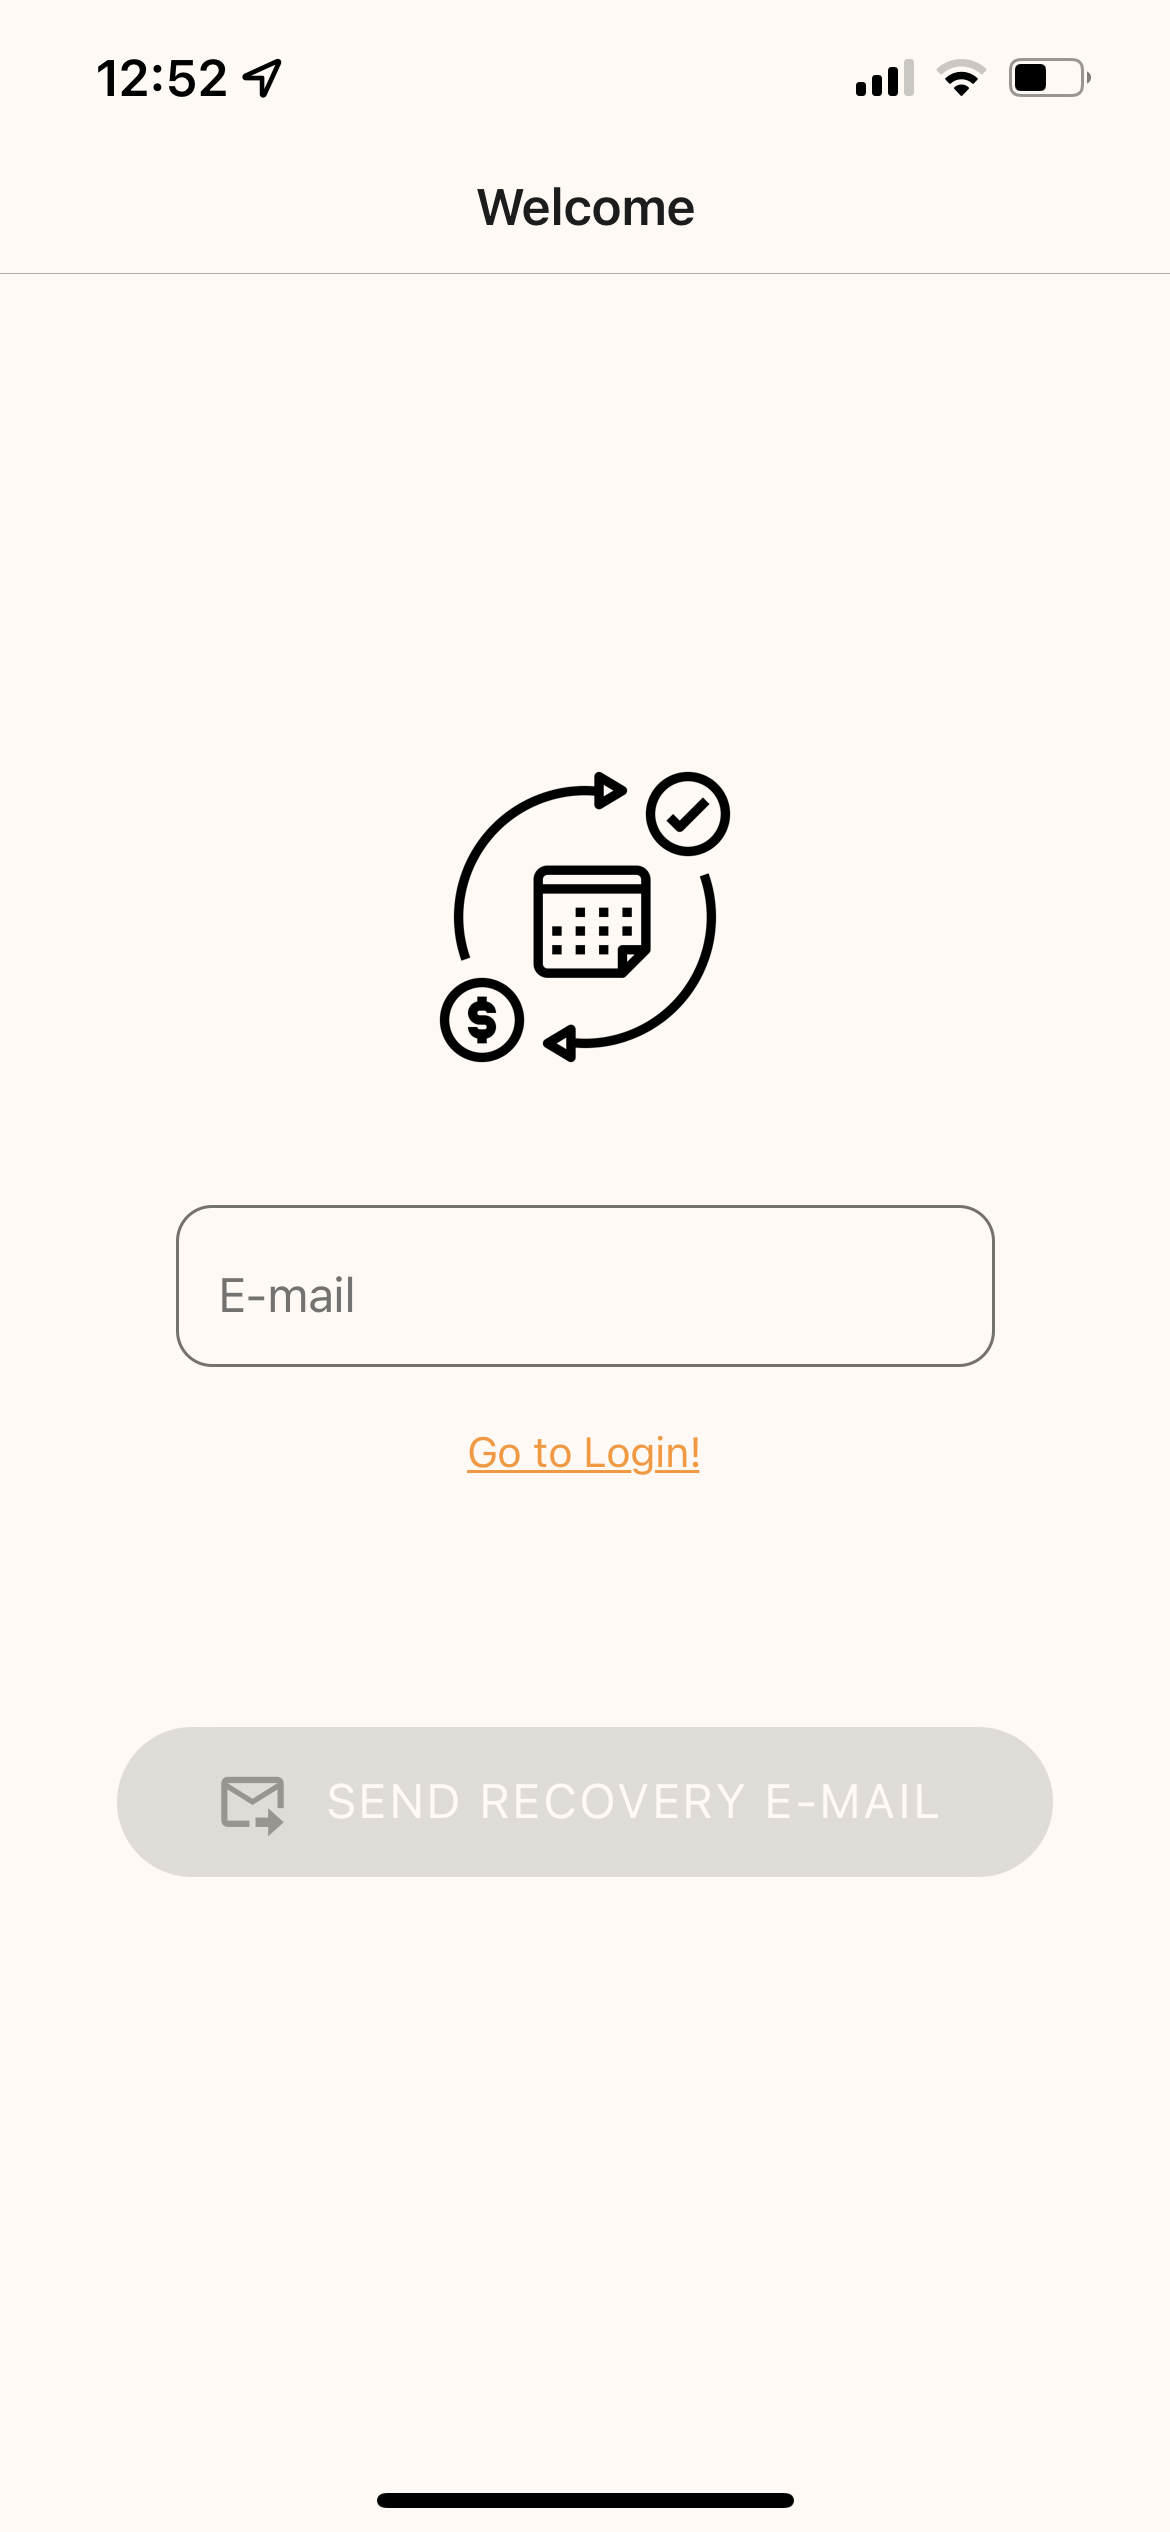
\includegraphics[width=0.6\textwidth, clip]{../../assets/smartphone/forgot.PNG}
        \caption{Password reset page}
        \label{fig:forgot}
    \end{minipage}
\end{figure}

\begin{figure}[h!]
    \centering
    \begin{minipage}[c]{0.45\textwidth}
        \centering
        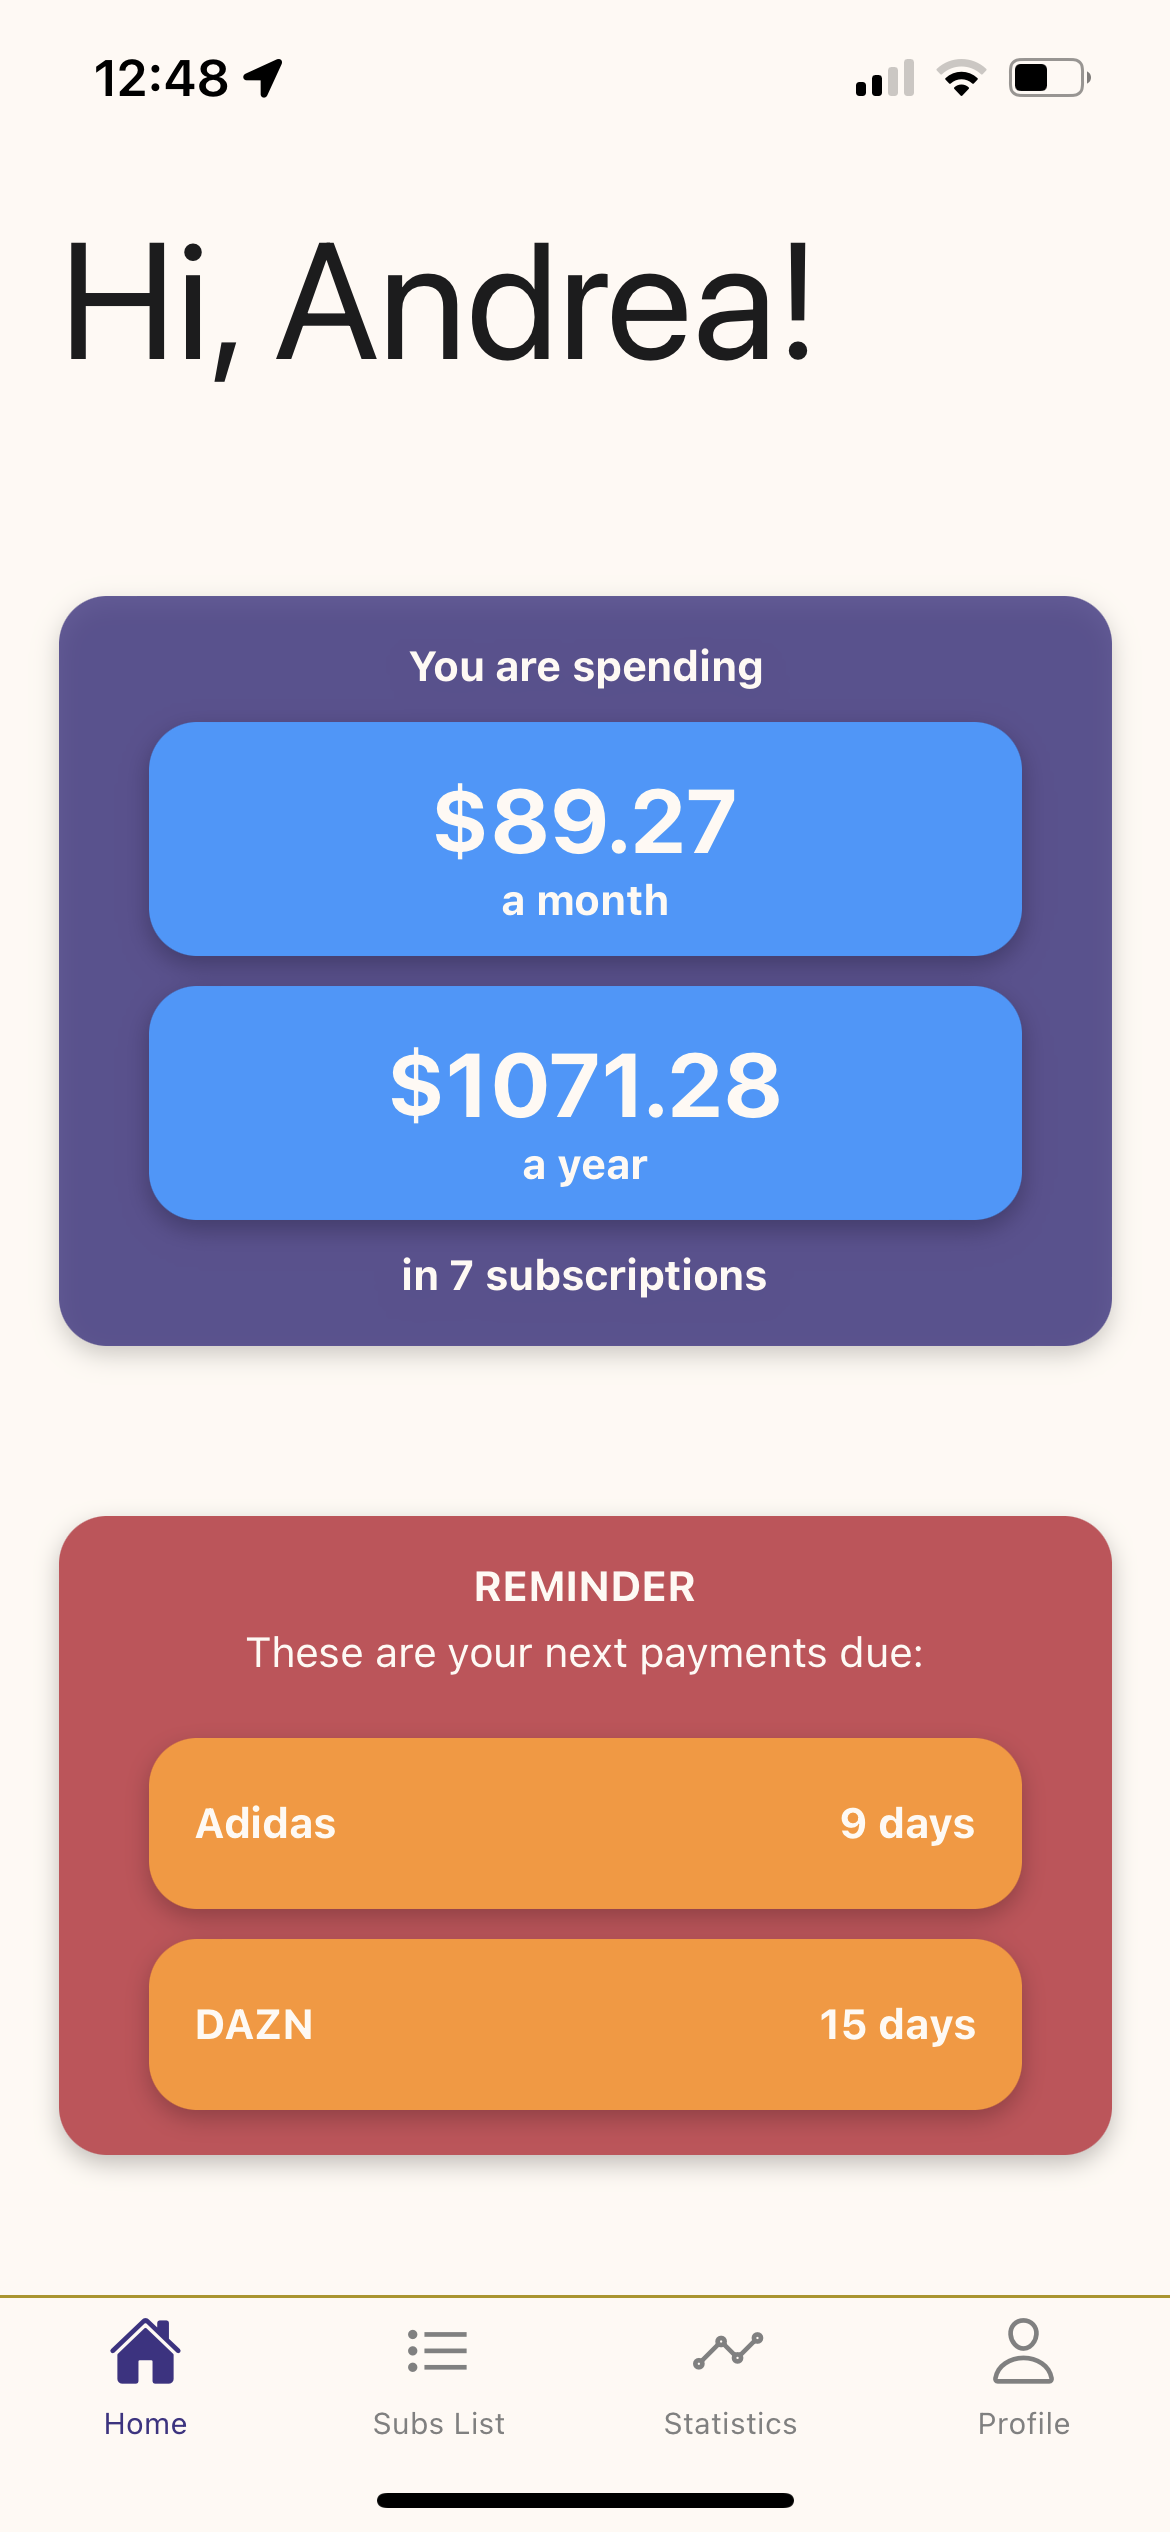
\includegraphics[width=0.6\textwidth, clip]{../../assets/smartphone/home.PNG}
        \caption{Home screen}
        \label{fig:home}
    \end{minipage}\hspace{1cm}%
    \begin{minipage}[c]{0.45\textwidth}
        \centering
        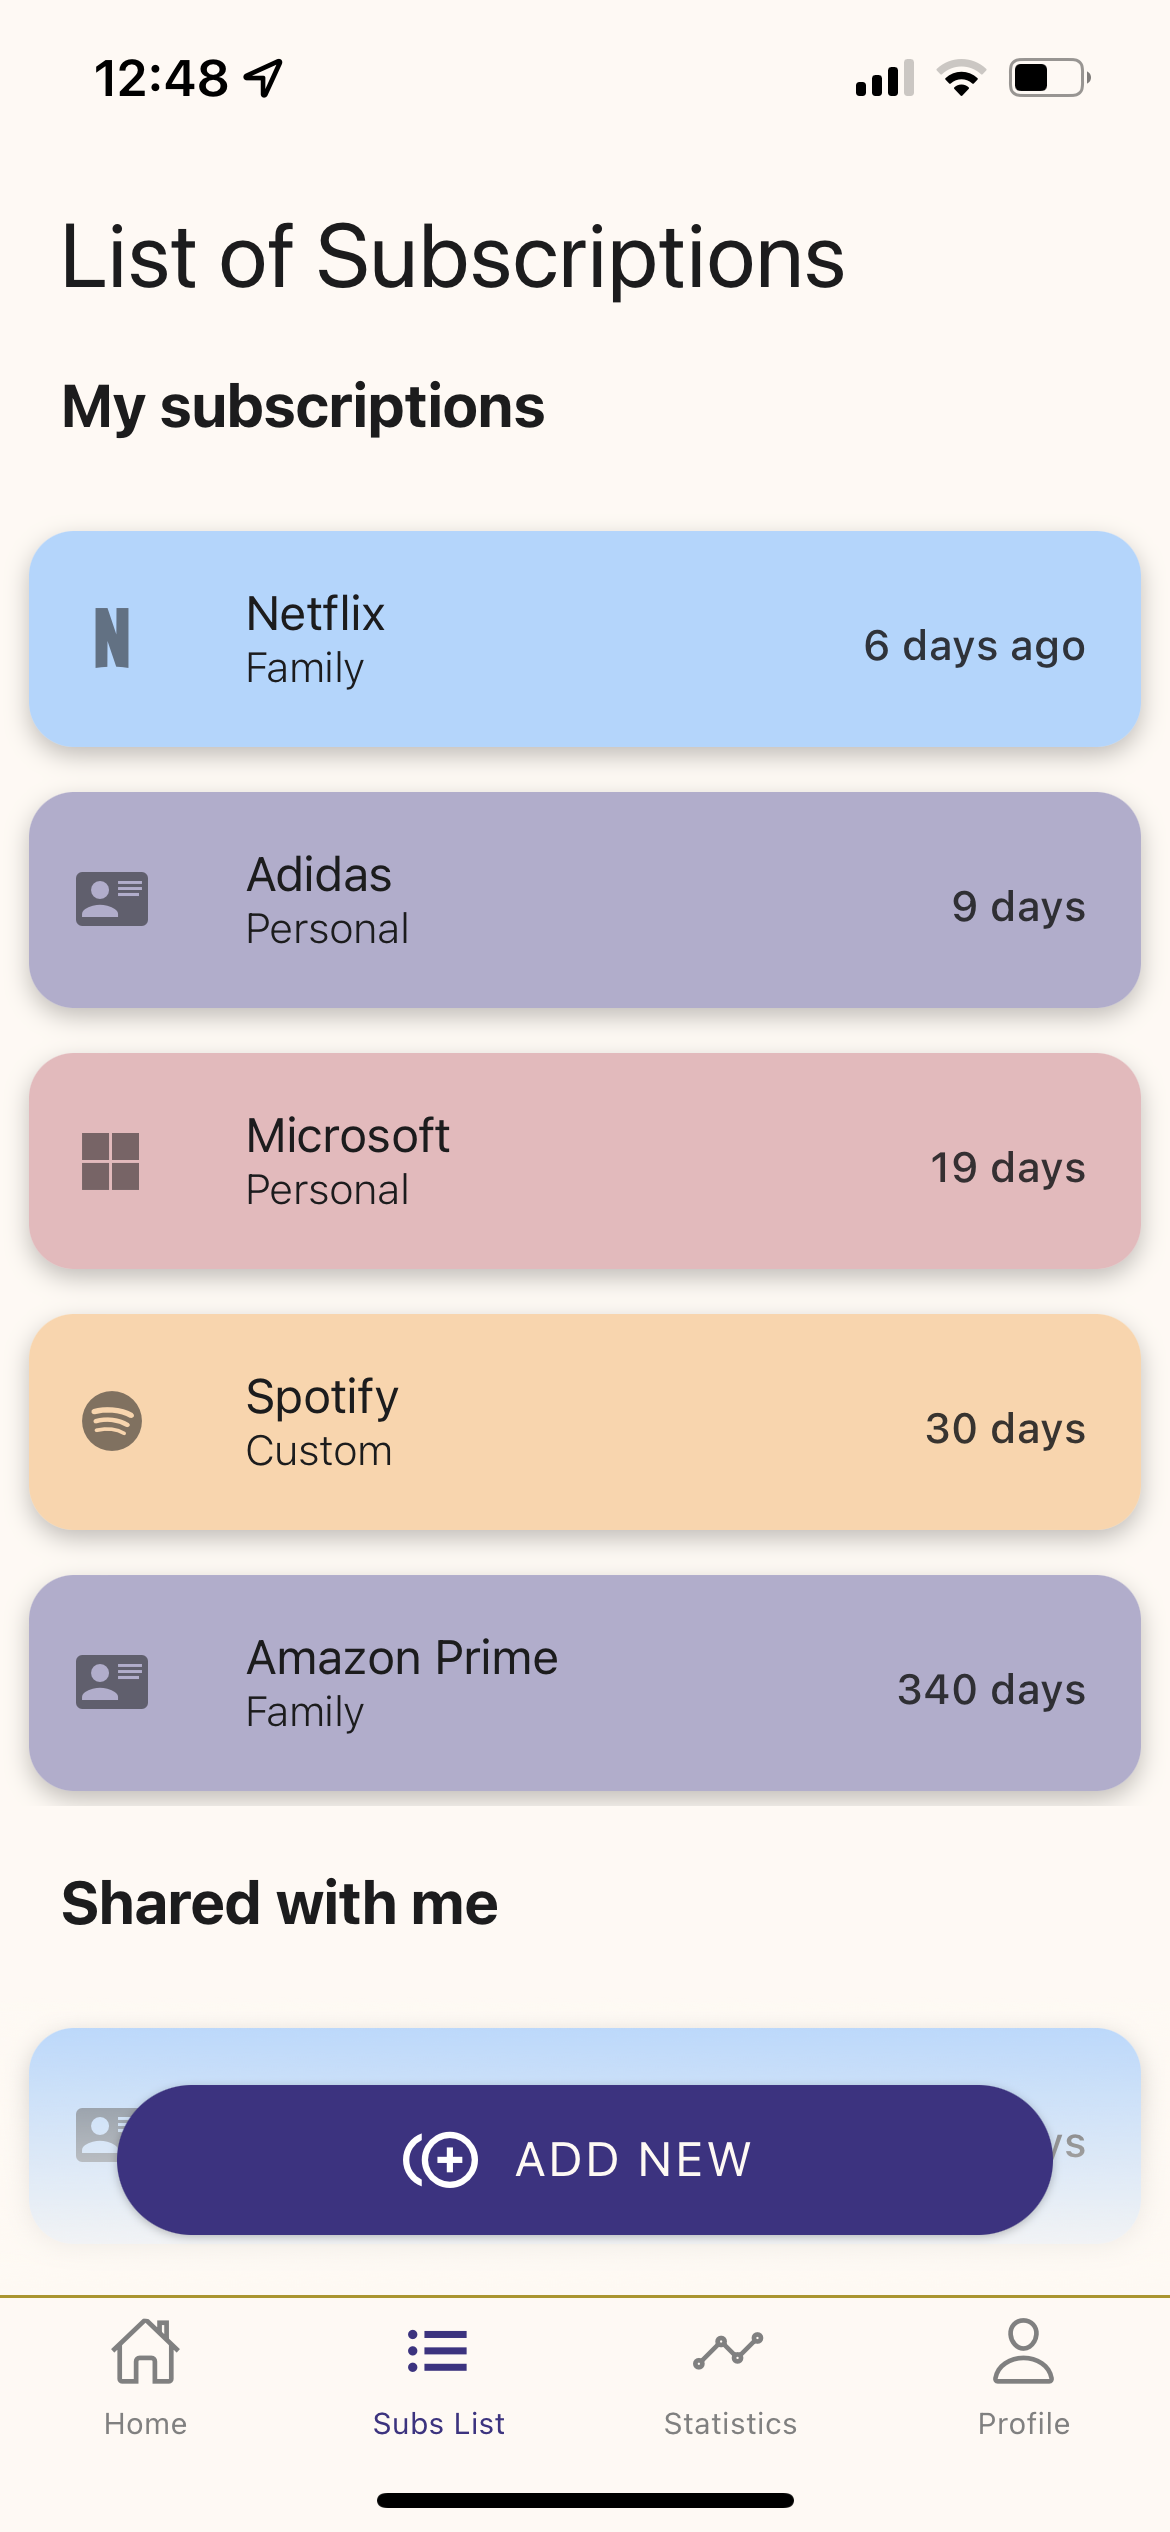
\includegraphics[width=0.6\textwidth, clip]{../../assets/smartphone/subsList.PNG}
        \caption{List of subscriptions}
        \label{fig:subsList}
    \end{minipage}
\end{figure}

\begin{figure}[h!]
    \centering
    \begin{minipage}[c]{0.45\textwidth}
        \centering
        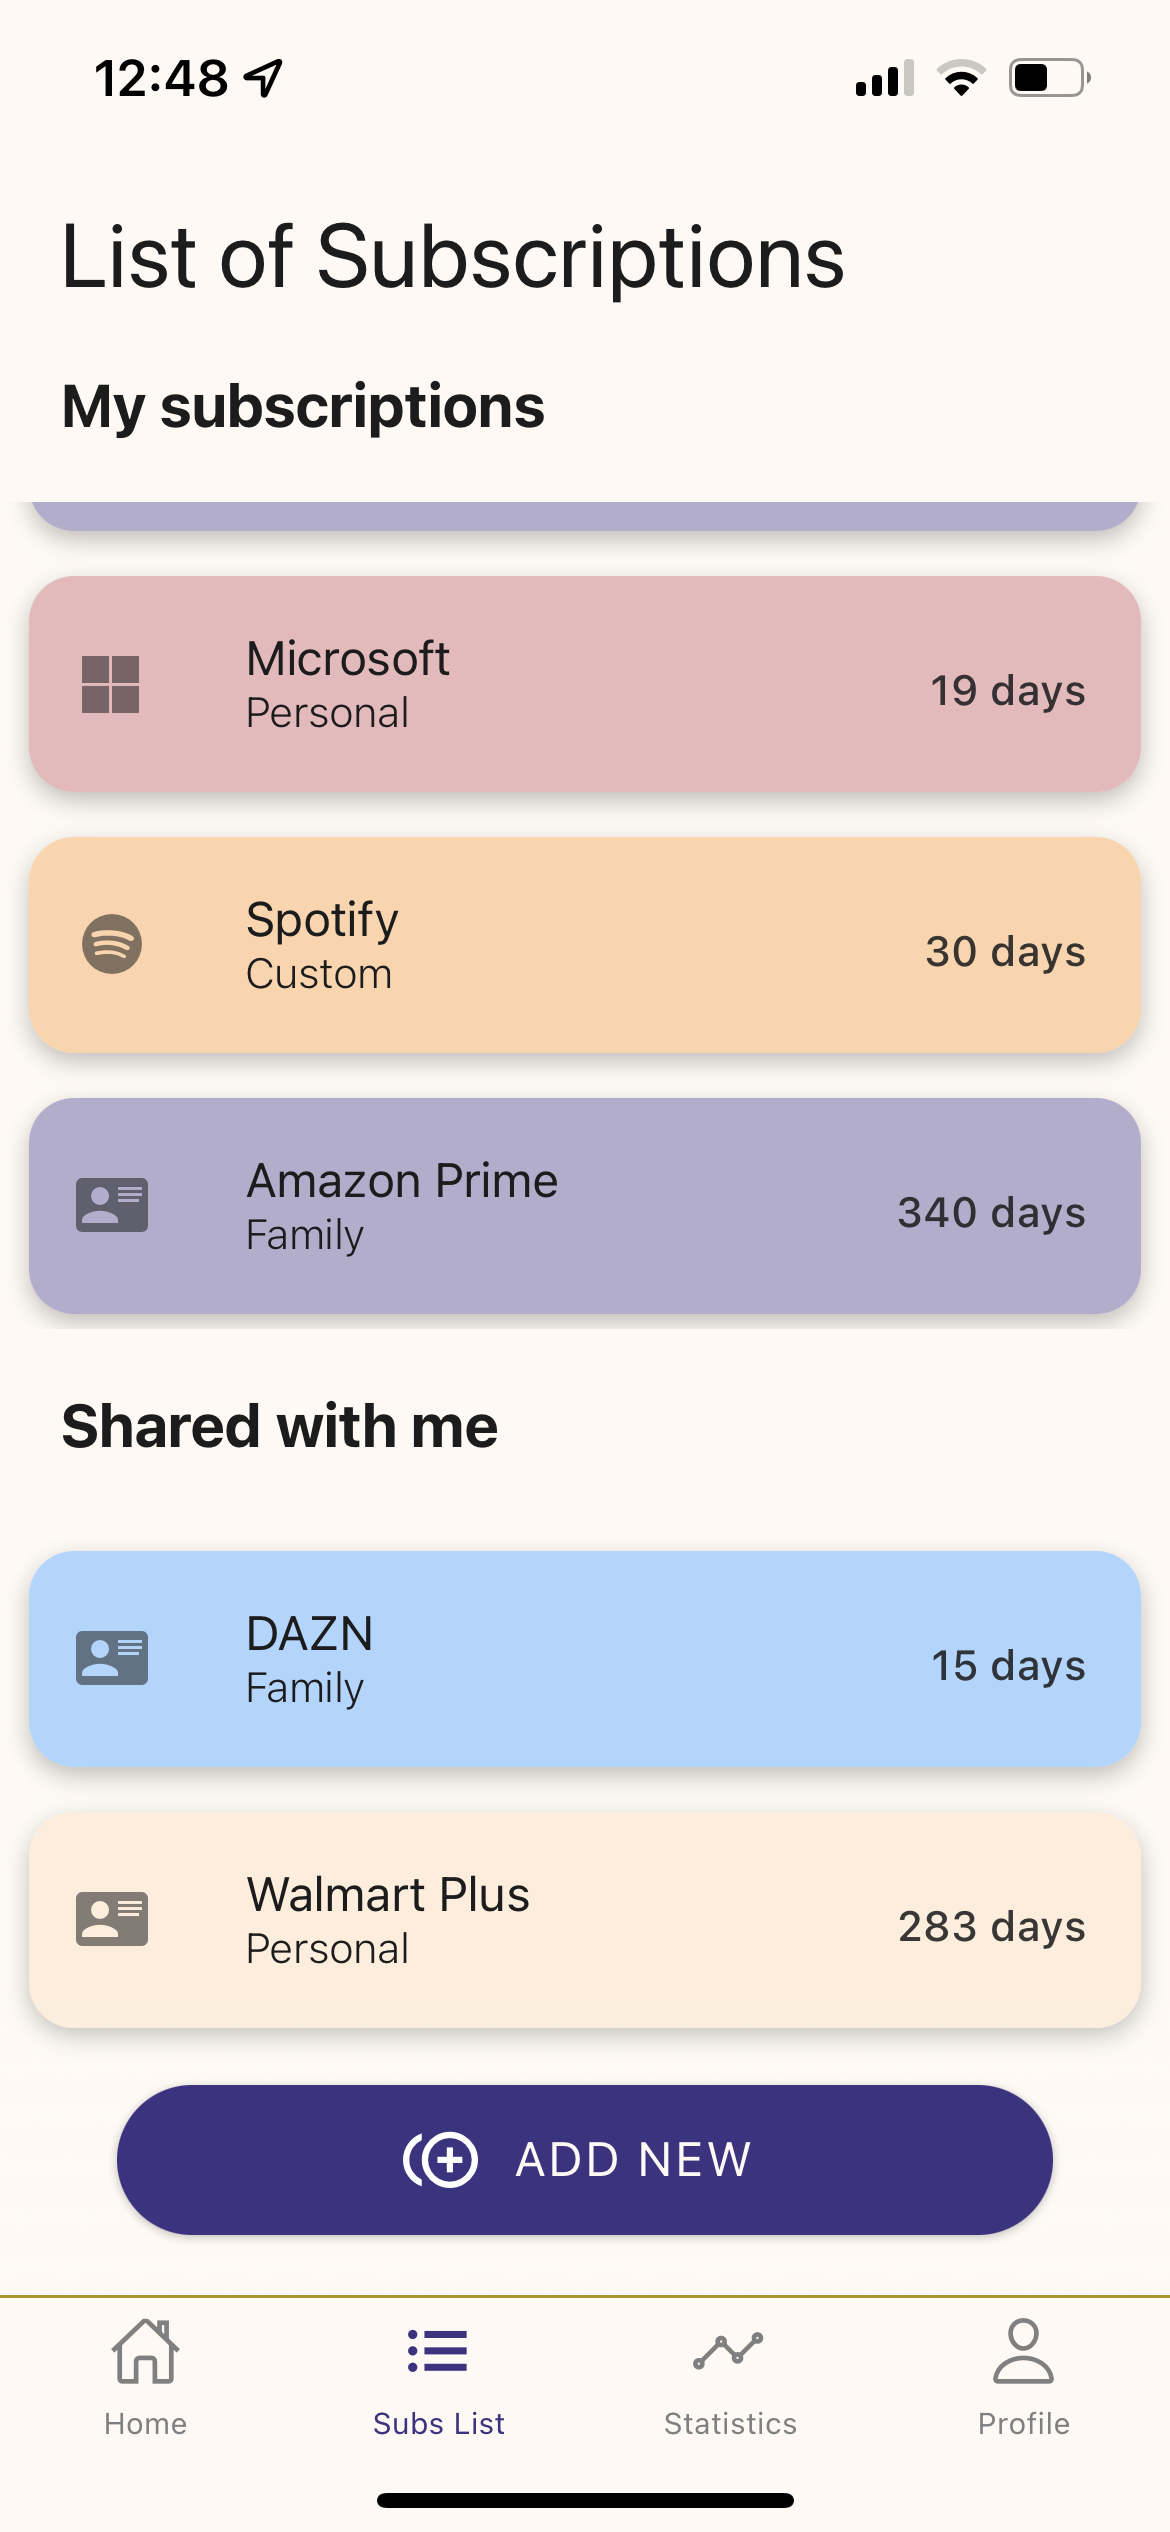
\includegraphics[width=0.6\textwidth, clip]{../../assets/smartphone/subsList2.PNG}
        \caption{Both `my subscriptions' and `shared with me'}
        \label{fig:subsList2}
    \end{minipage}\hspace{1cm}%
    \begin{minipage}[c]{0.45\textwidth}
        \centering
        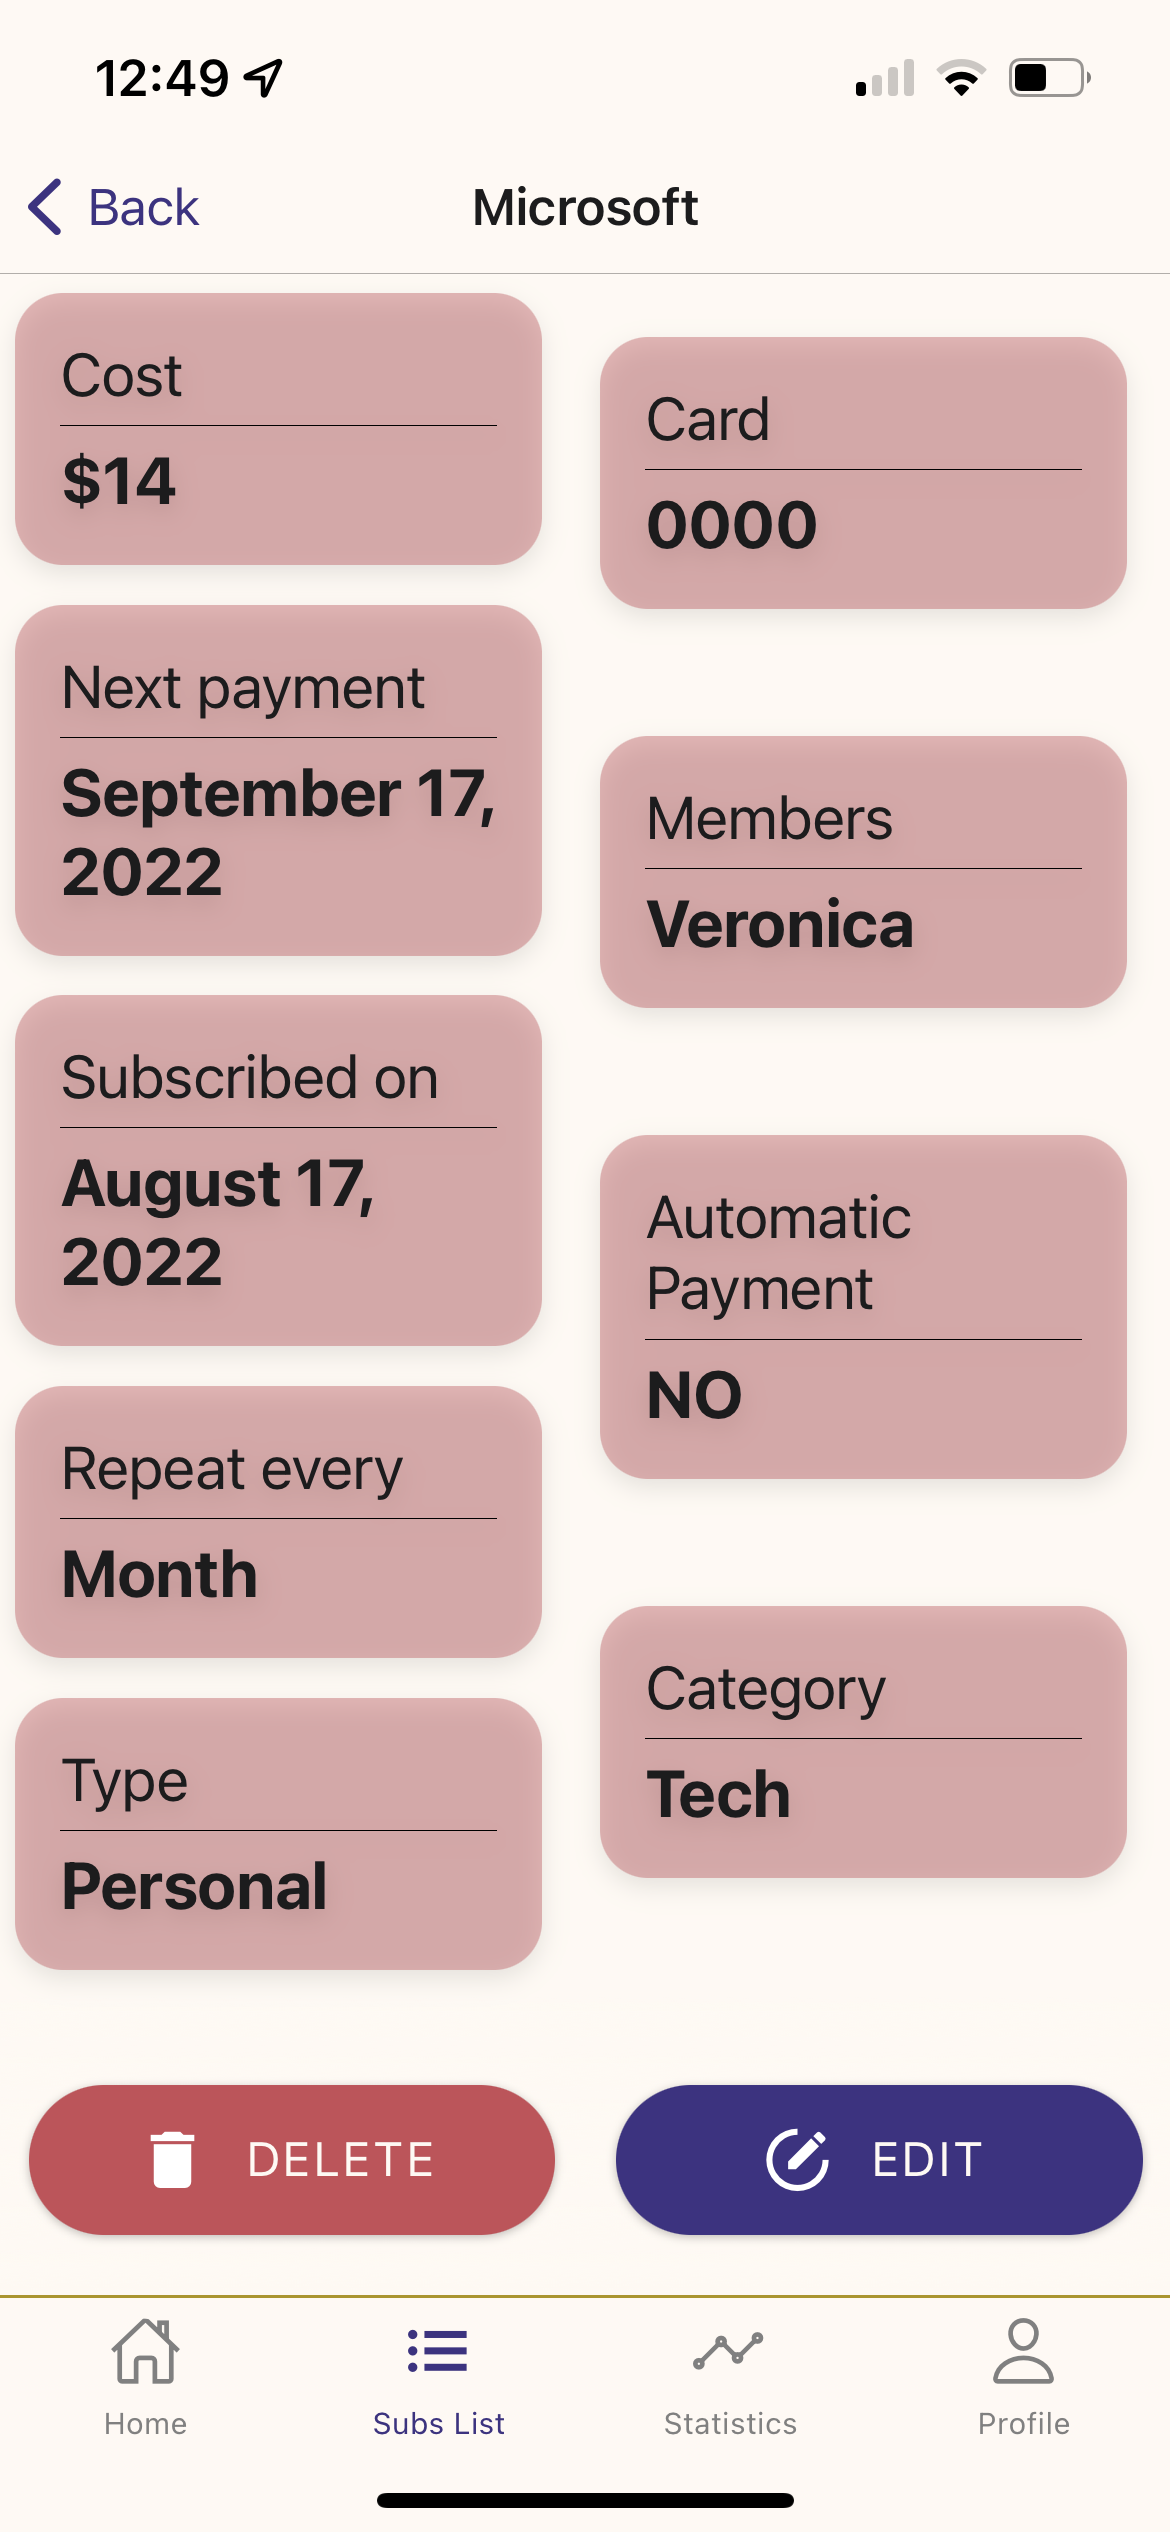
\includegraphics[width=0.6\textwidth, clip]{../../assets/smartphone/detail.PNG}
        \caption{Subscription detail card}
        \label{fig:detail}
    \end{minipage}
\end{figure}

\begin{figure}[h!]
    \centering
    \begin{minipage}[c]{0.45\textwidth}
        \centering
        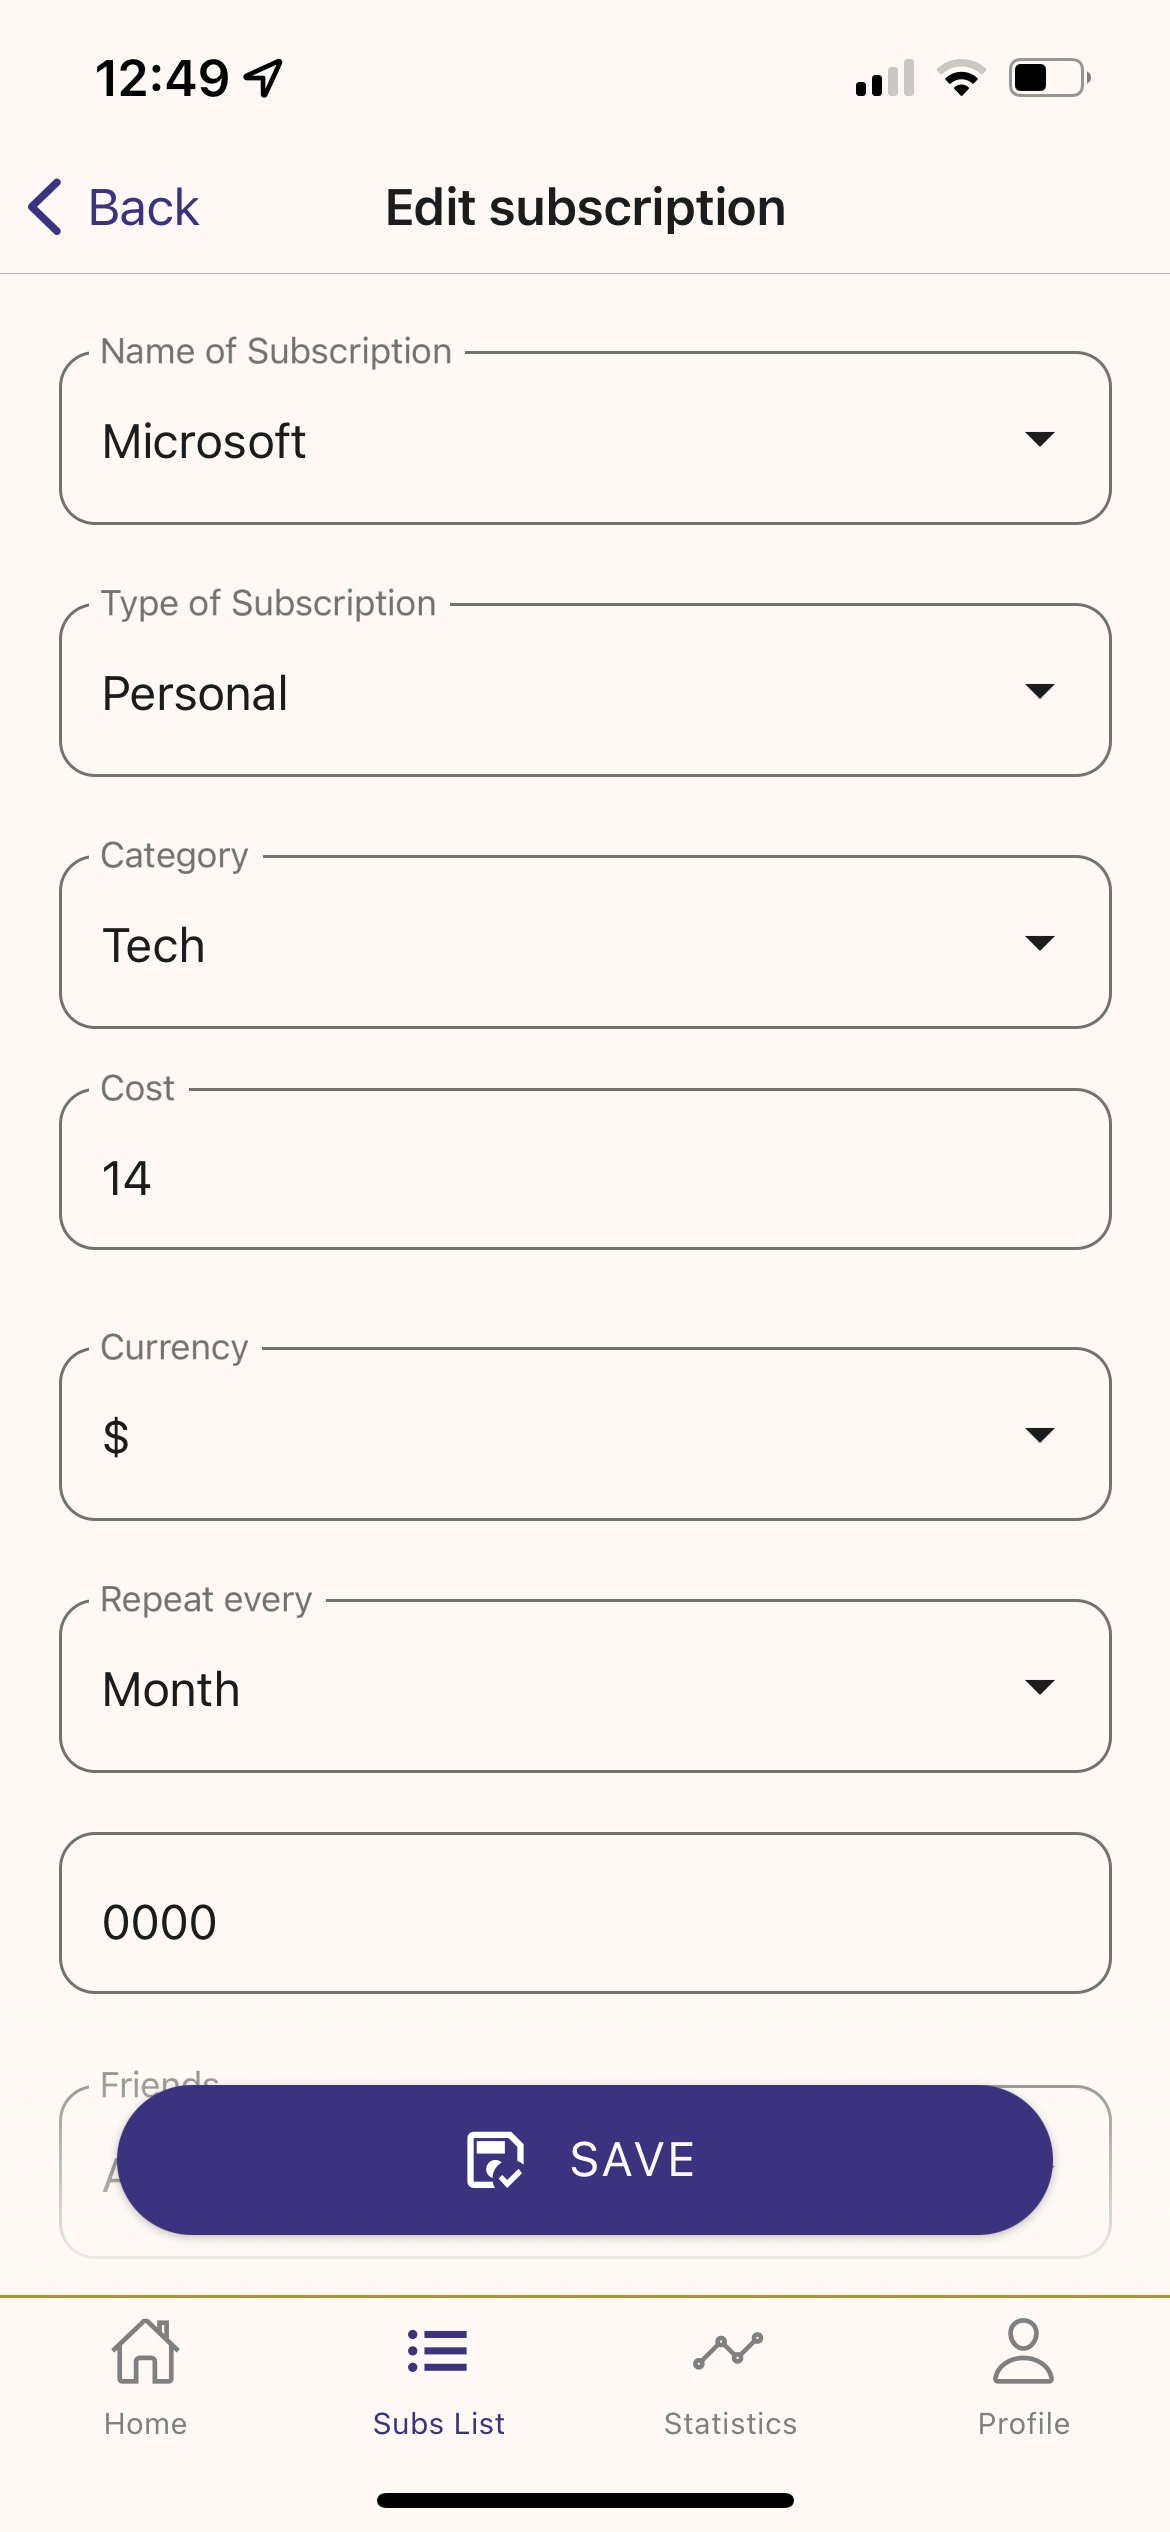
\includegraphics[width=0.6\textwidth, clip]{../../assets/smartphone/edit.PNG}
        \caption{Edit page: already filled form}
        \label{fig:edit}
    \end{minipage}\hspace{1cm}%
    \begin{minipage}[c]{0.45\textwidth}
        \centering
        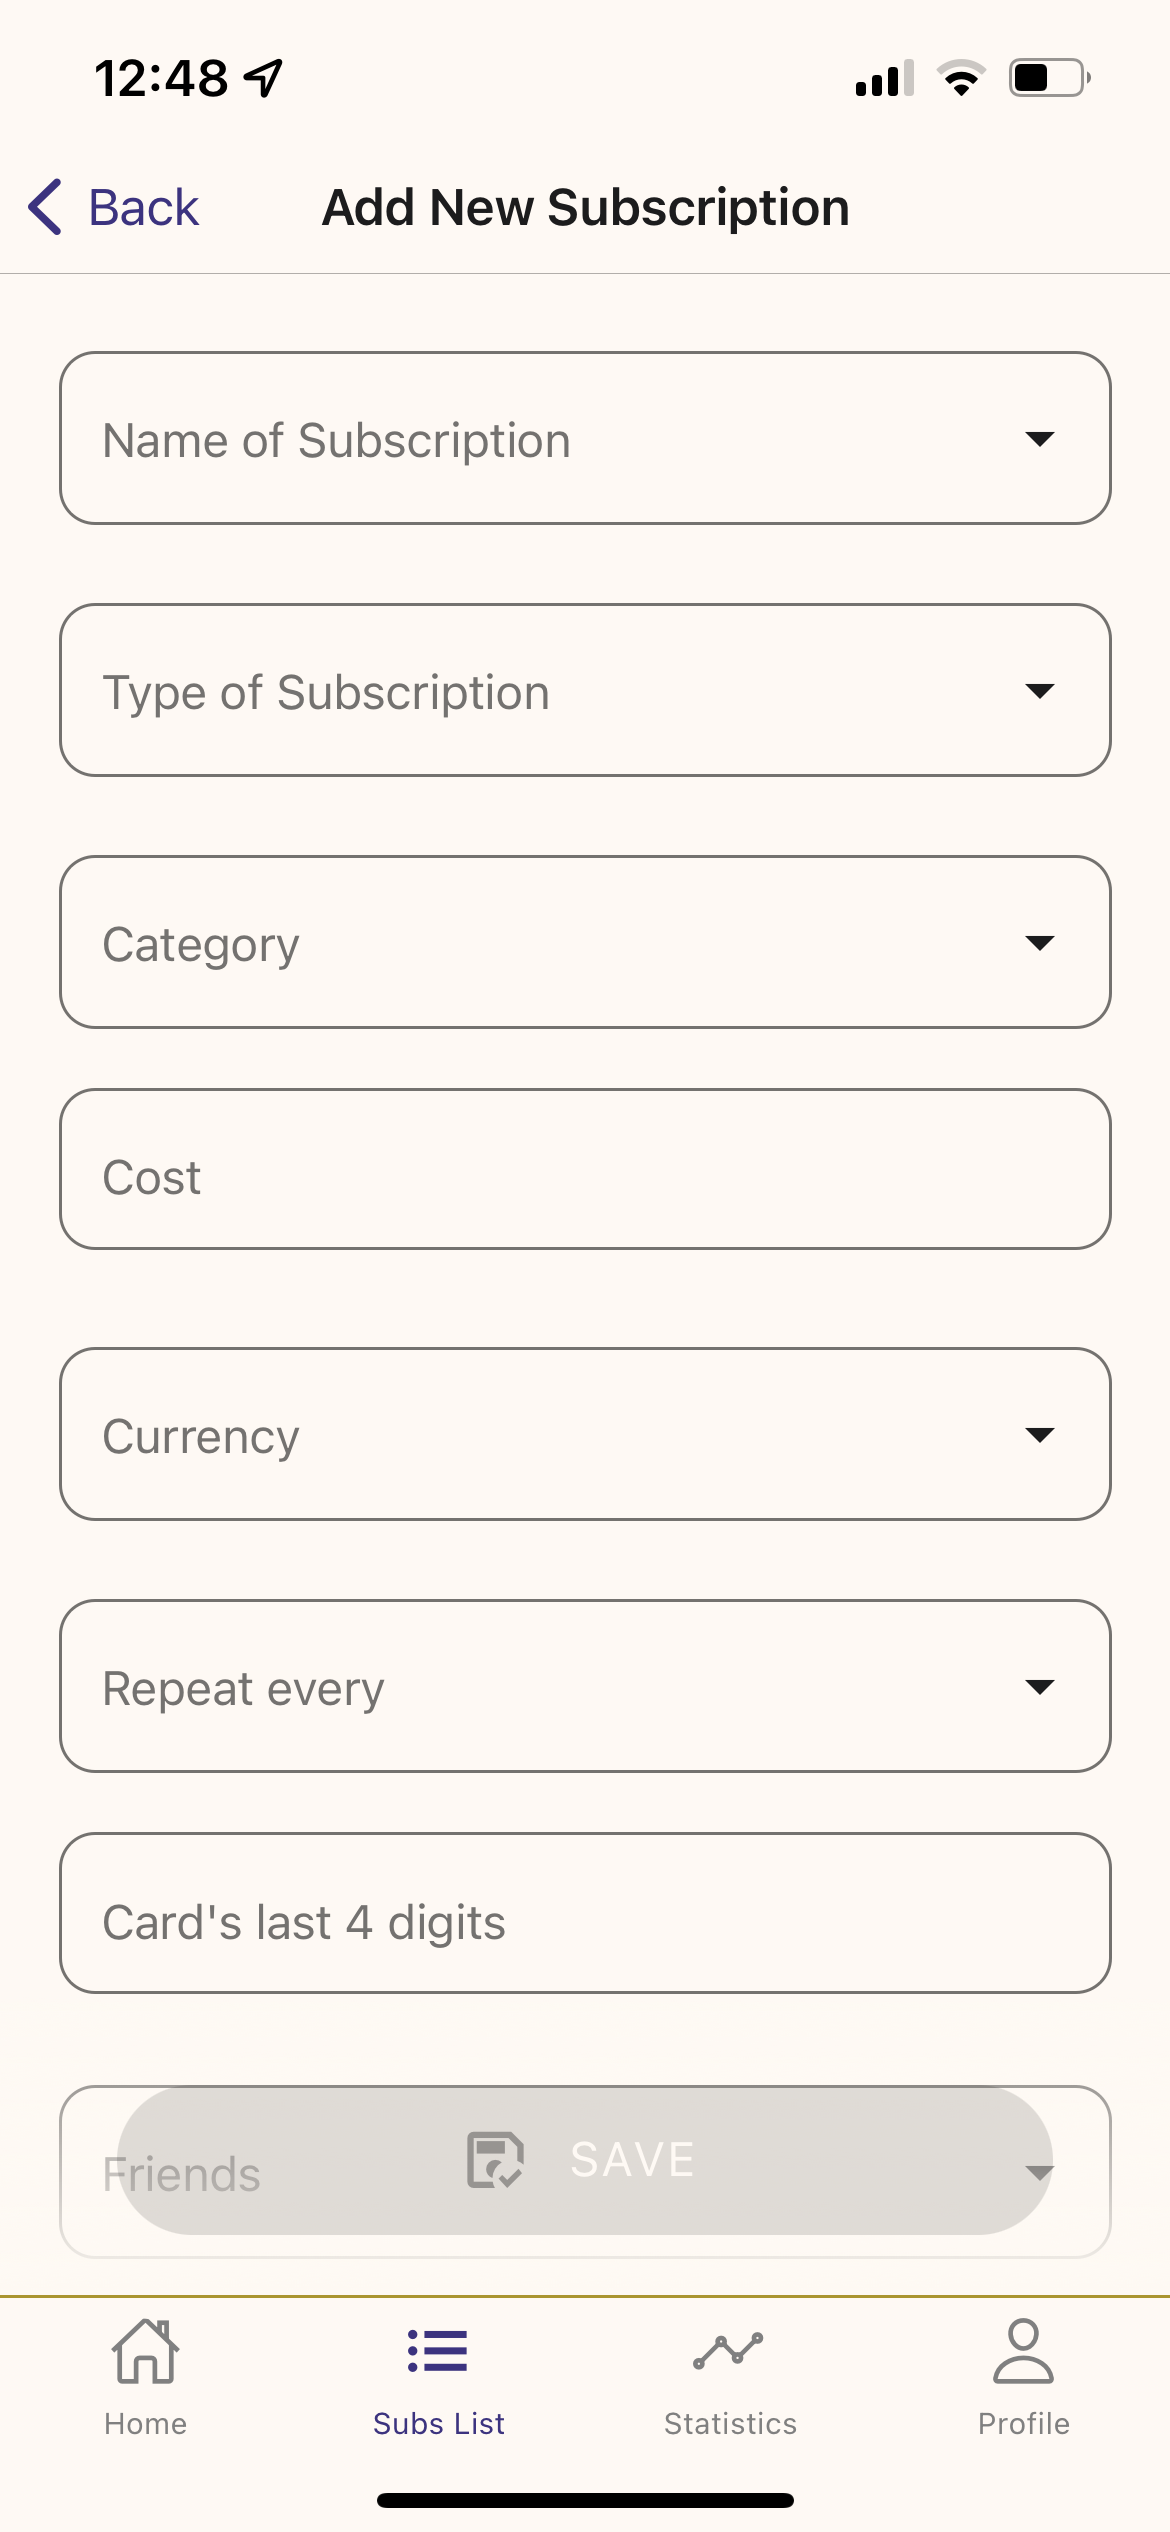
\includegraphics[width=0.6\textwidth, clip]{../../assets/smartphone/add.PNG}
        \caption{Input fields for add form}
        \label{fig:add}
    \end{minipage}
\end{figure}

\begin{figure}[h!]
    \centering
    \begin{minipage}[c]{0.45\textwidth}
        \centering
        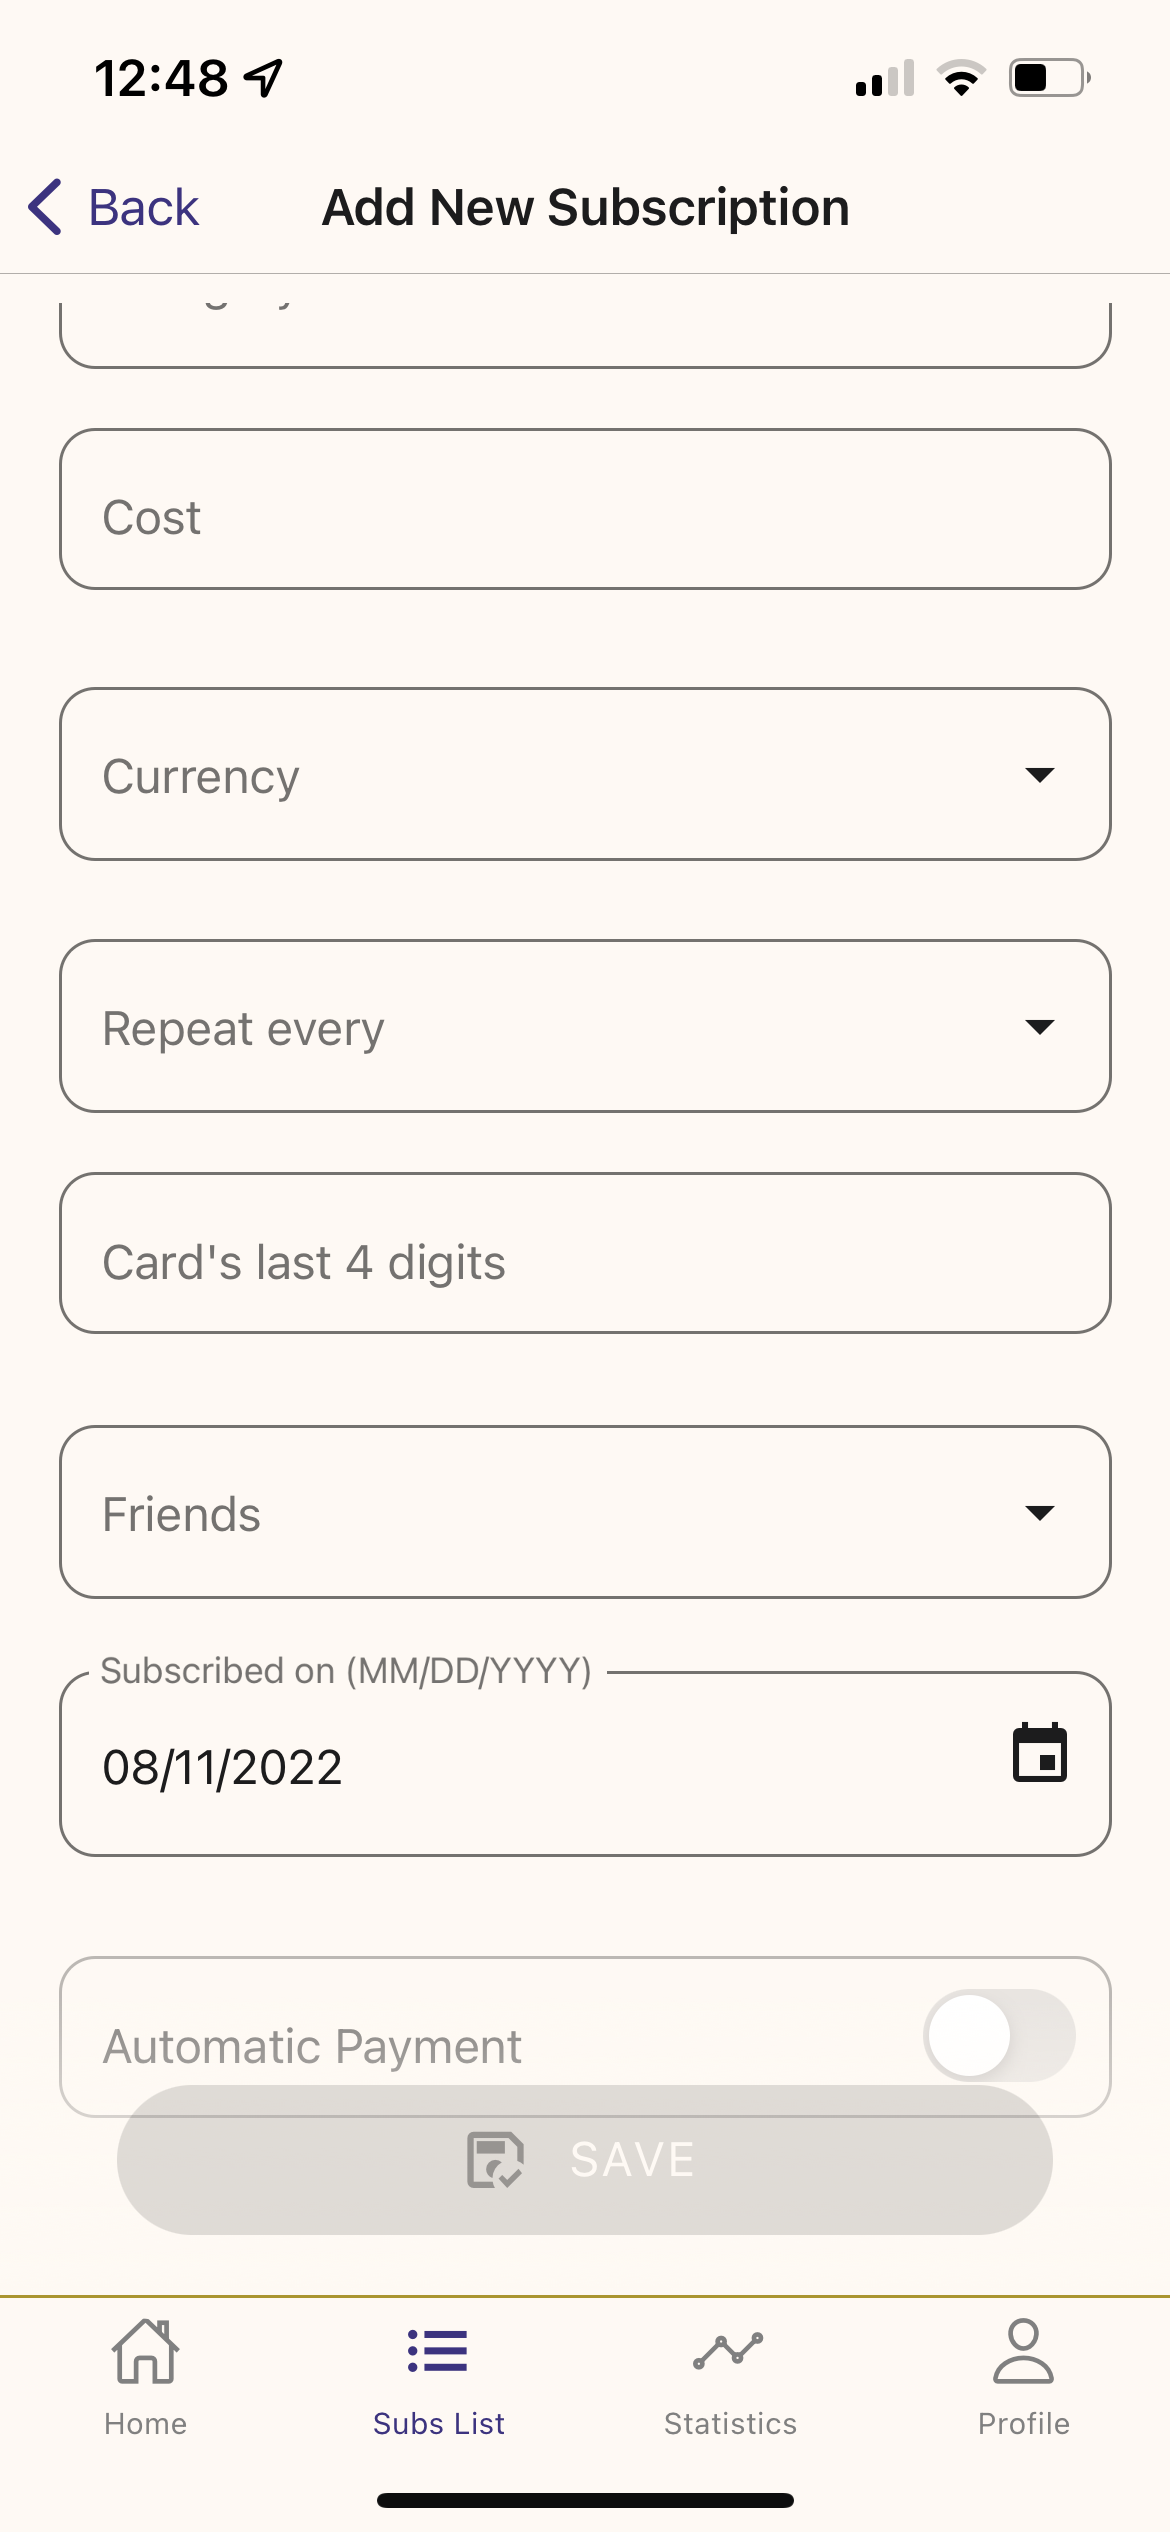
\includegraphics[width=0.6\textwidth, clip]{../../assets/smartphone/add2.PNG}
        \caption{Final fields in add form}
        \label{fig:add2}
    \end{minipage}\hspace{1cm}%
    \begin{minipage}[c]{0.45\textwidth}
        \centering
        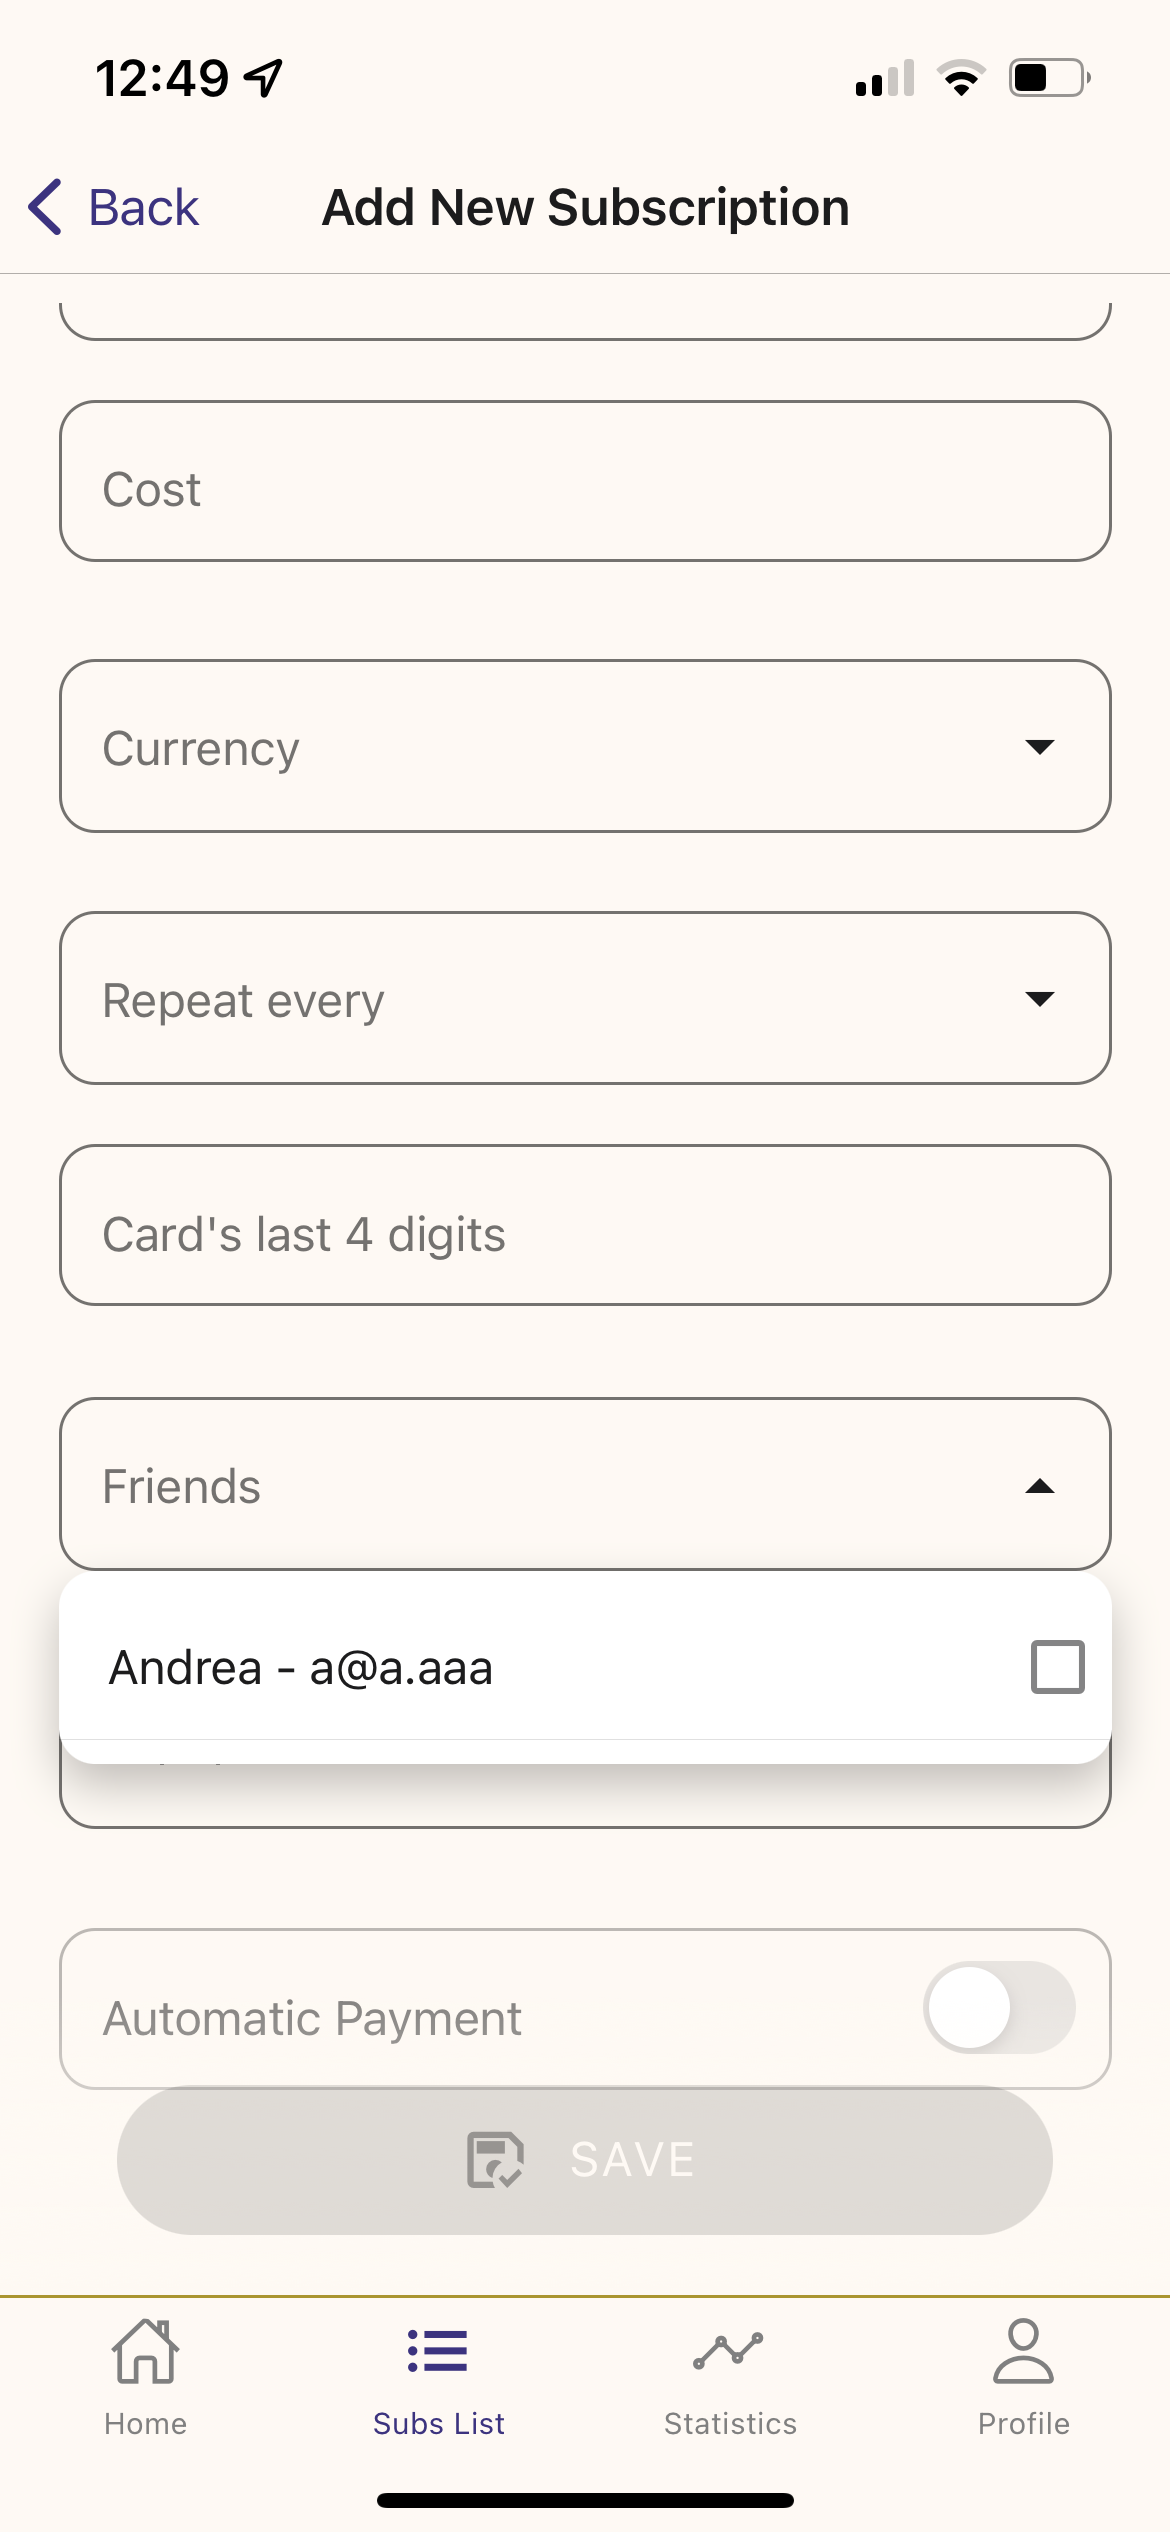
\includegraphics[width=0.6\textwidth, clip]{../../assets/smartphone/addDrop.PNG}
        \caption{Multi-choice drop down menu}
        \label{fig:addDrop}
    \end{minipage}
\end{figure}

\begin{figure}[h!]
    \centering
    \begin{minipage}[c]{0.45\textwidth}
        \centering
        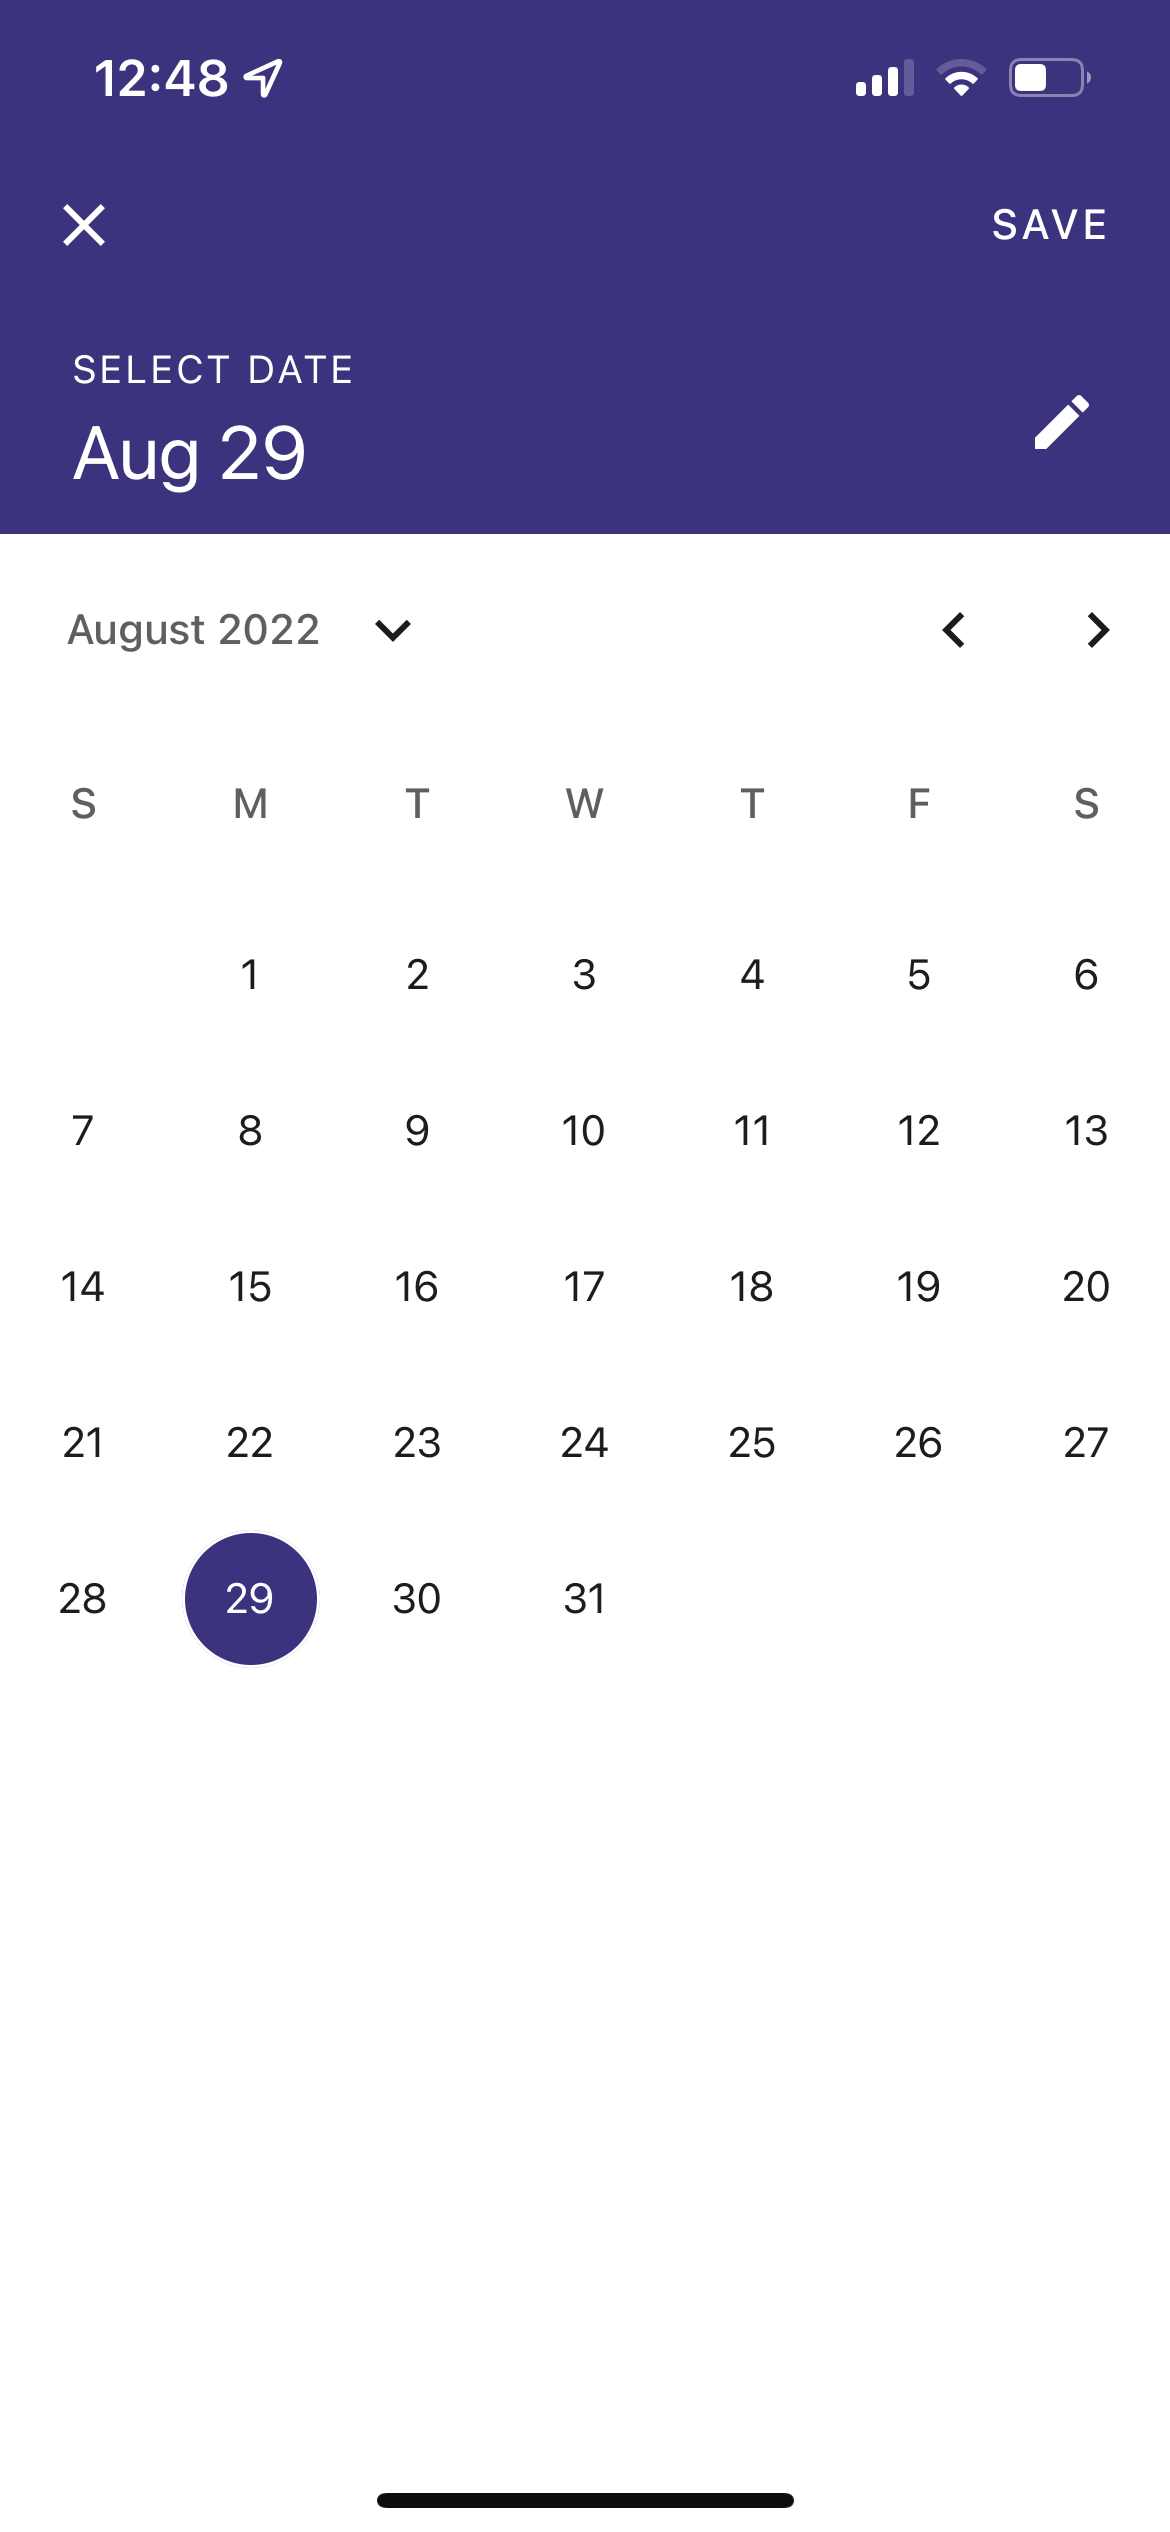
\includegraphics[width=0.6\textwidth, clip]{../../assets/smartphone/calendar.PNG}
        \caption{Calendar page to set subscribed on date}
        \label{fig:calendar}
    \end{minipage}\hspace{1cm}%
    \begin{minipage}[c]{0.45\textwidth}
        \centering
        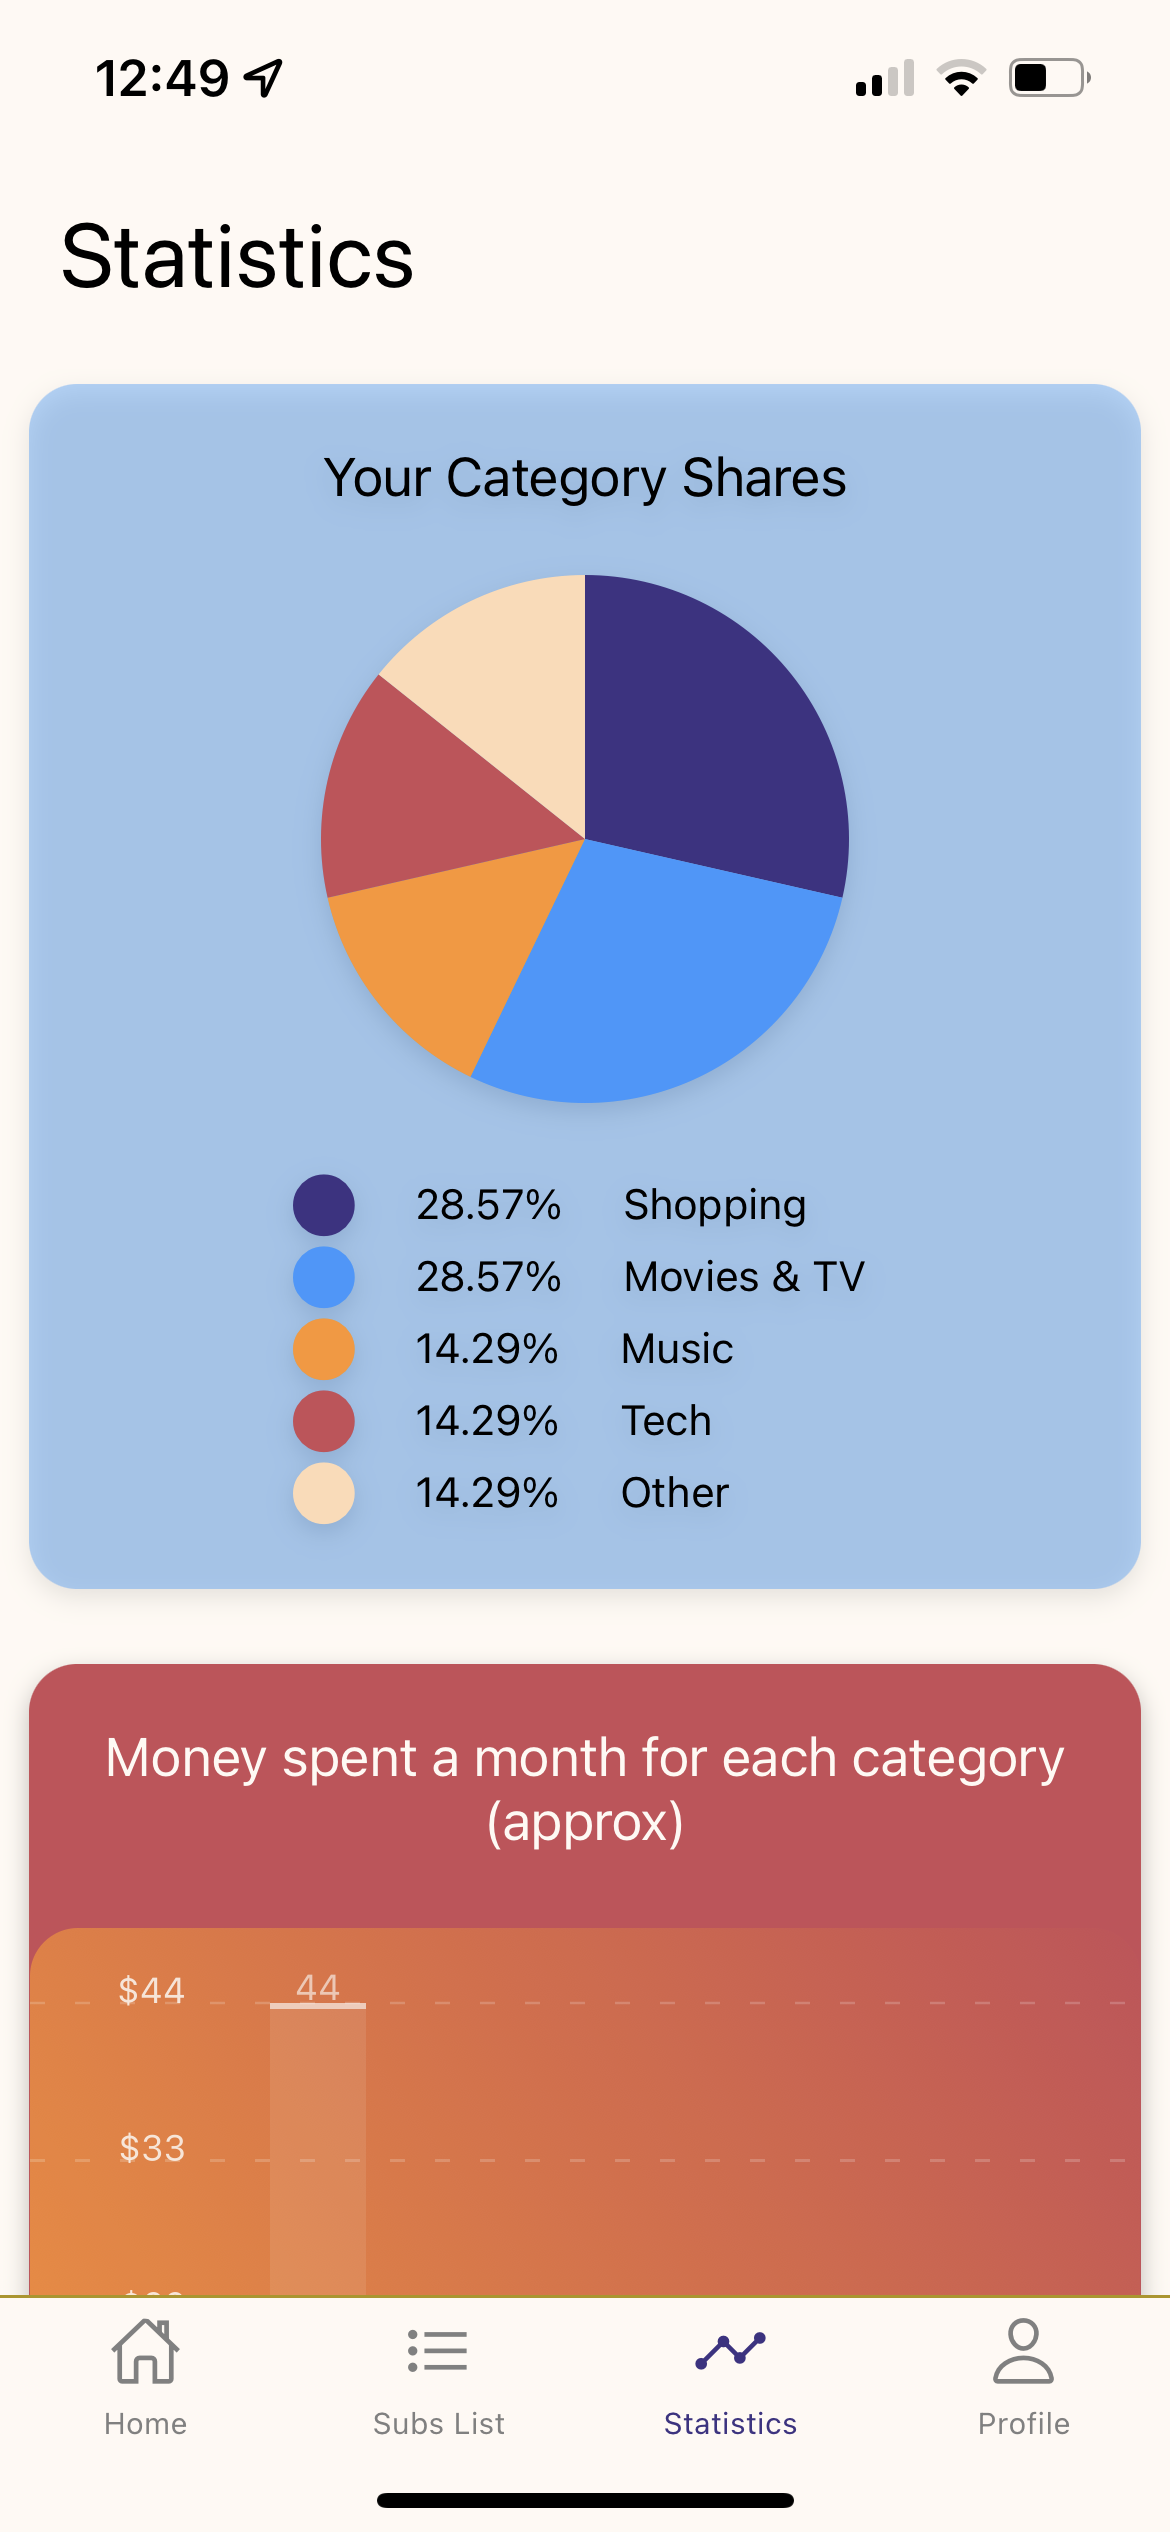
\includegraphics[width=0.6\textwidth, clip]{../../assets/smartphone/stat.PNG}
        \caption{Statistics: pie chart}
        \label{fig:stat}
    \end{minipage}
\end{figure}

\begin{figure}[h!]
    \centering
    \begin{minipage}[c]{0.45\textwidth}
        \centering
        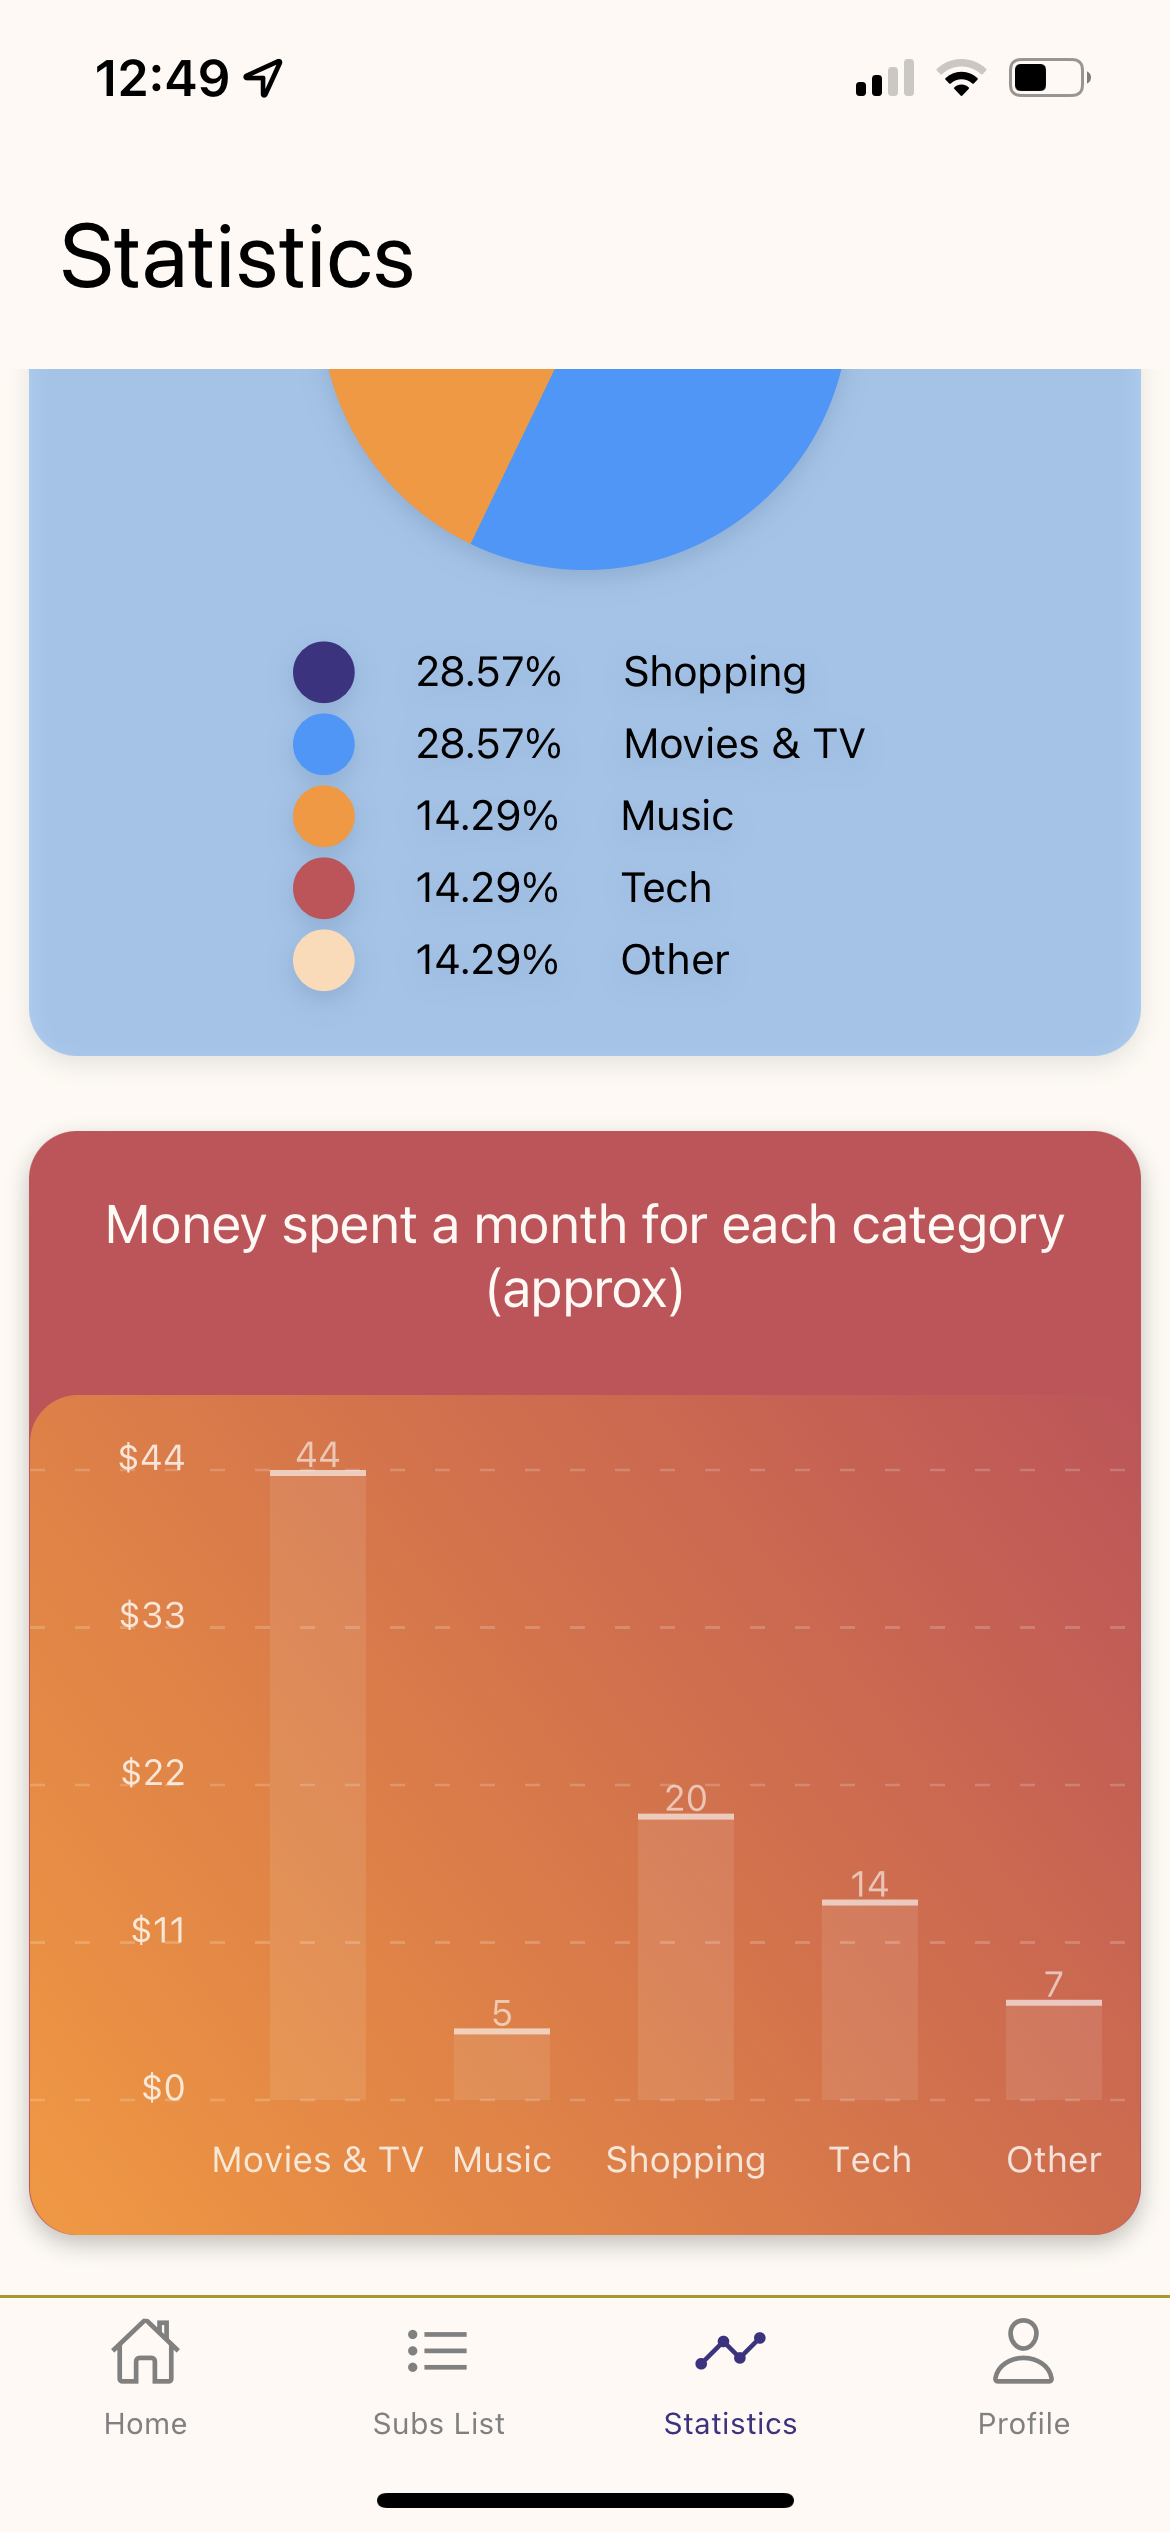
\includegraphics[width=0.6\textwidth, clip]{../../assets/smartphone/stat2.PNG}
        \caption{Statistics: bar chart}
        \label{fig:stat2}
    \end{minipage}\hspace{1cm}%
    \begin{minipage}[c]{0.45\textwidth}
        \centering
        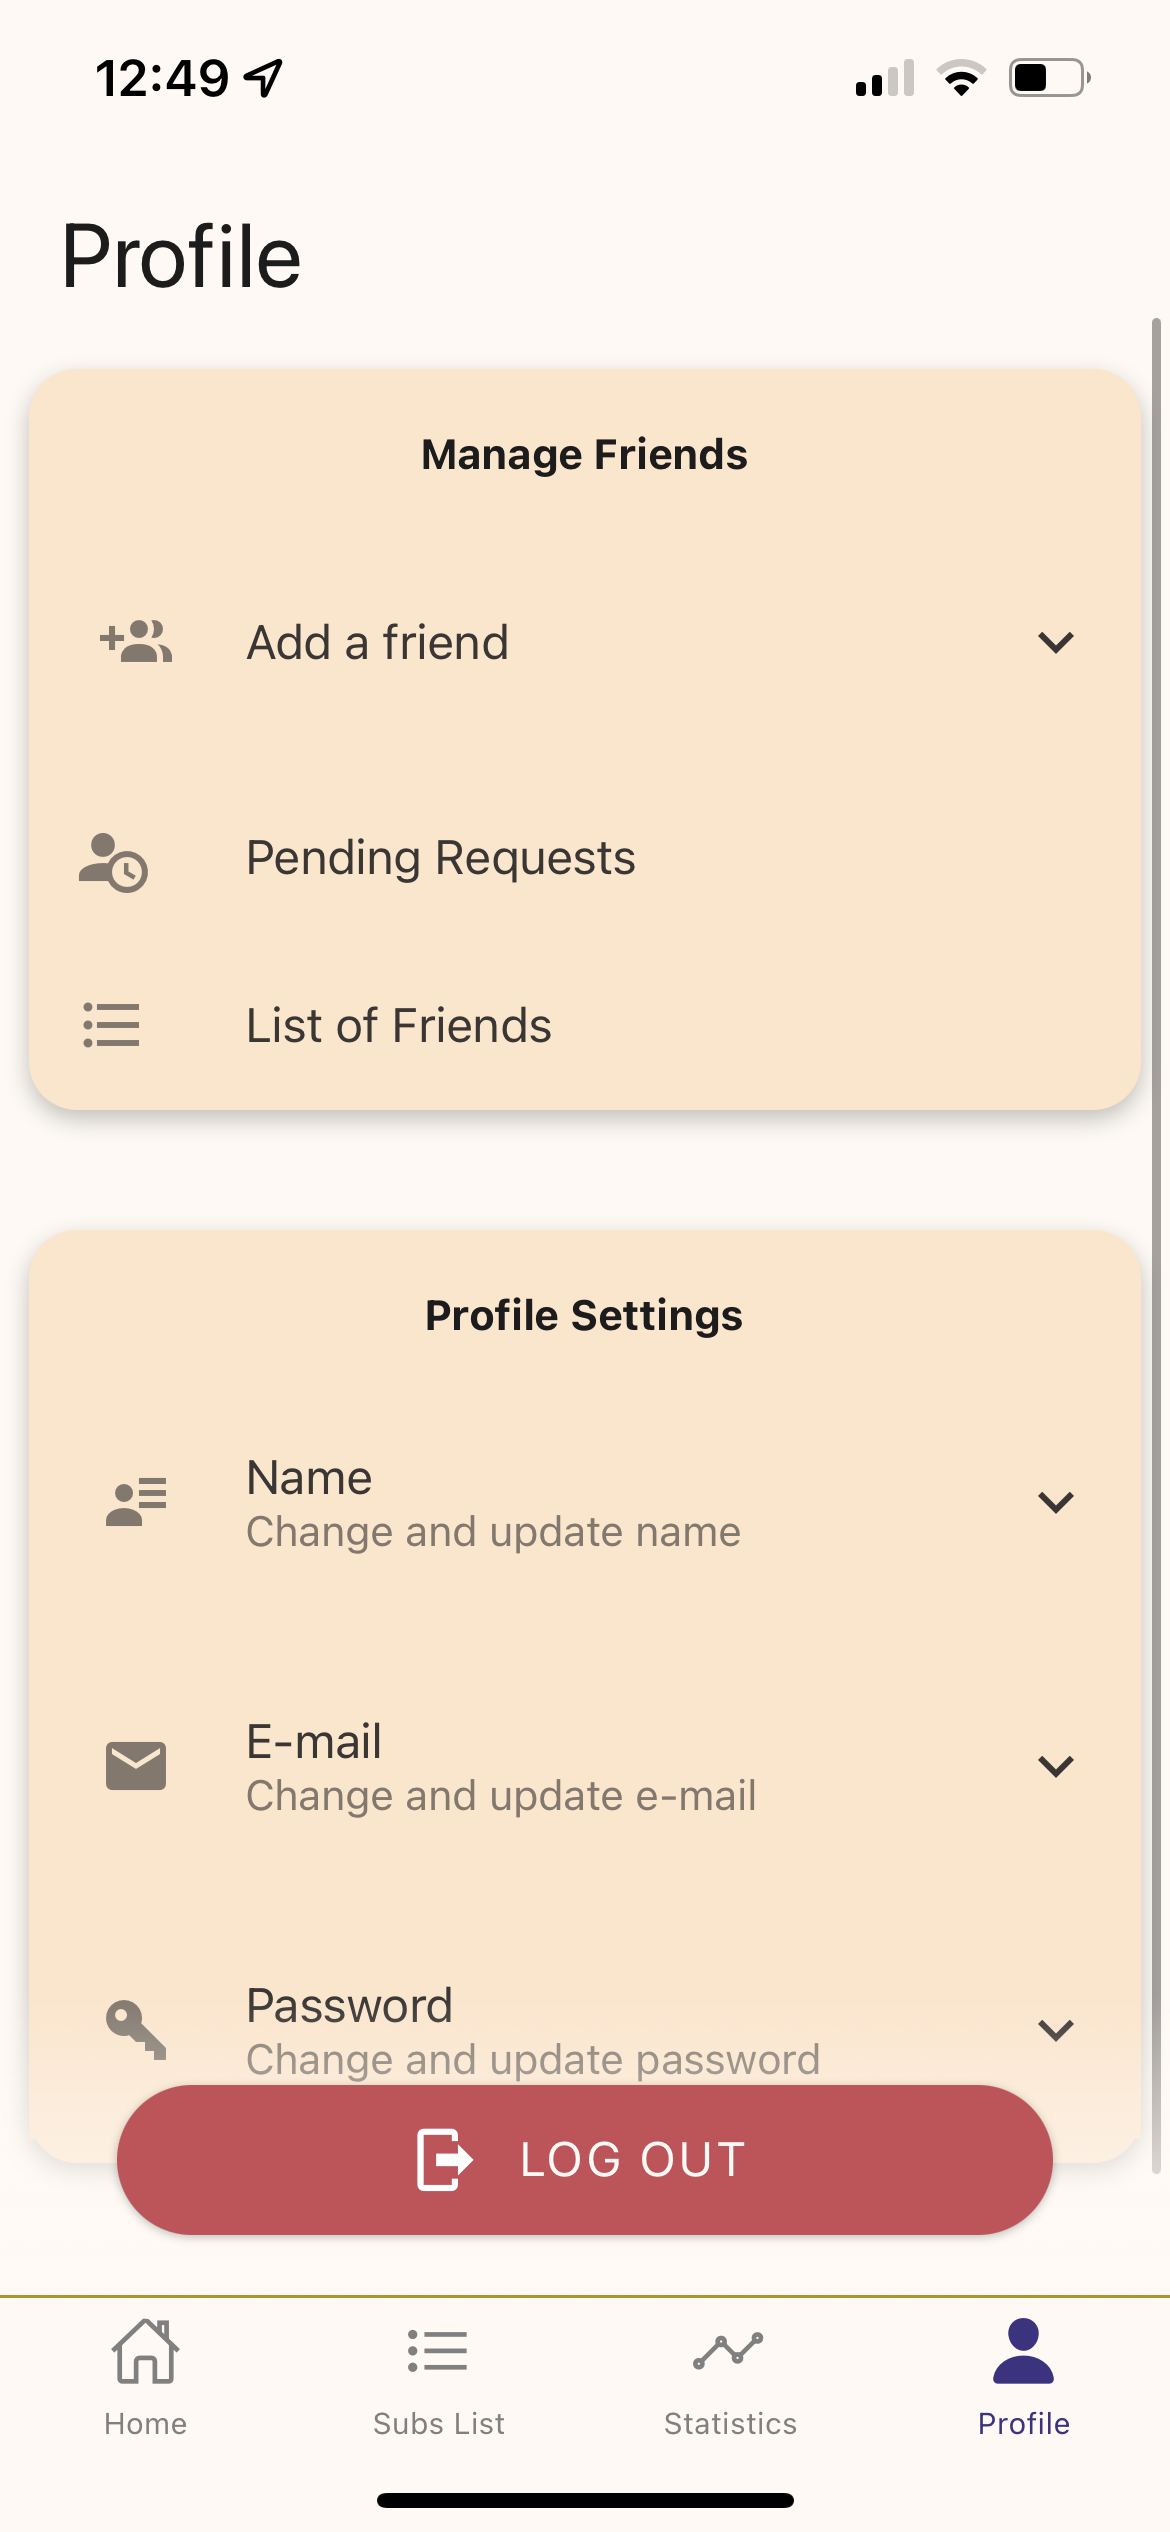
\includegraphics[width=0.6\textwidth, clip]{../../assets/smartphone/profile.PNG}
        \caption{Profile page: manage friends and settings}
        \label{fig:profile}
    \end{minipage}
\end{figure}

\begin{figure}[h!]
    \centering
    \begin{minipage}[c]{0.45\textwidth}
        \centering
        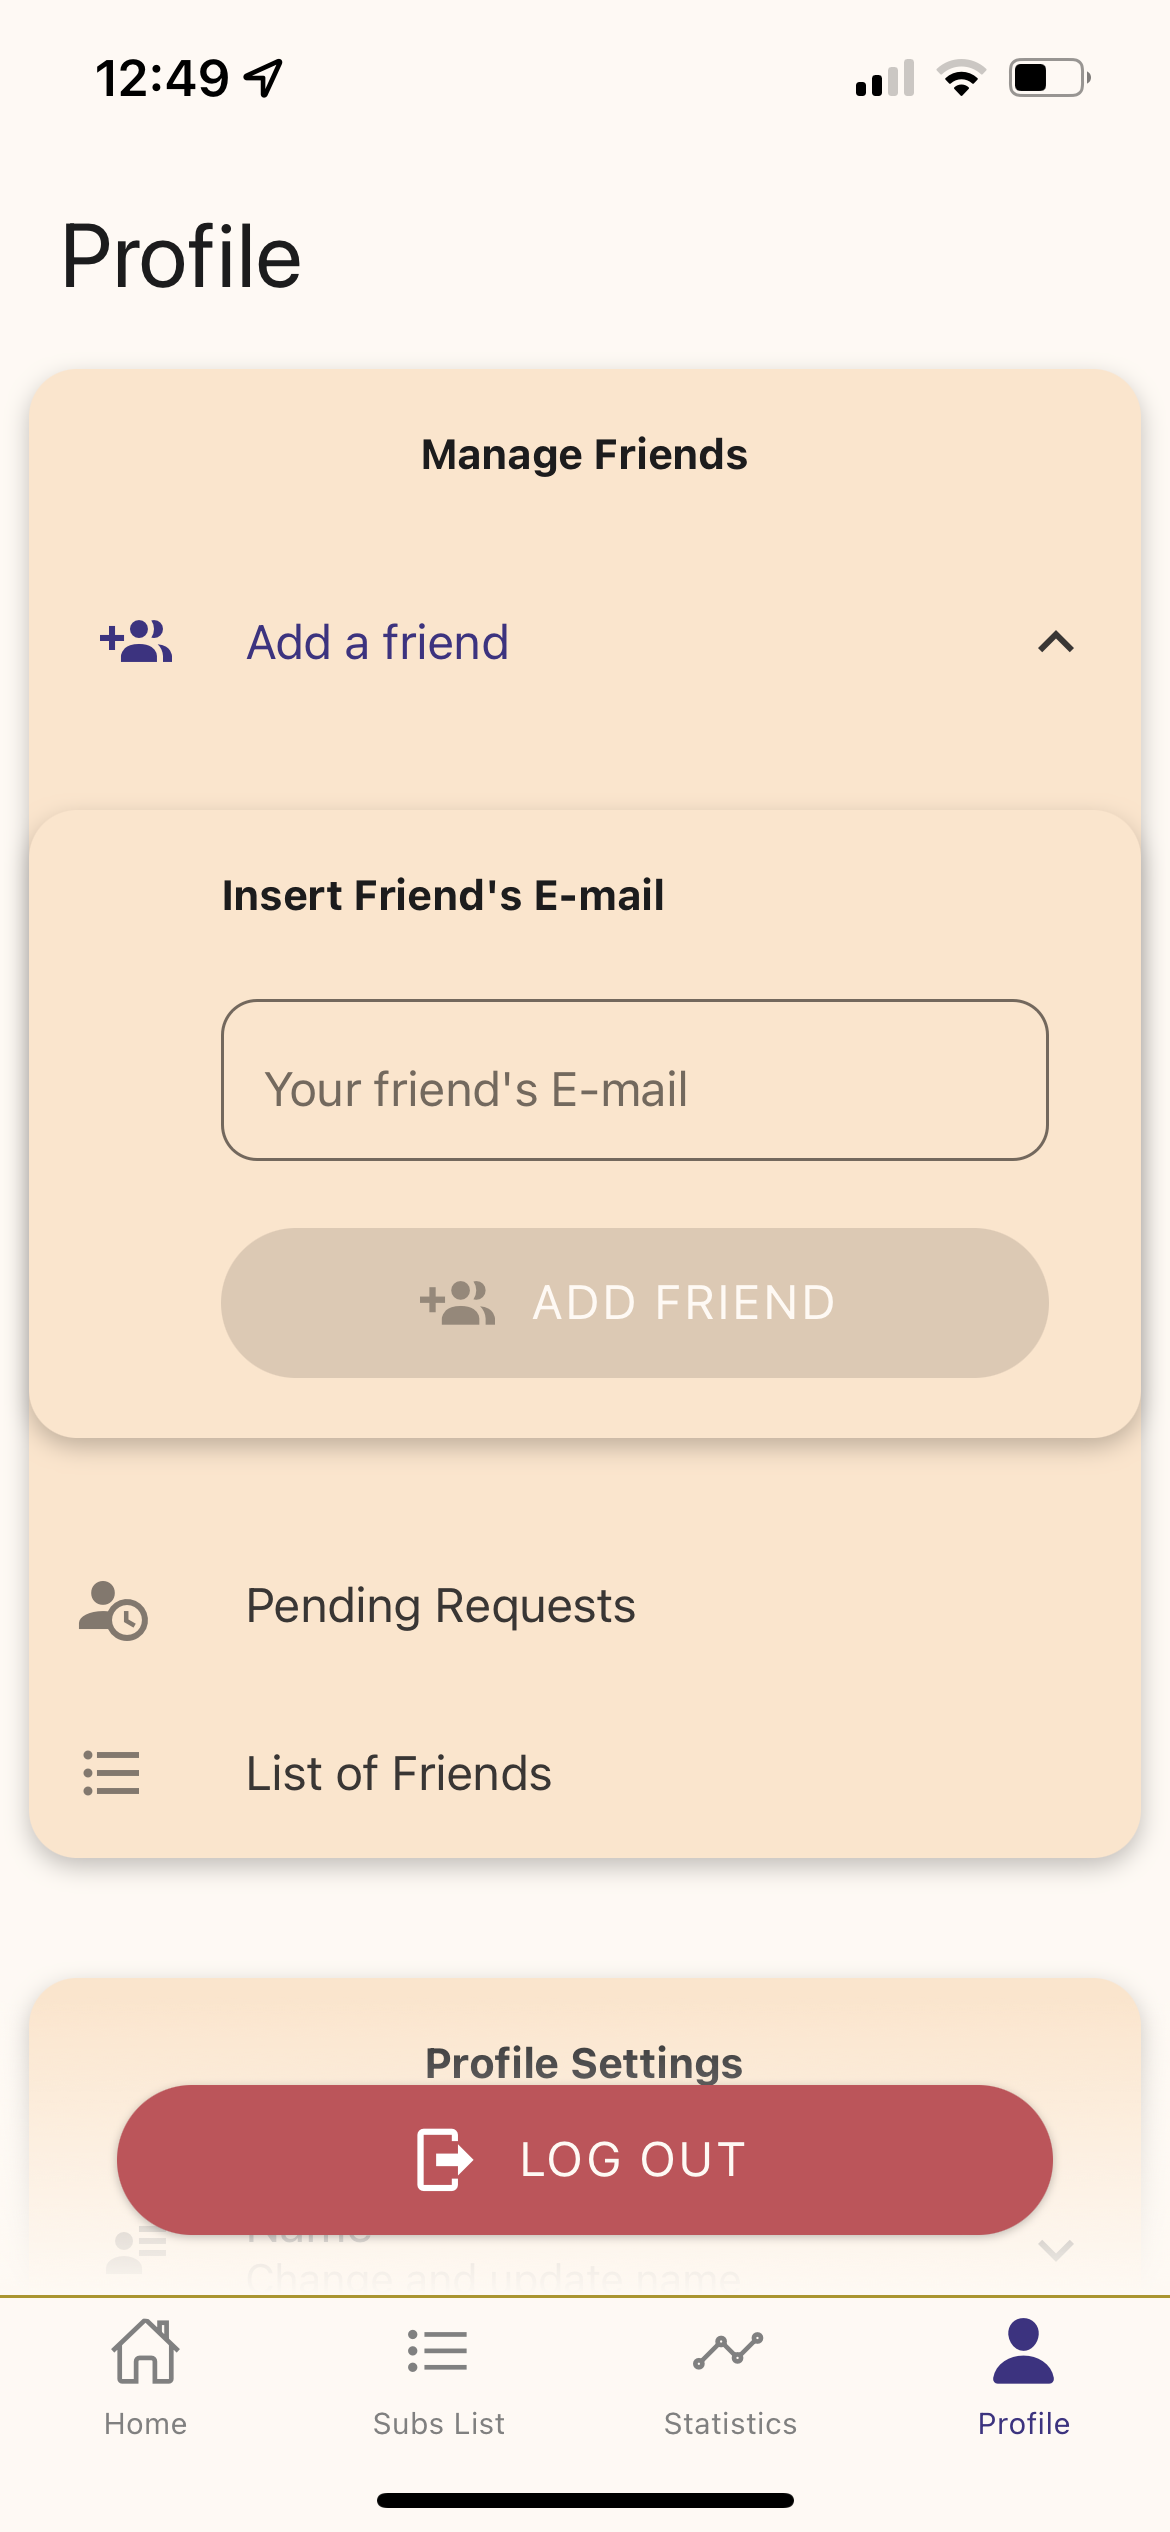
\includegraphics[width=0.6\textwidth, clip]{../../assets/smartphone/profileAdd.PNG}
        \caption{Add friend input field}
        \label{fig:profileAdd}
    \end{minipage}\hspace{1cm}%
    \begin{minipage}[c]{0.45\textwidth}
        \centering
        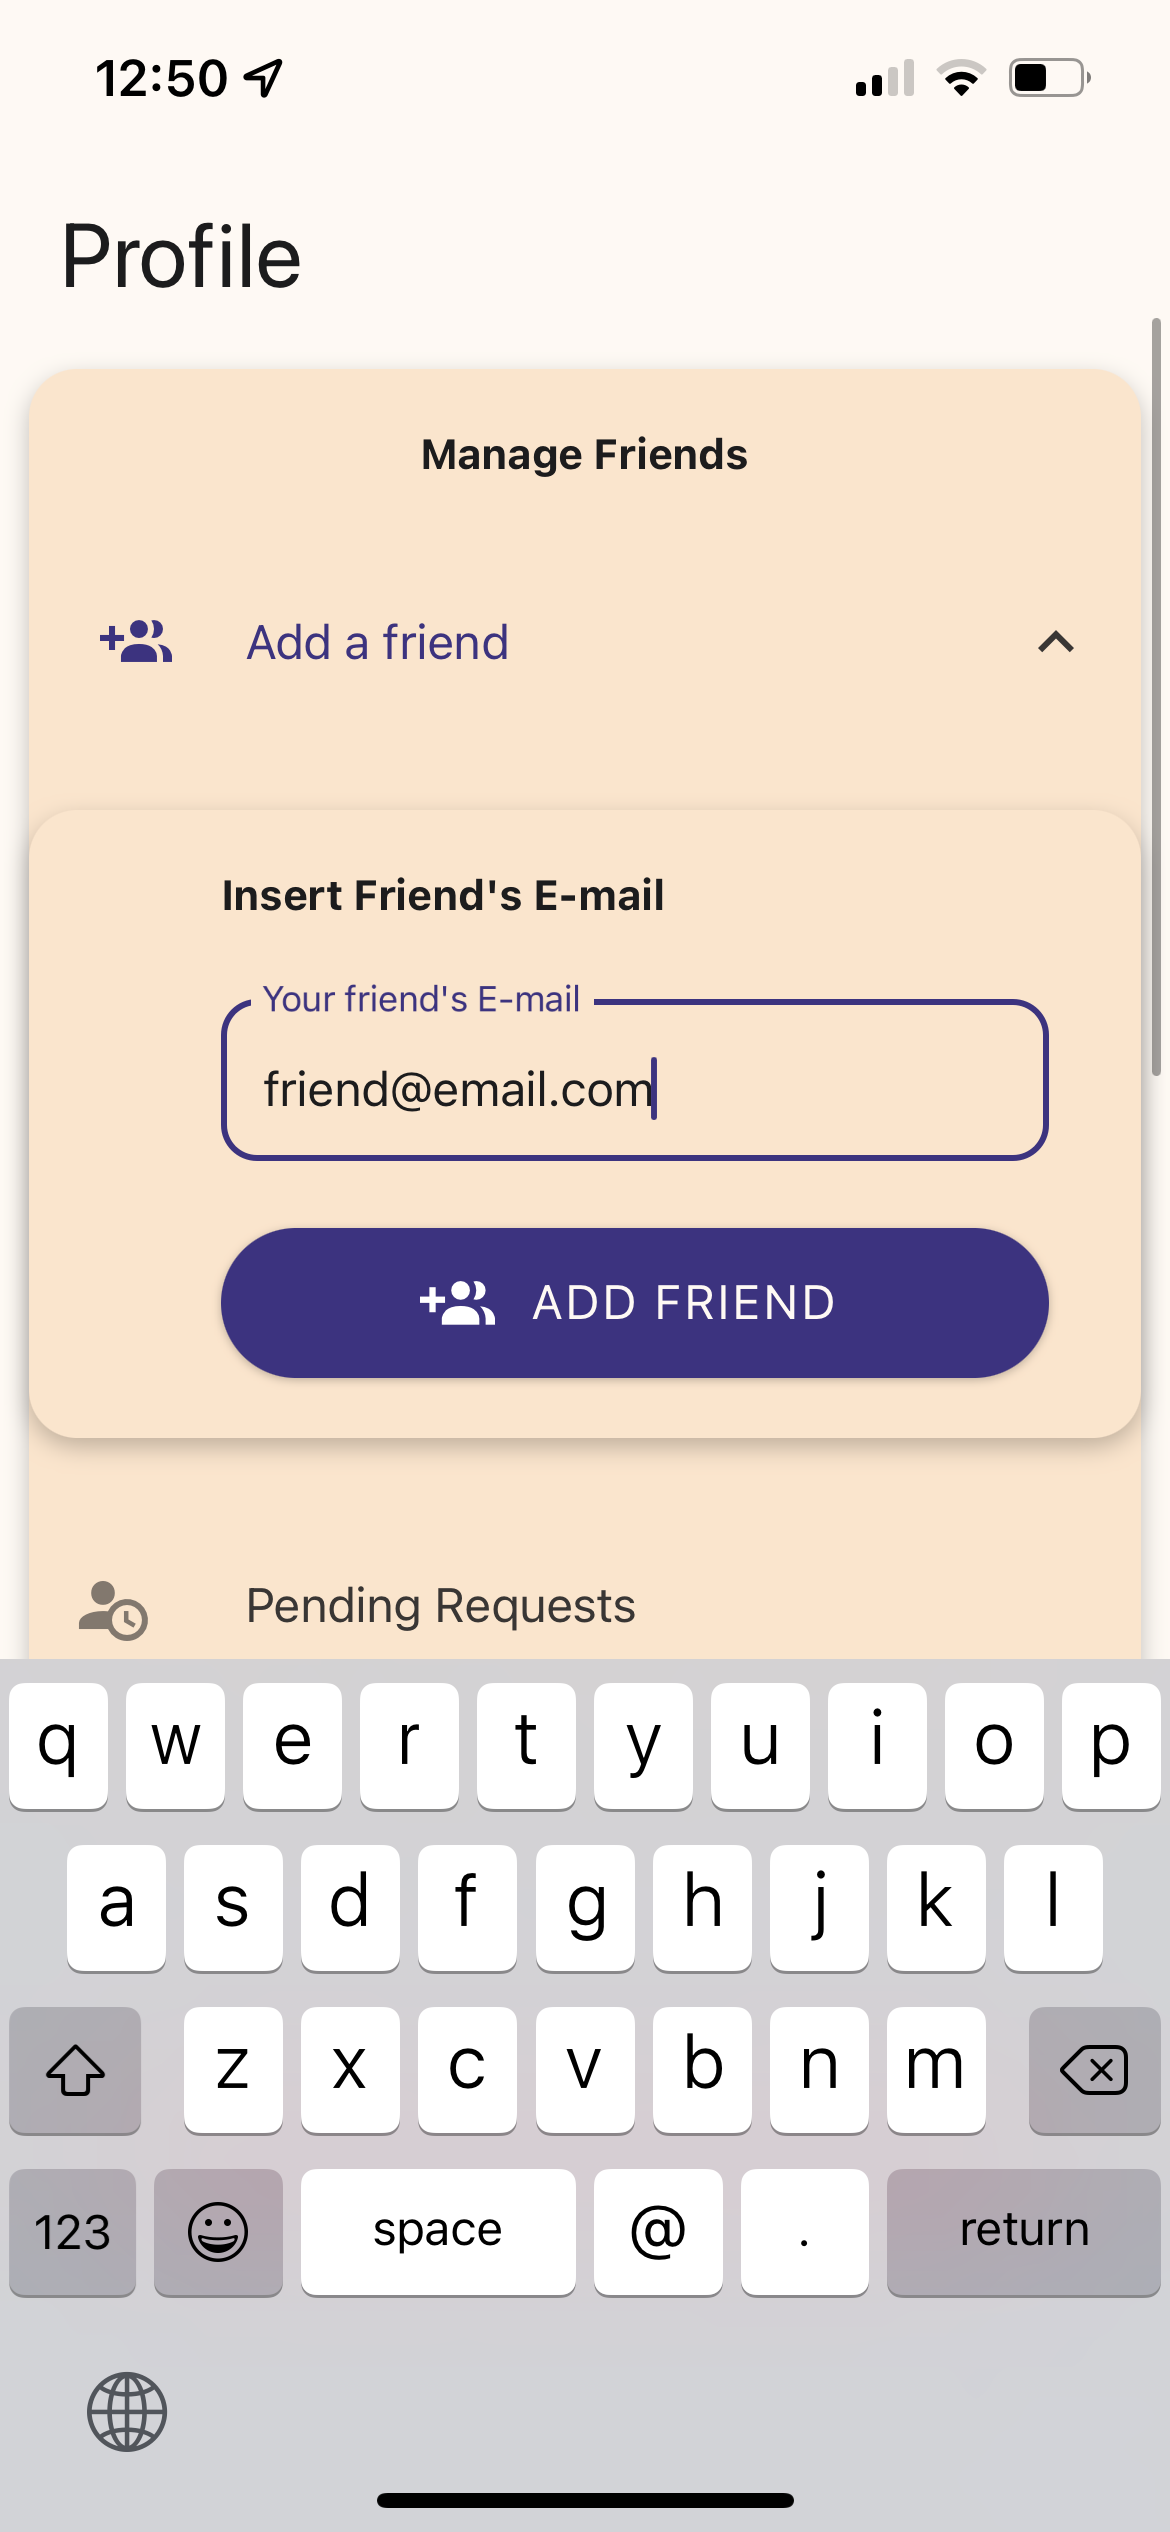
\includegraphics[width=0.6\textwidth, clip]{../../assets/smartphone/profileAddEmail.PNG}
        \caption{When the inserted e-mail has a valid format, the button is enabled}
        \label{fig:profileAddEmail}
    \end{minipage}
\end{figure}

\begin{figure}[h!]
    \centering
    \begin{minipage}[c]{0.45\textwidth}
        \centering
        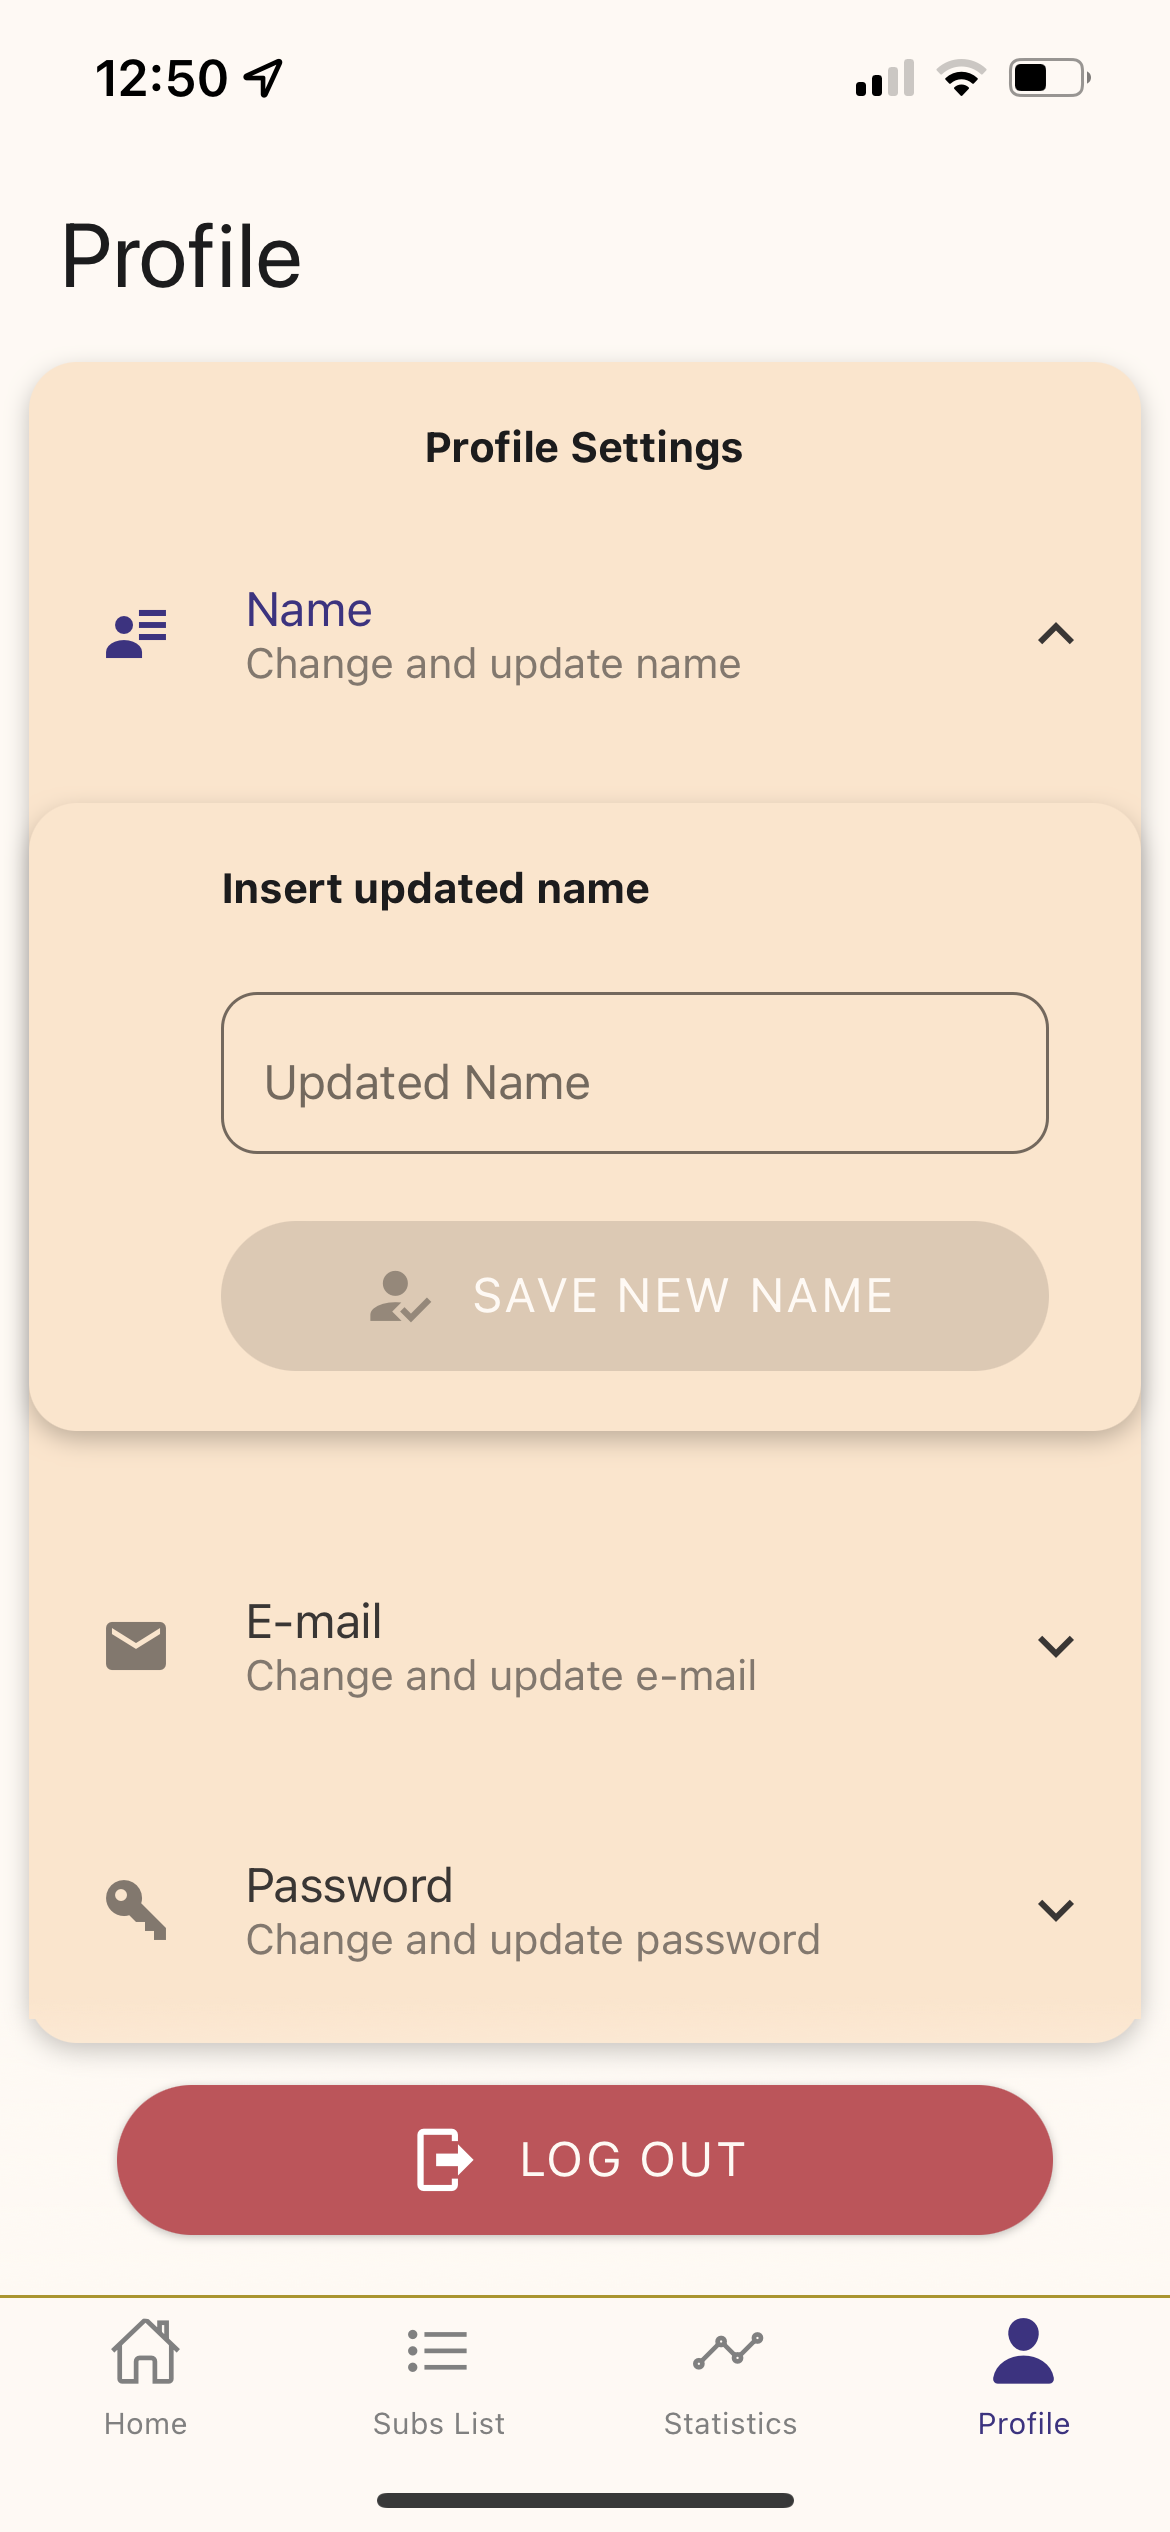
\includegraphics[width=0.6\textwidth, clip]{../../assets/smartphone/profileNewName.PNG}
        \caption{Update name}
        \label{fig:profileNewName}
    \end{minipage}\hspace{1cm}%
    \begin{minipage}[c]{0.45\textwidth}
        \centering
        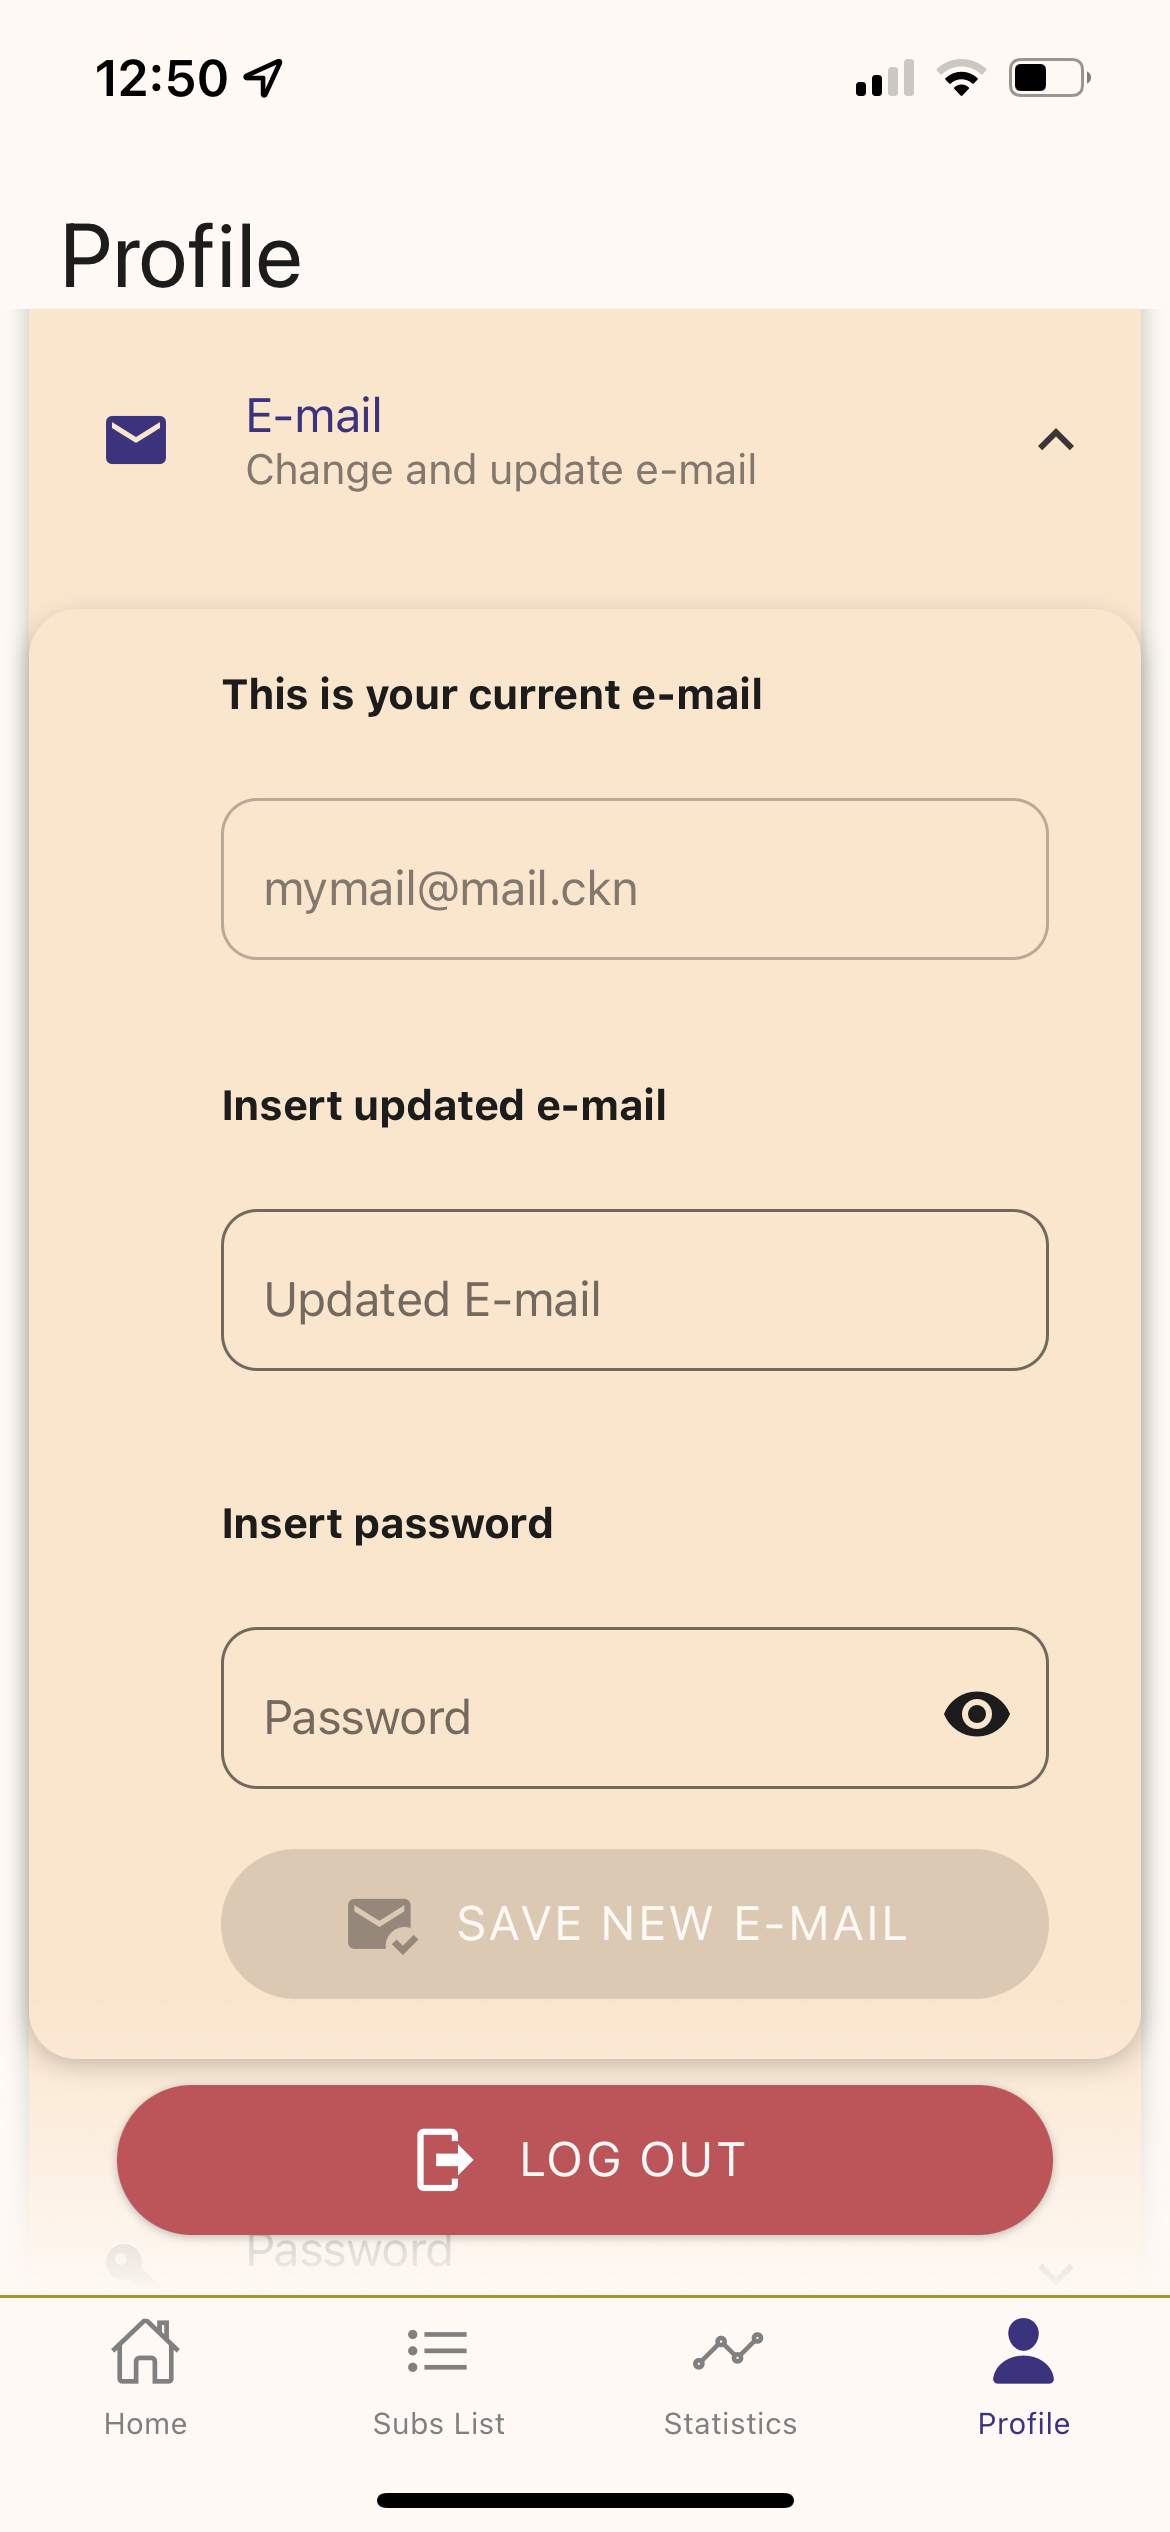
\includegraphics[width=0.6\textwidth, clip]{../../assets/smartphone/profileNewMail.PNG}
        \caption{Update e-mail, upon password insertion}
        \label{fig:profileNewMail}
    \end{minipage}
\end{figure}

\begin{figure}[h!]
    \centering
    \begin{minipage}[c]{0.45\textwidth}
        \centering
        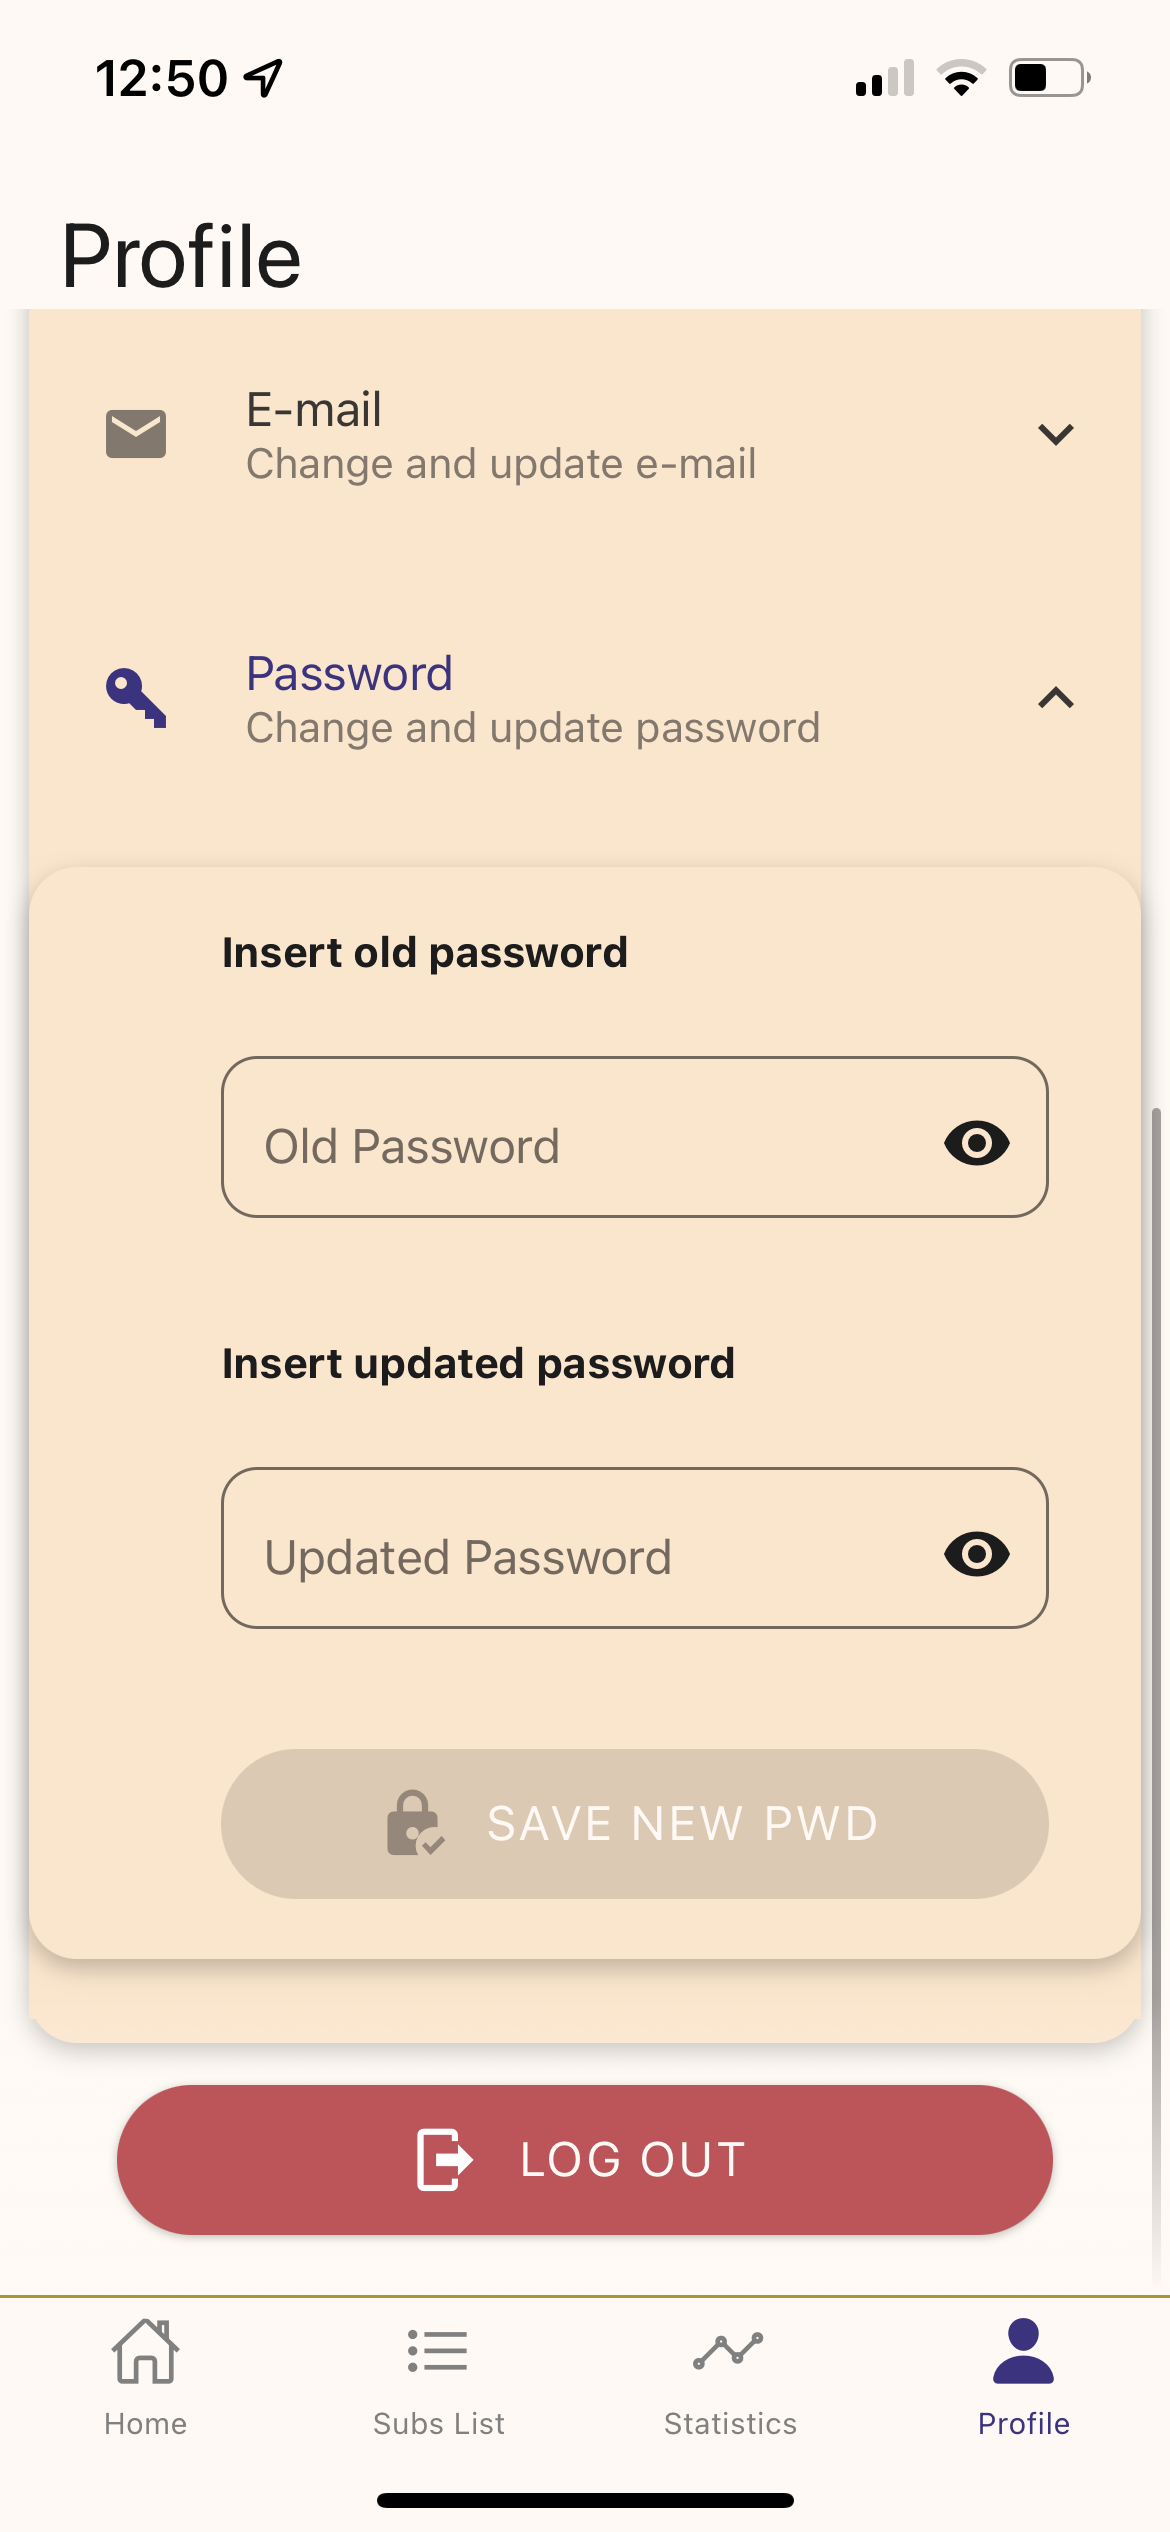
\includegraphics[width=0.6\textwidth, clip]{../../assets/smartphone/profileNewPwd.PNG}
        \caption{Update password, upon old password insertion}
        \label{fig:profileNewPwd}
    \end{minipage}\hspace{1cm}%
    \begin{minipage}[c]{0.45\textwidth}
        \centering
        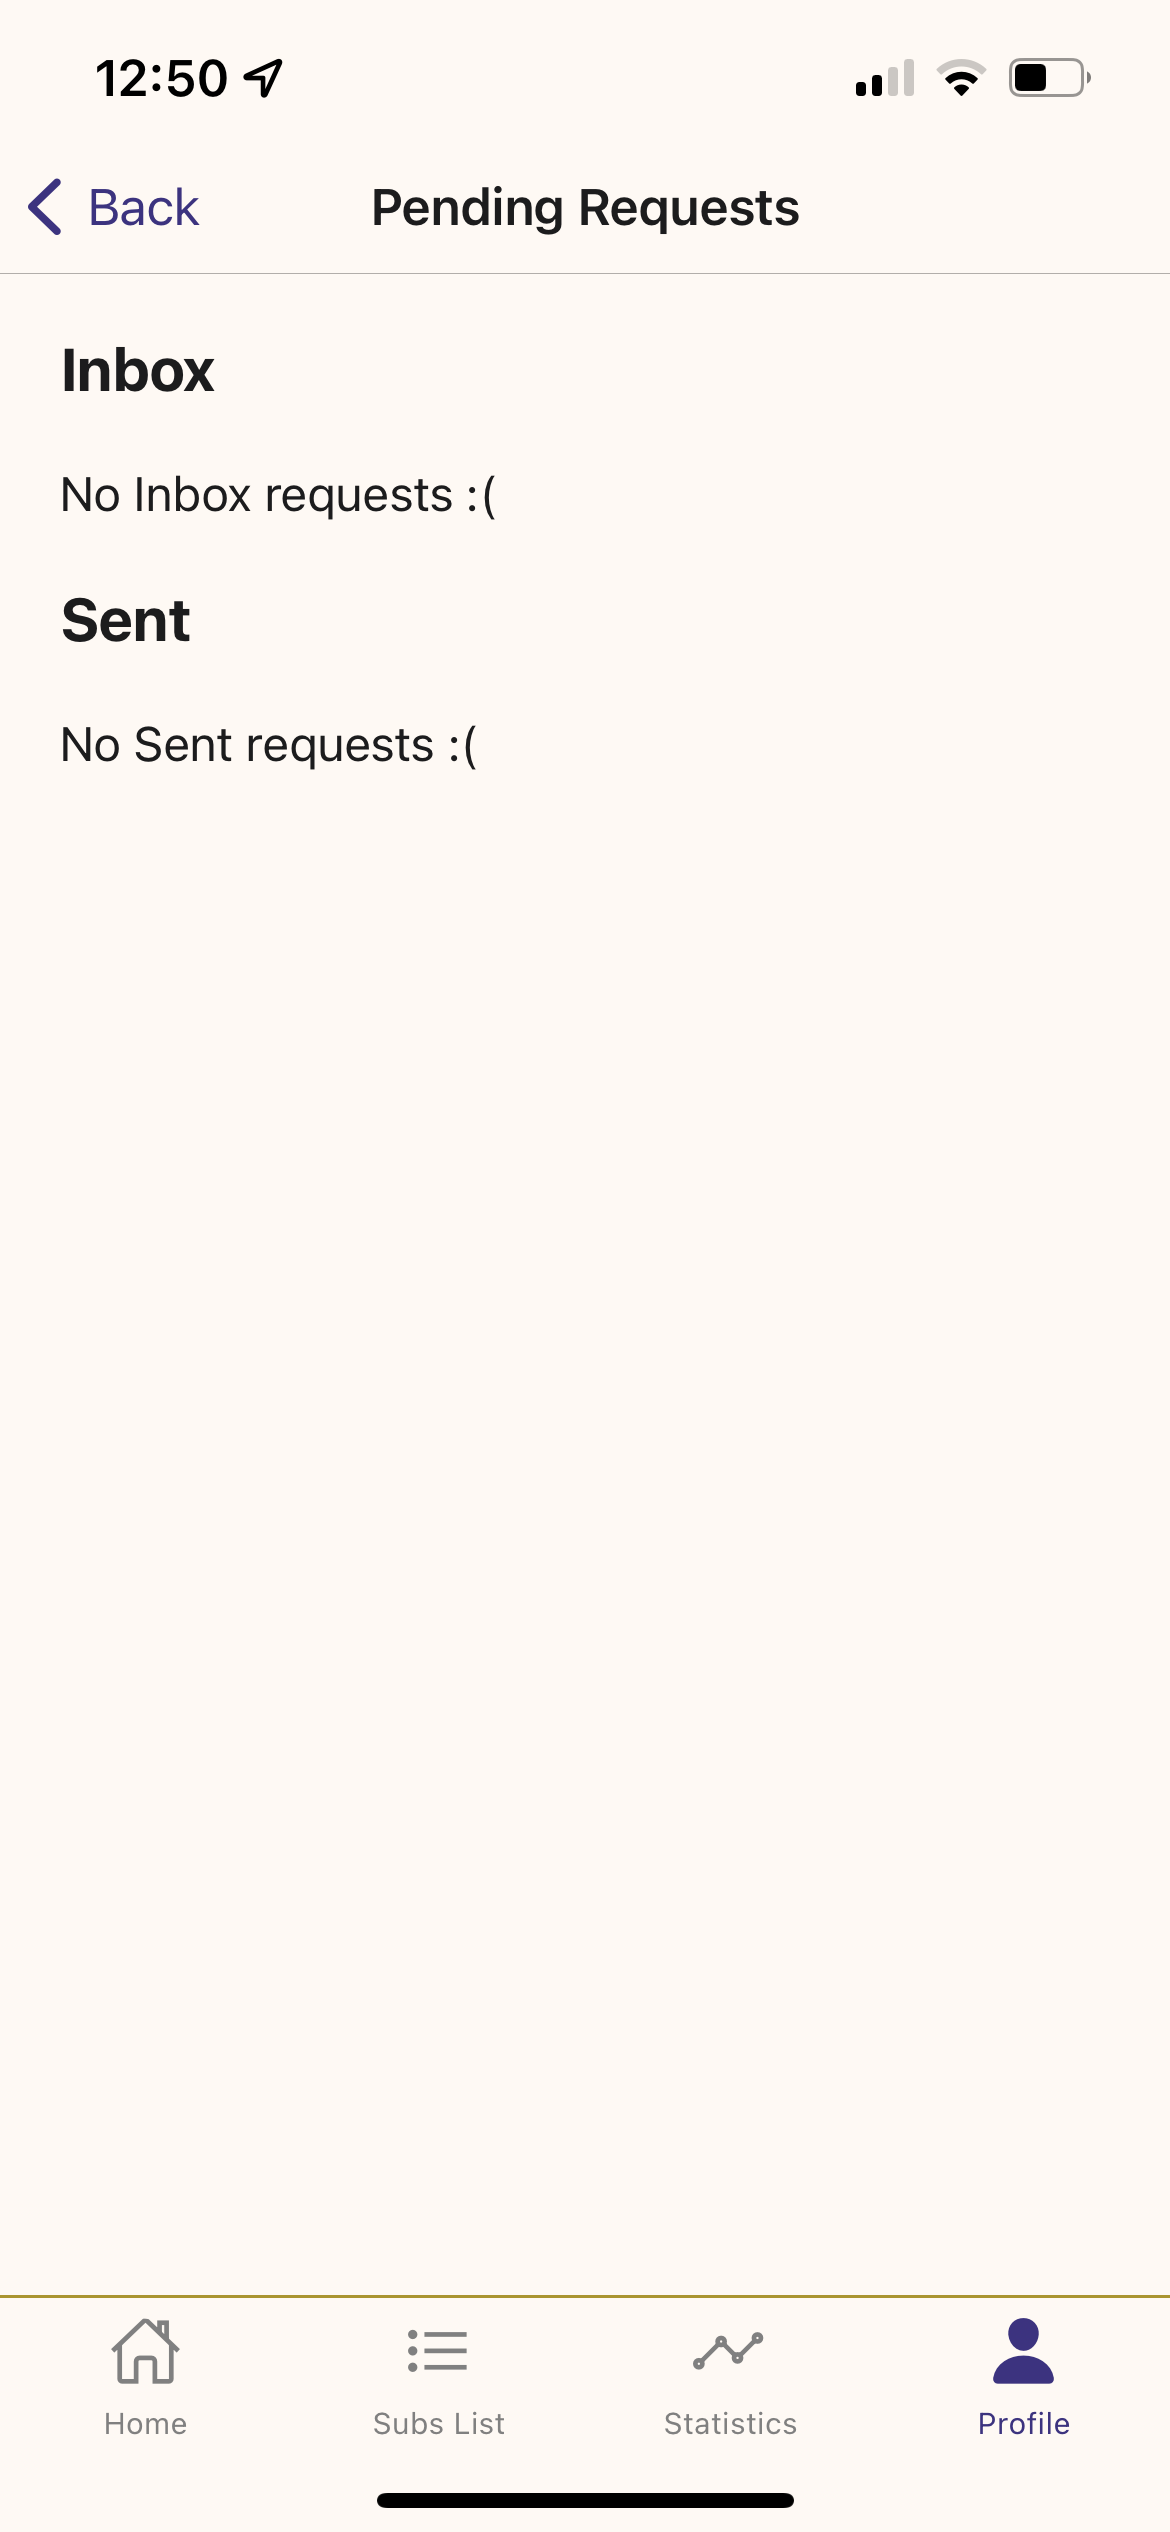
\includegraphics[width=0.6\textwidth, clip]{../../assets/smartphone/pending.PNG}
        \caption{No pending friends requests}
        \label{fig:pending}
    \end{minipage}
\end{figure}

\begin{figure}[h!]
    \centering
    \begin{minipage}[c]{0.45\textwidth}
        \centering
        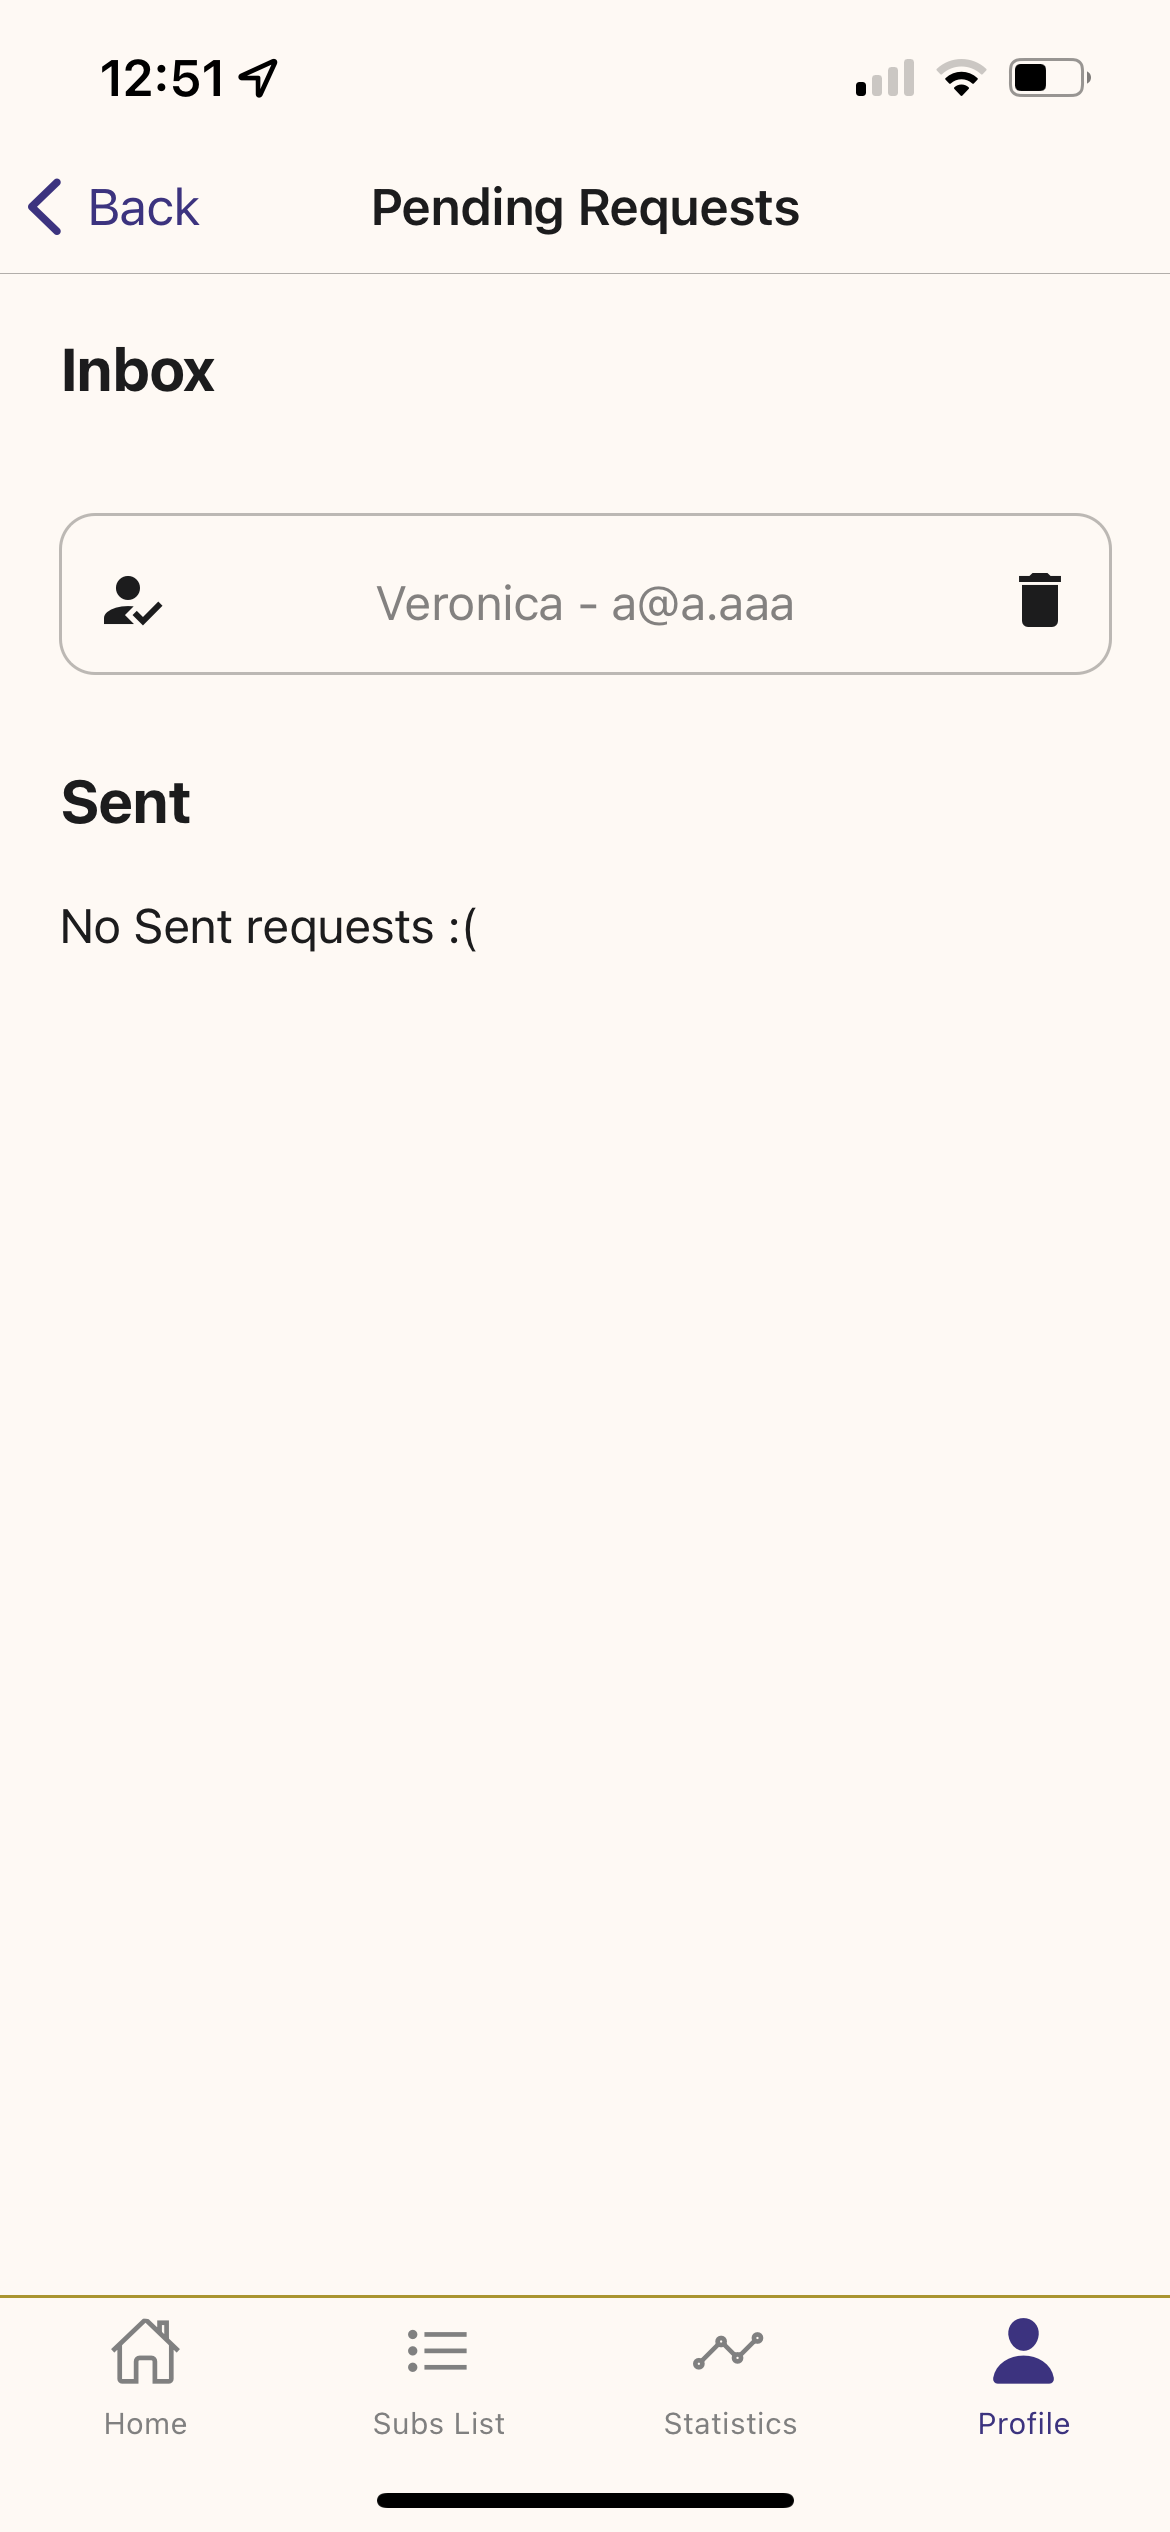
\includegraphics[width=0.6\textwidth, clip]{../../assets/smartphone/pendingIn.PNG}
        \caption{Pending request in inbox: can be accepted or deleted}
        \label{fig:pendingIn}
    \end{minipage}\hspace{1cm}%
    \begin{minipage}[c]{0.45\textwidth}
        \centering
        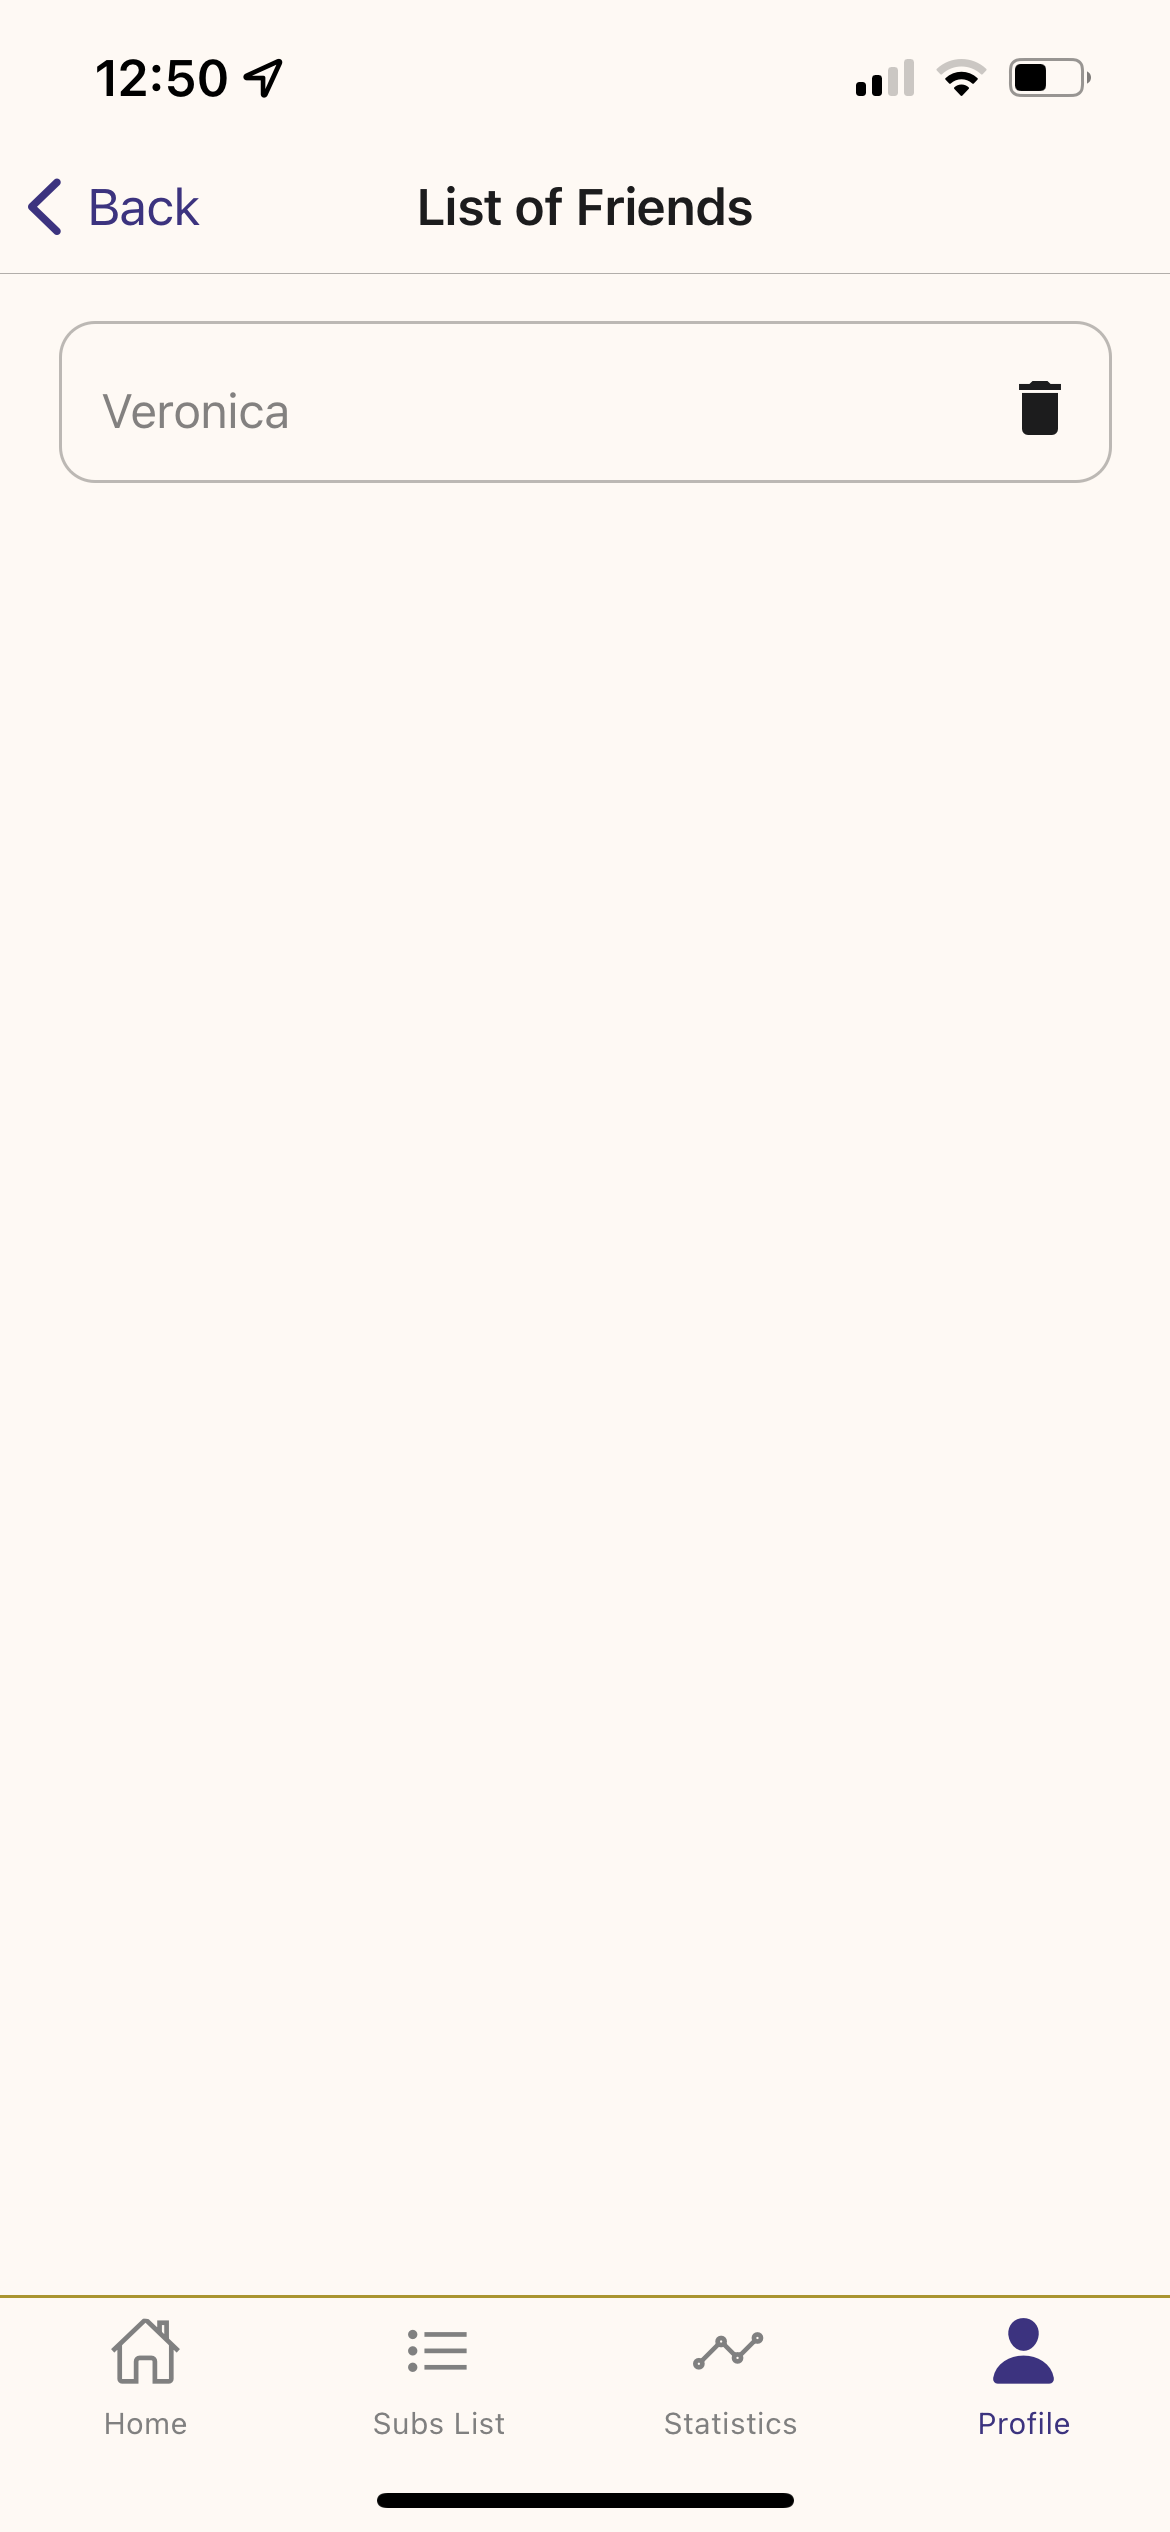
\includegraphics[width=0.6\textwidth, clip]{../../assets/smartphone/listFriends.PNG}
        \caption{List of friends: they can be deleted}
        \label{fig:listFriends}
    \end{minipage}
\end{figure}

\clearpage
\subsubsection{Tablet Application}

\begin{figure}[h!]
    \begin{center}
        \includegraphics[width=0.7\textwidth, clip]{../../assets/tablet/login.png}
    \end{center}
    \caption{Login page}
    \label{fig:tlogin}
\end{figure}

\begin{figure}[h!]
    \begin{center}
        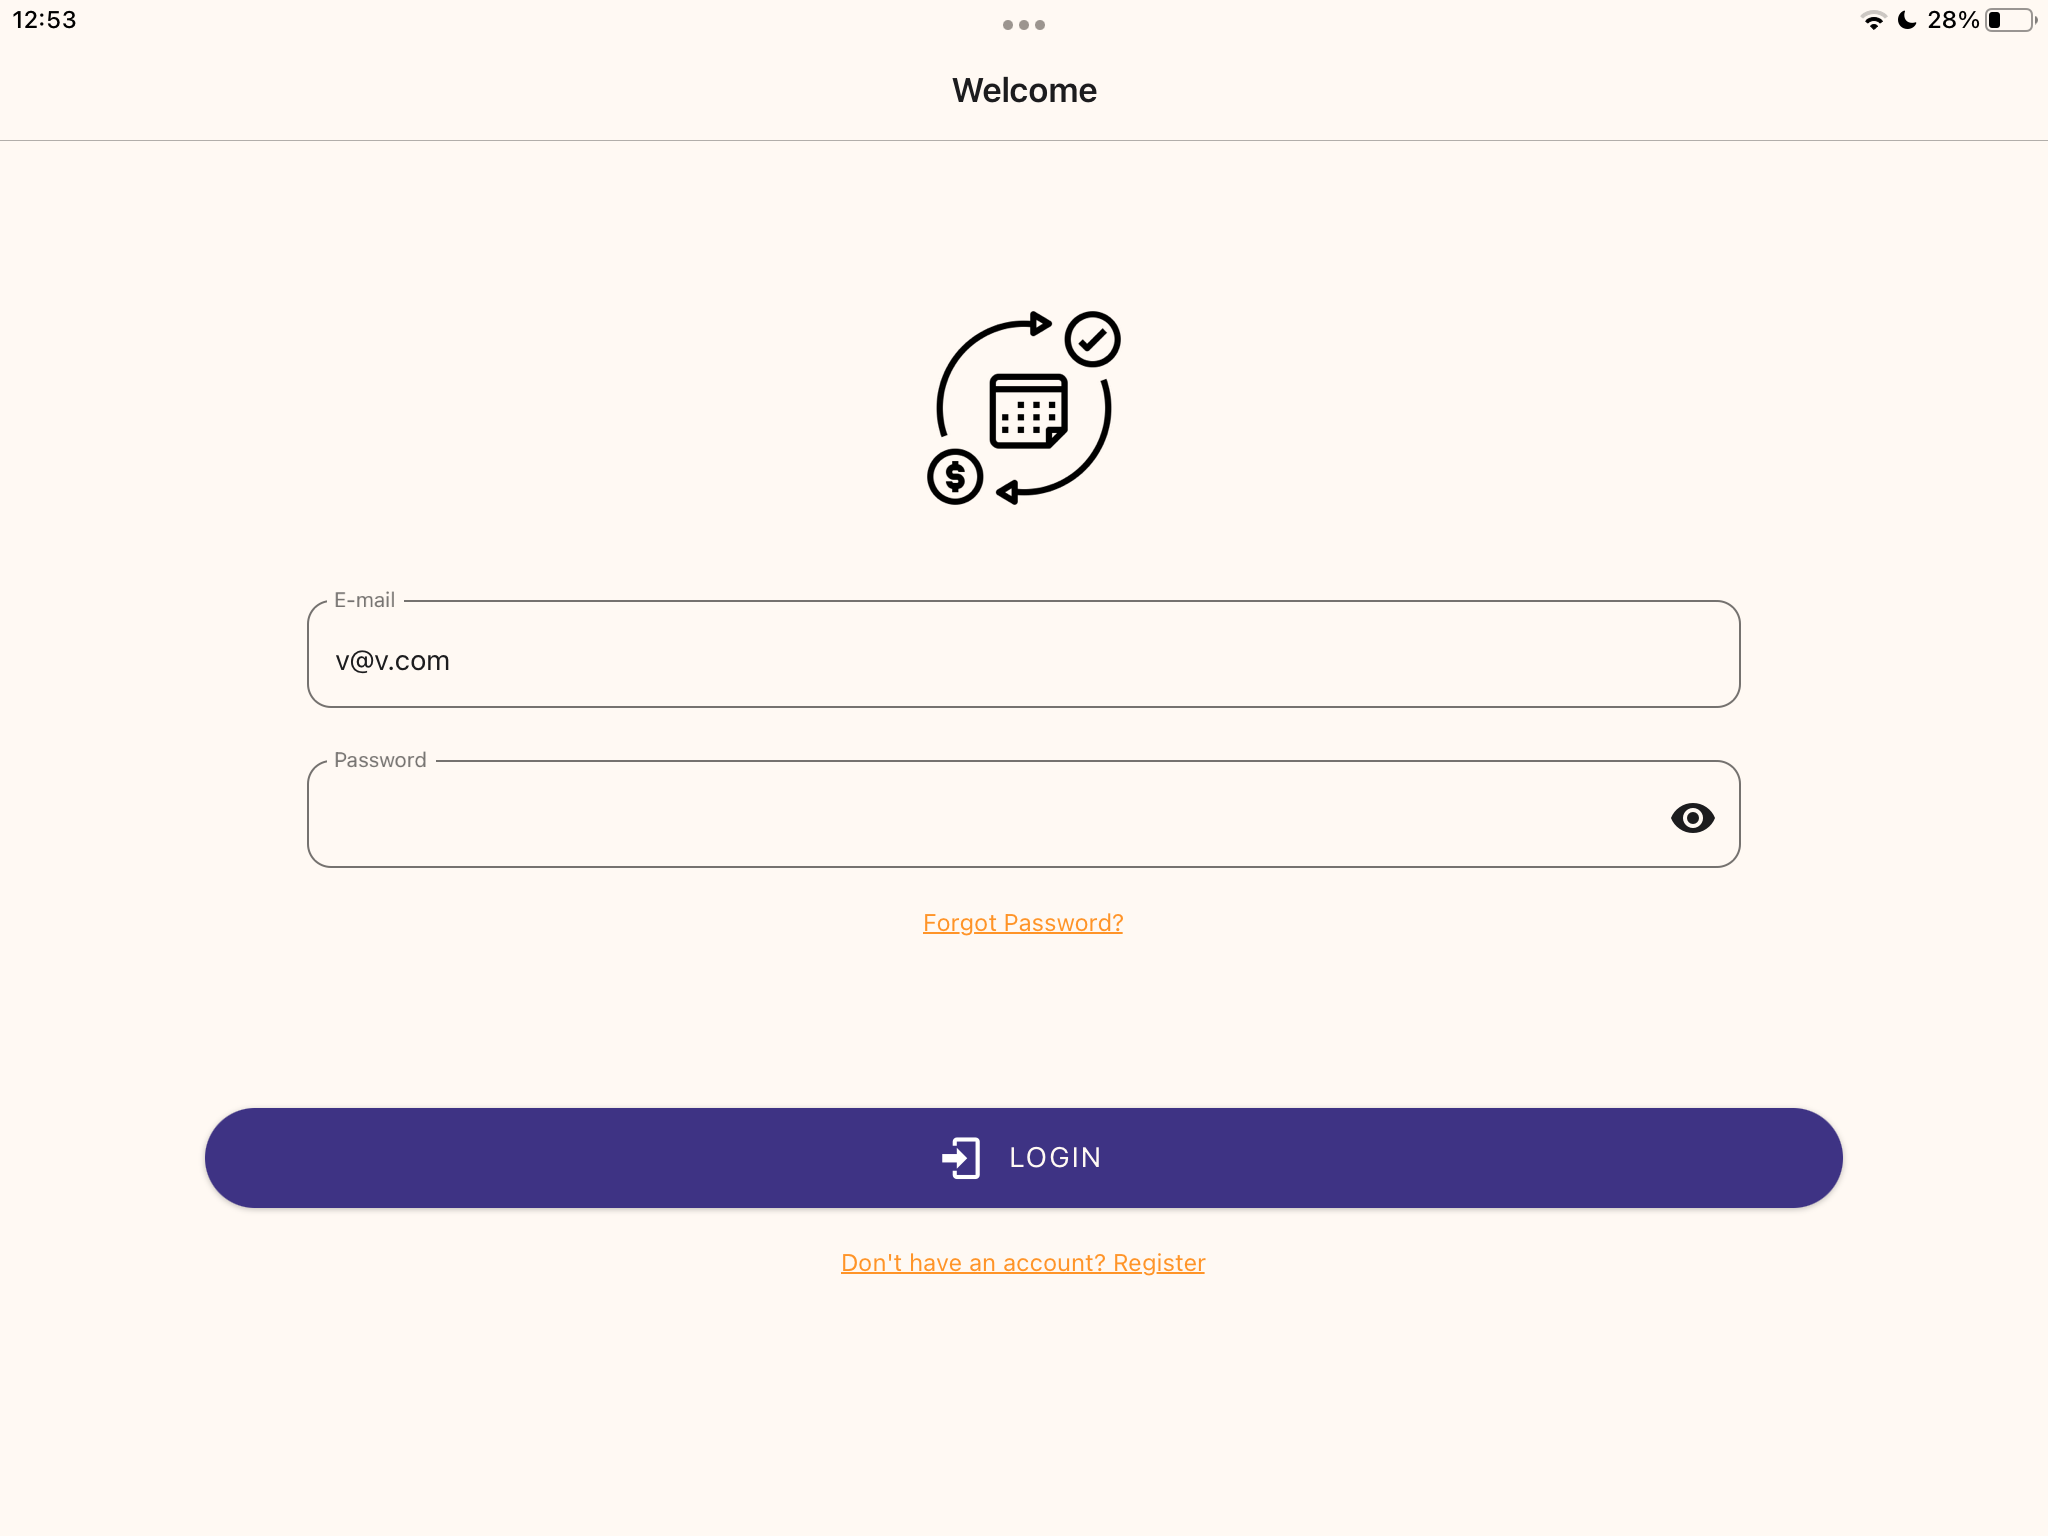
\includegraphics[width=0.7\textwidth, clip]{../../assets/tablet/loginActive.png}
    \end{center}
    \caption{Login page with button activated after insertion of fields}
    \label{fig:tloginActive}
\end{figure}

\begin{figure}[h!]
    \begin{center}
        \includegraphics[width=0.7\textwidth, clip]{../../assets/tablet/reg.png}
    \end{center}
    \caption{Registration page with strong password indicator}
    \label{fig:treg}
\end{figure}

\begin{figure}[h!]
    \begin{center}
        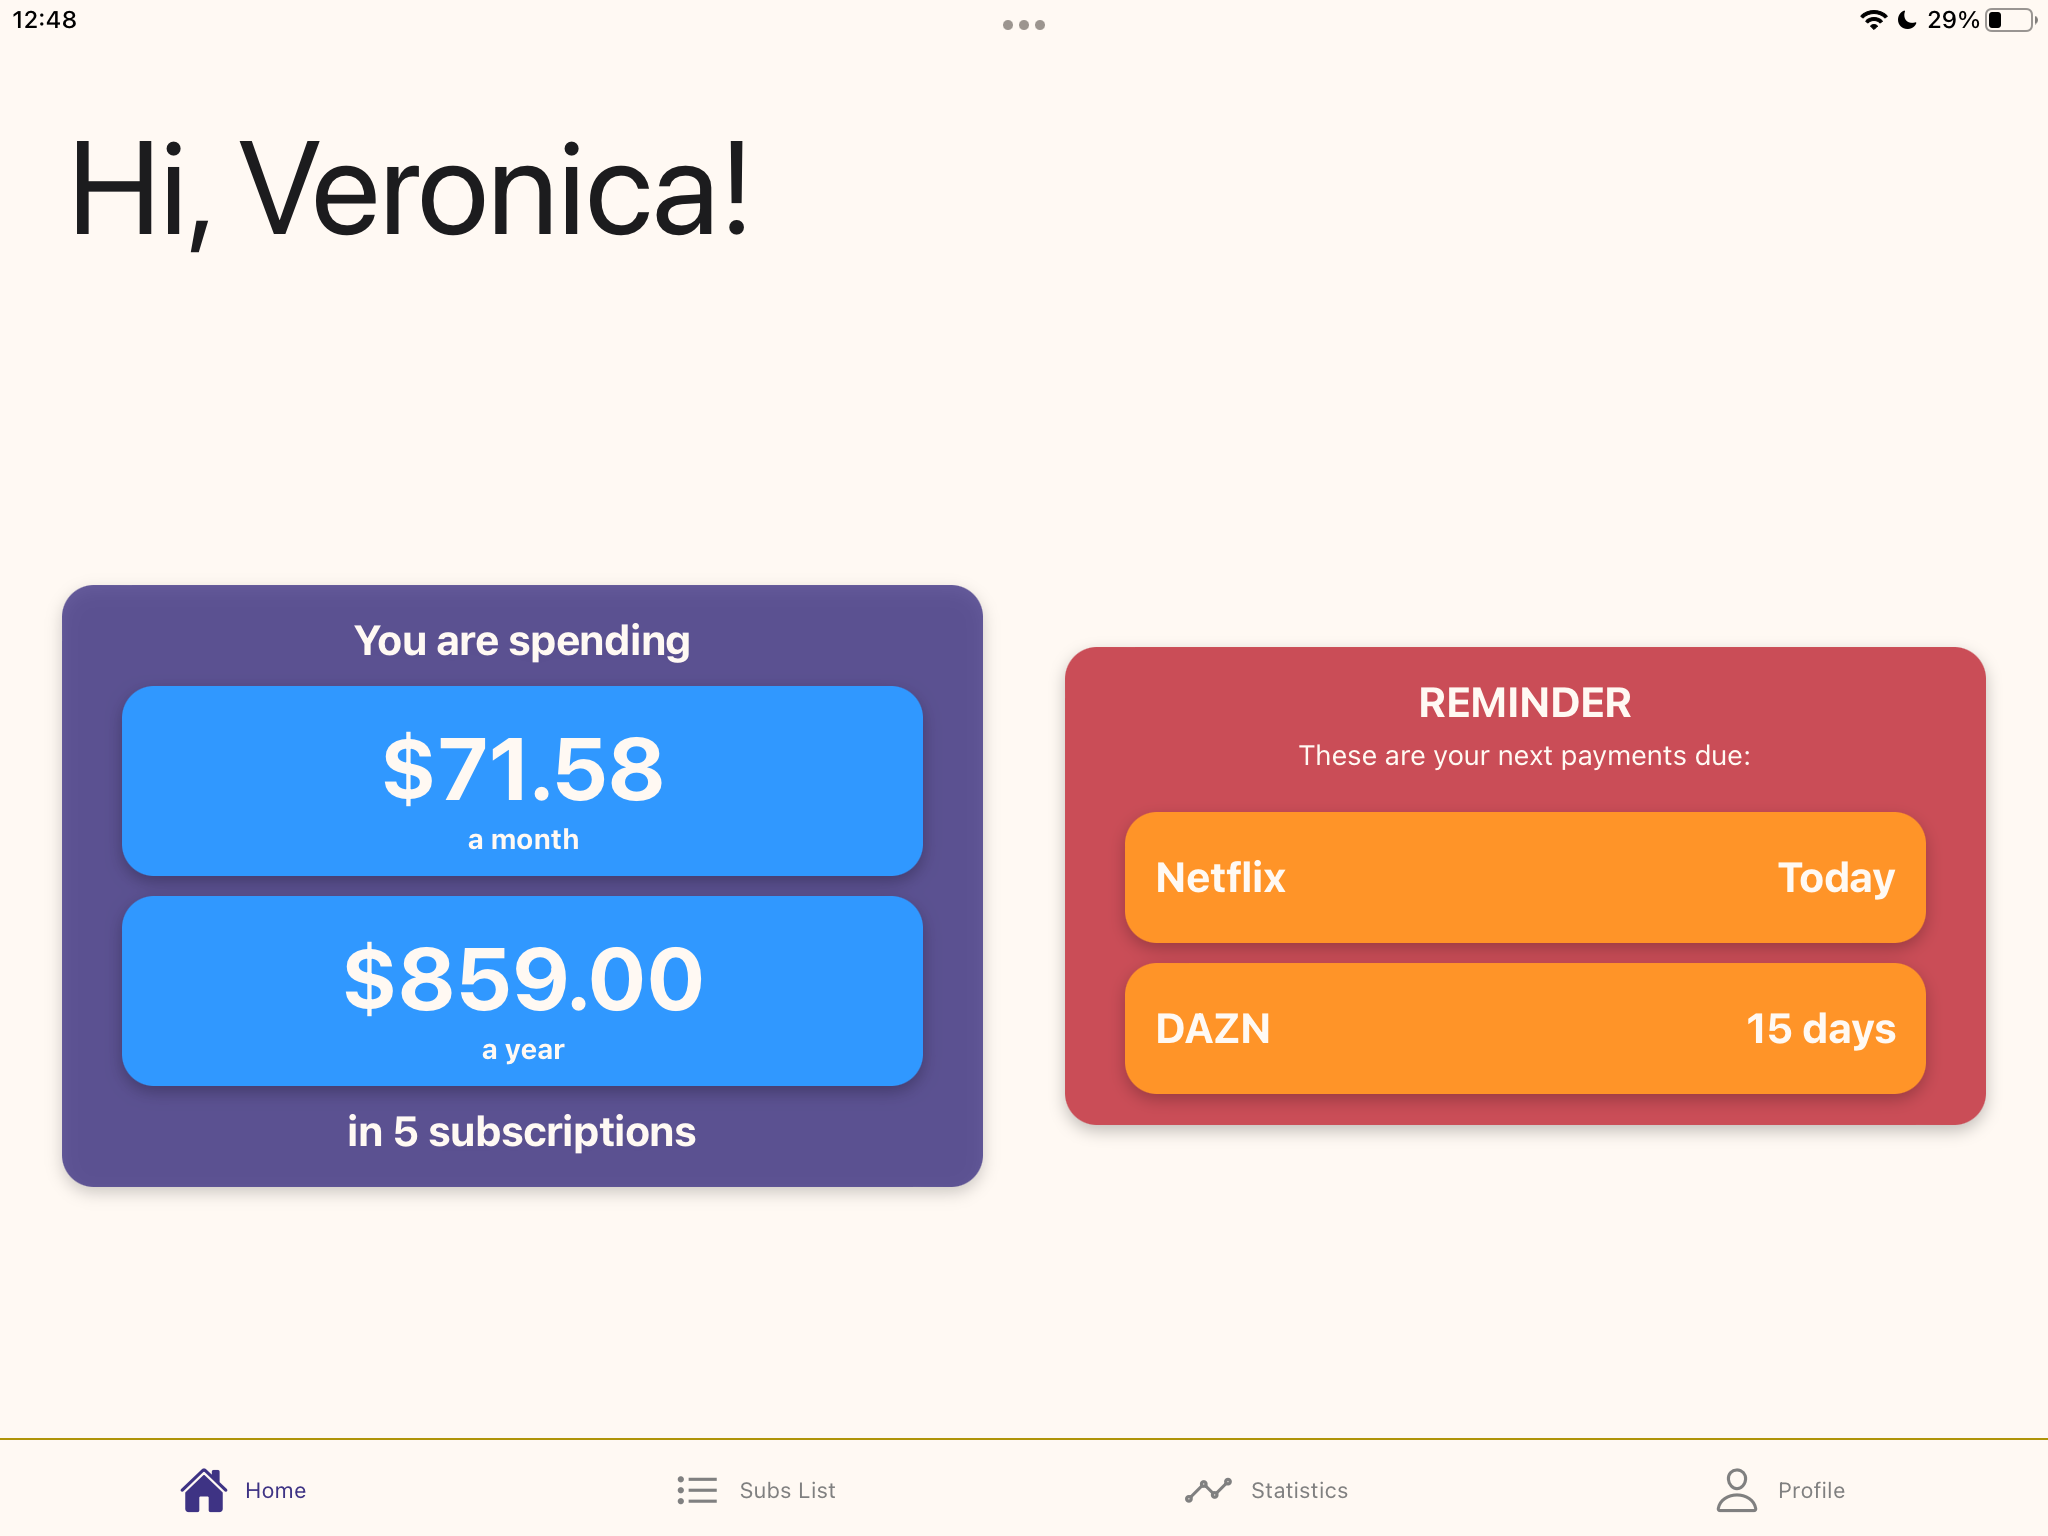
\includegraphics[width=0.7\textwidth, clip]{../../assets/tablet/home.png}
    \end{center}
    \caption{Home page, customized layout due to landscape mode and bigger screen}
    \label{fig:thome}
\end{figure}

\begin{figure}[h!]
    \begin{center}
        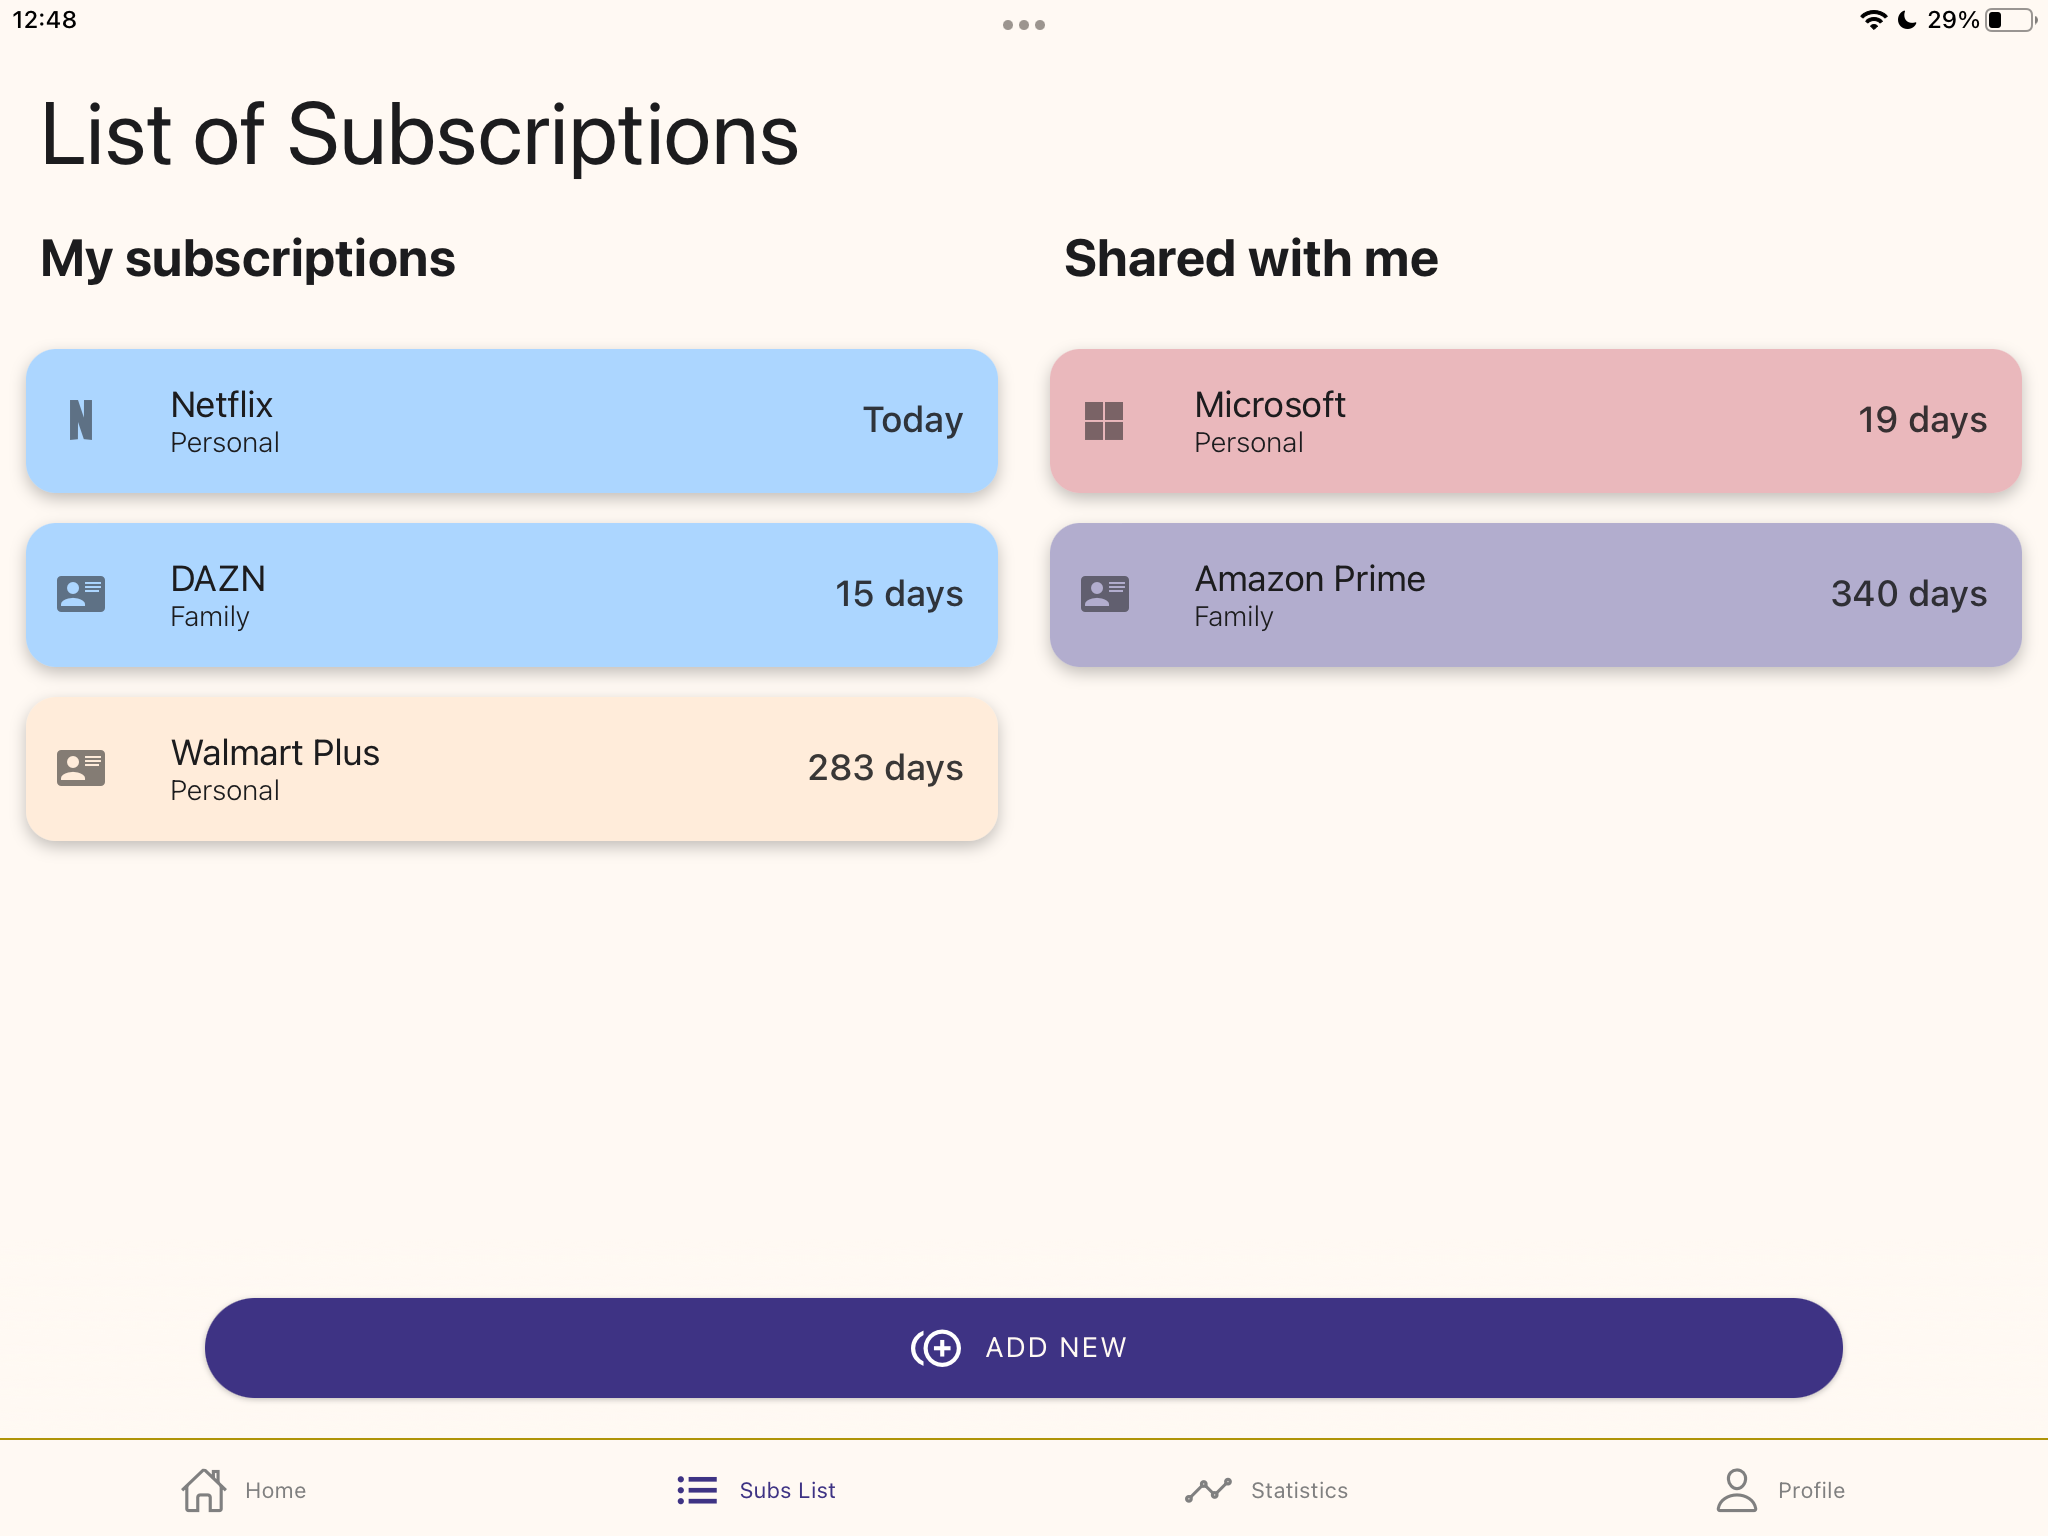
\includegraphics[width=0.7\textwidth, clip]{../../assets/tablet/subsList.PNG}
    \end{center}
    \caption{List of subscriptions, divided into two columns}
    \label{fig:tsubsList}
\end{figure}

\begin{figure}[h!]
    \begin{center}
        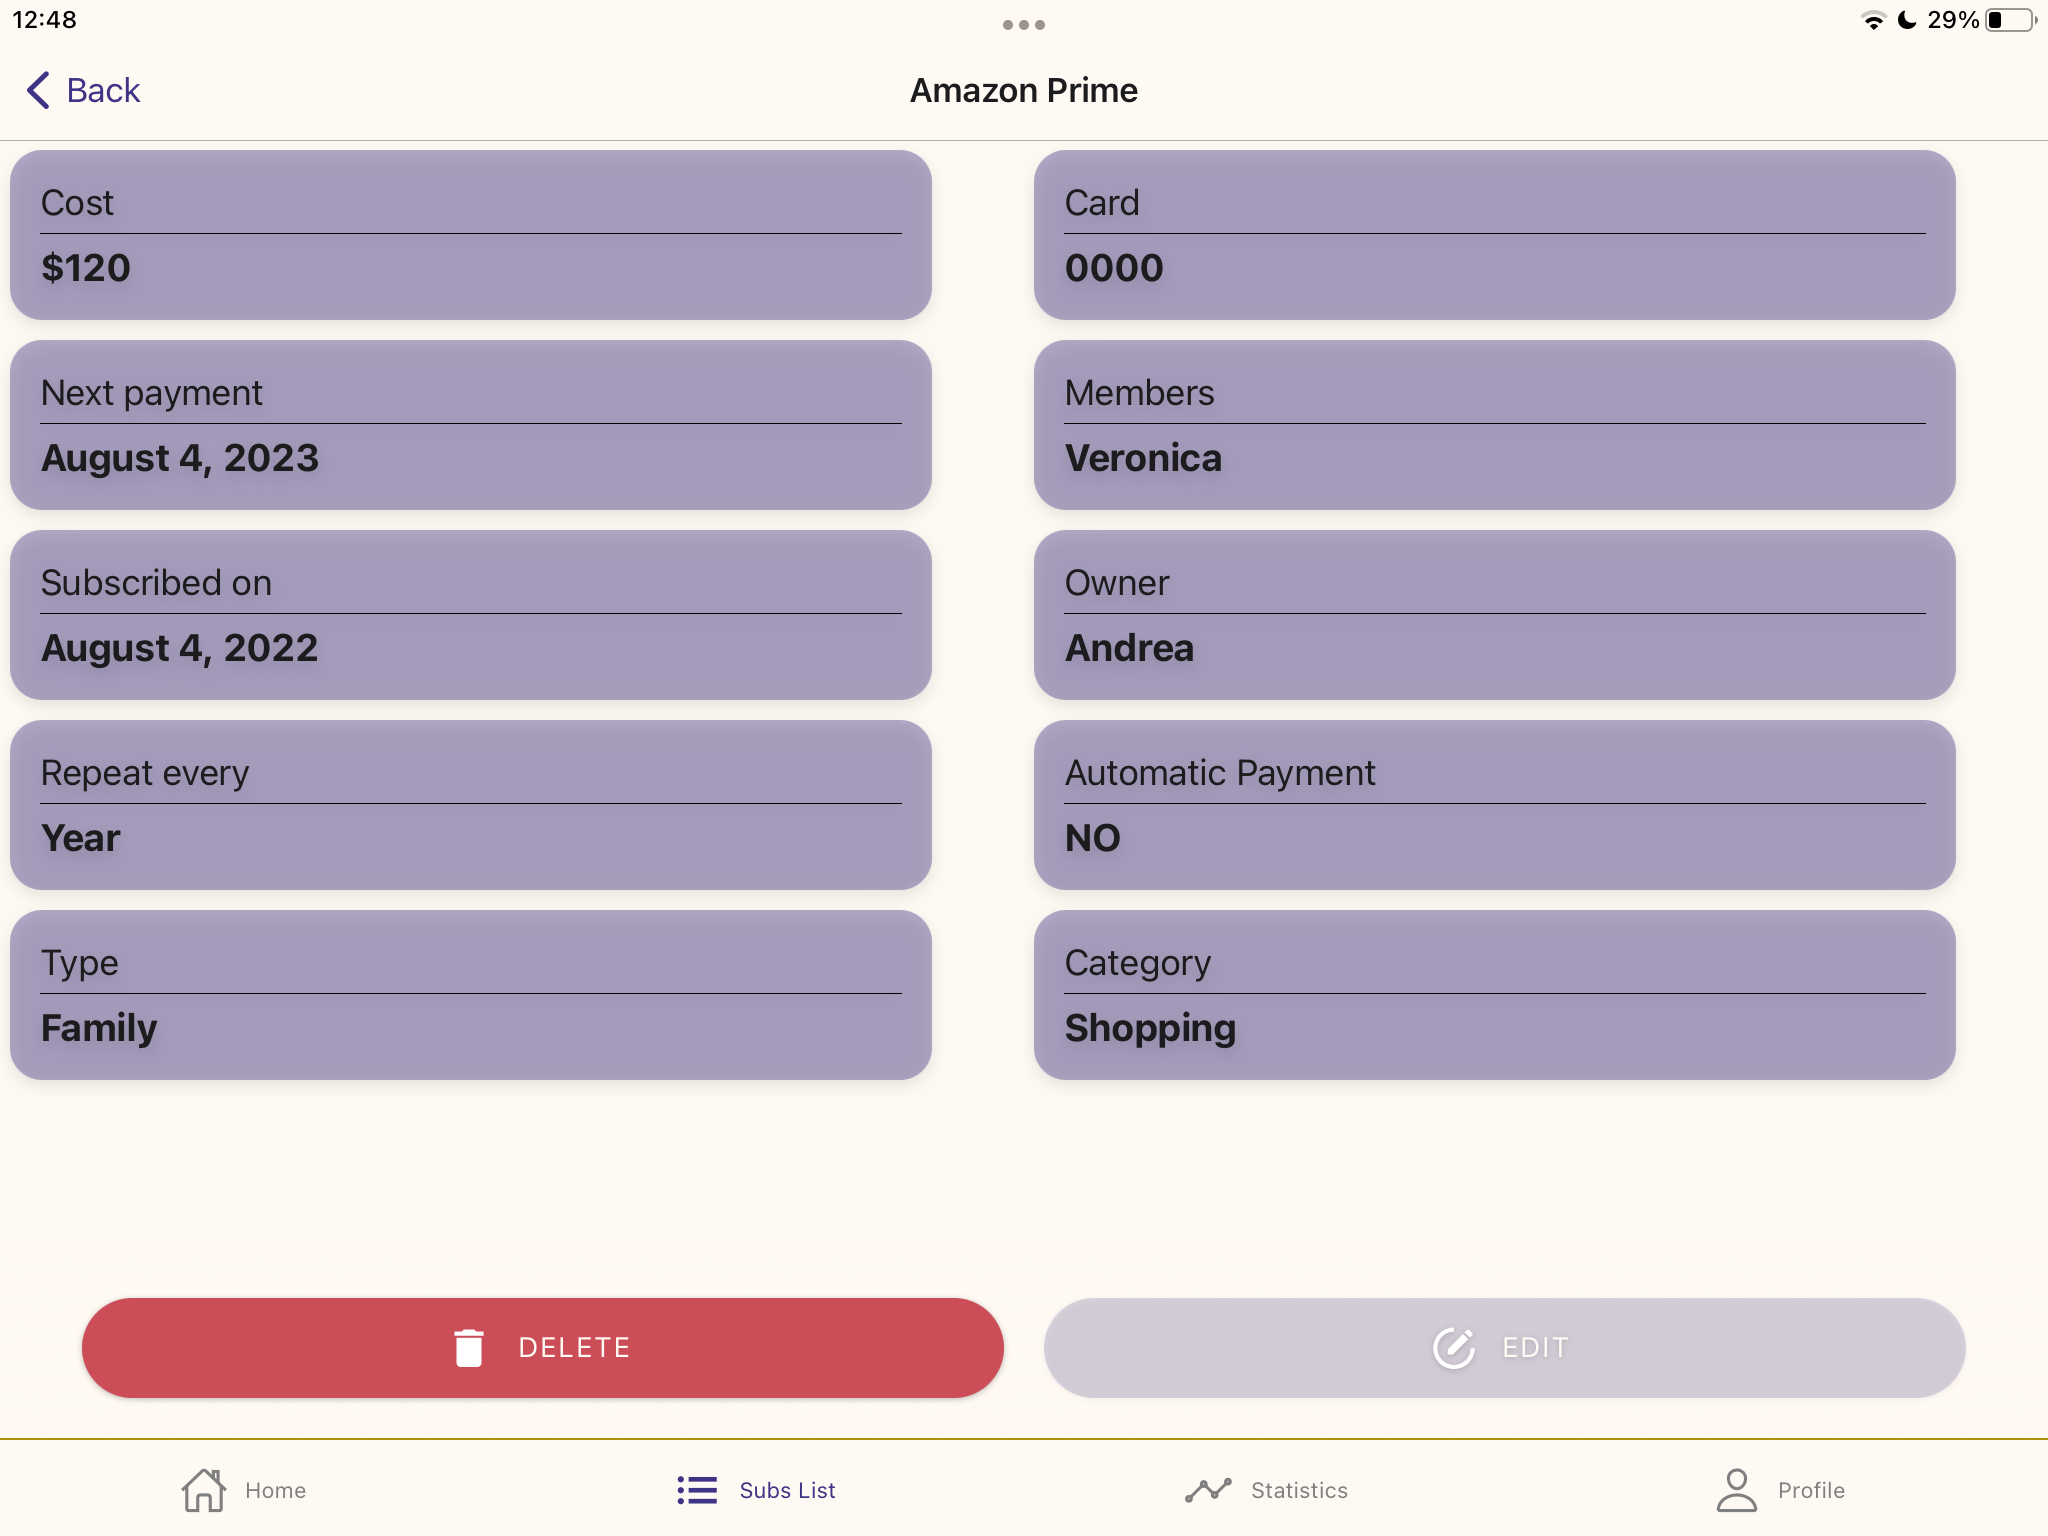
\includegraphics[width=0.7\textwidth, clip]{../../assets/tablet/detail.PNG}
    \end{center}
    \caption{Detail page: edit button disabled since the owner is `Andrea'}
    \label{fig:tdetail}
\end{figure}

\begin{figure}[h!]
    \begin{center}
        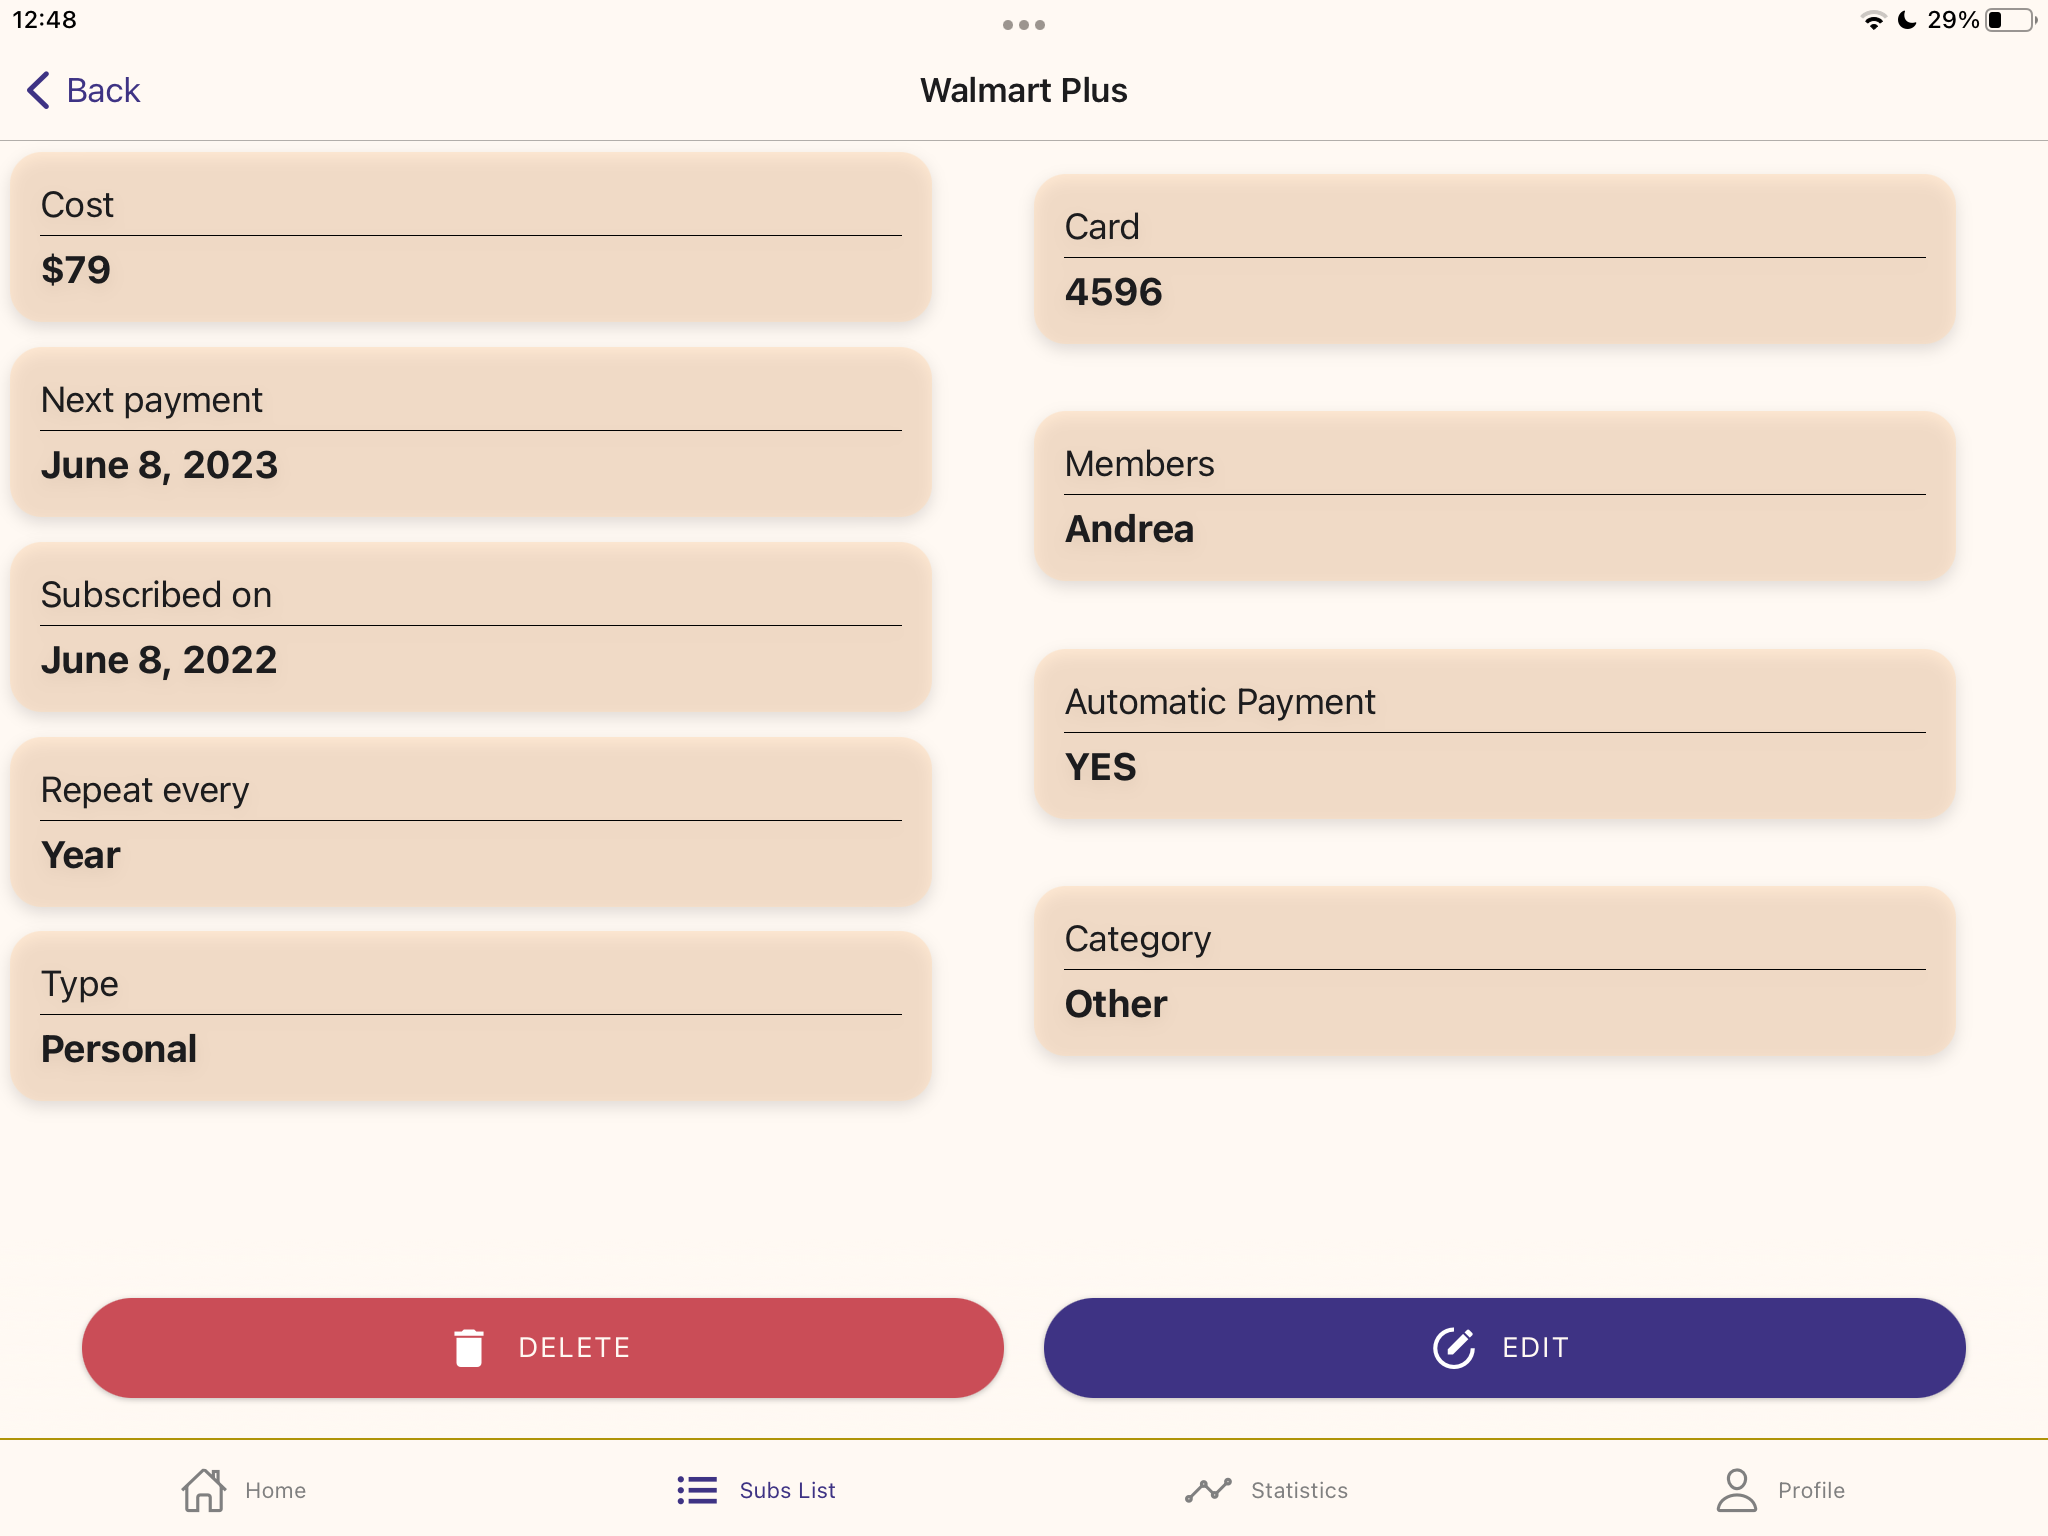
\includegraphics[width=0.7\textwidth, clip]{../../assets/tablet/detailEd.PNG}
    \end{center}
    \caption{Detail page: edit button enabled, user is owner}
    \label{fig:detailEd}
\end{figure}

\begin{figure}[h!]
    \begin{center}
        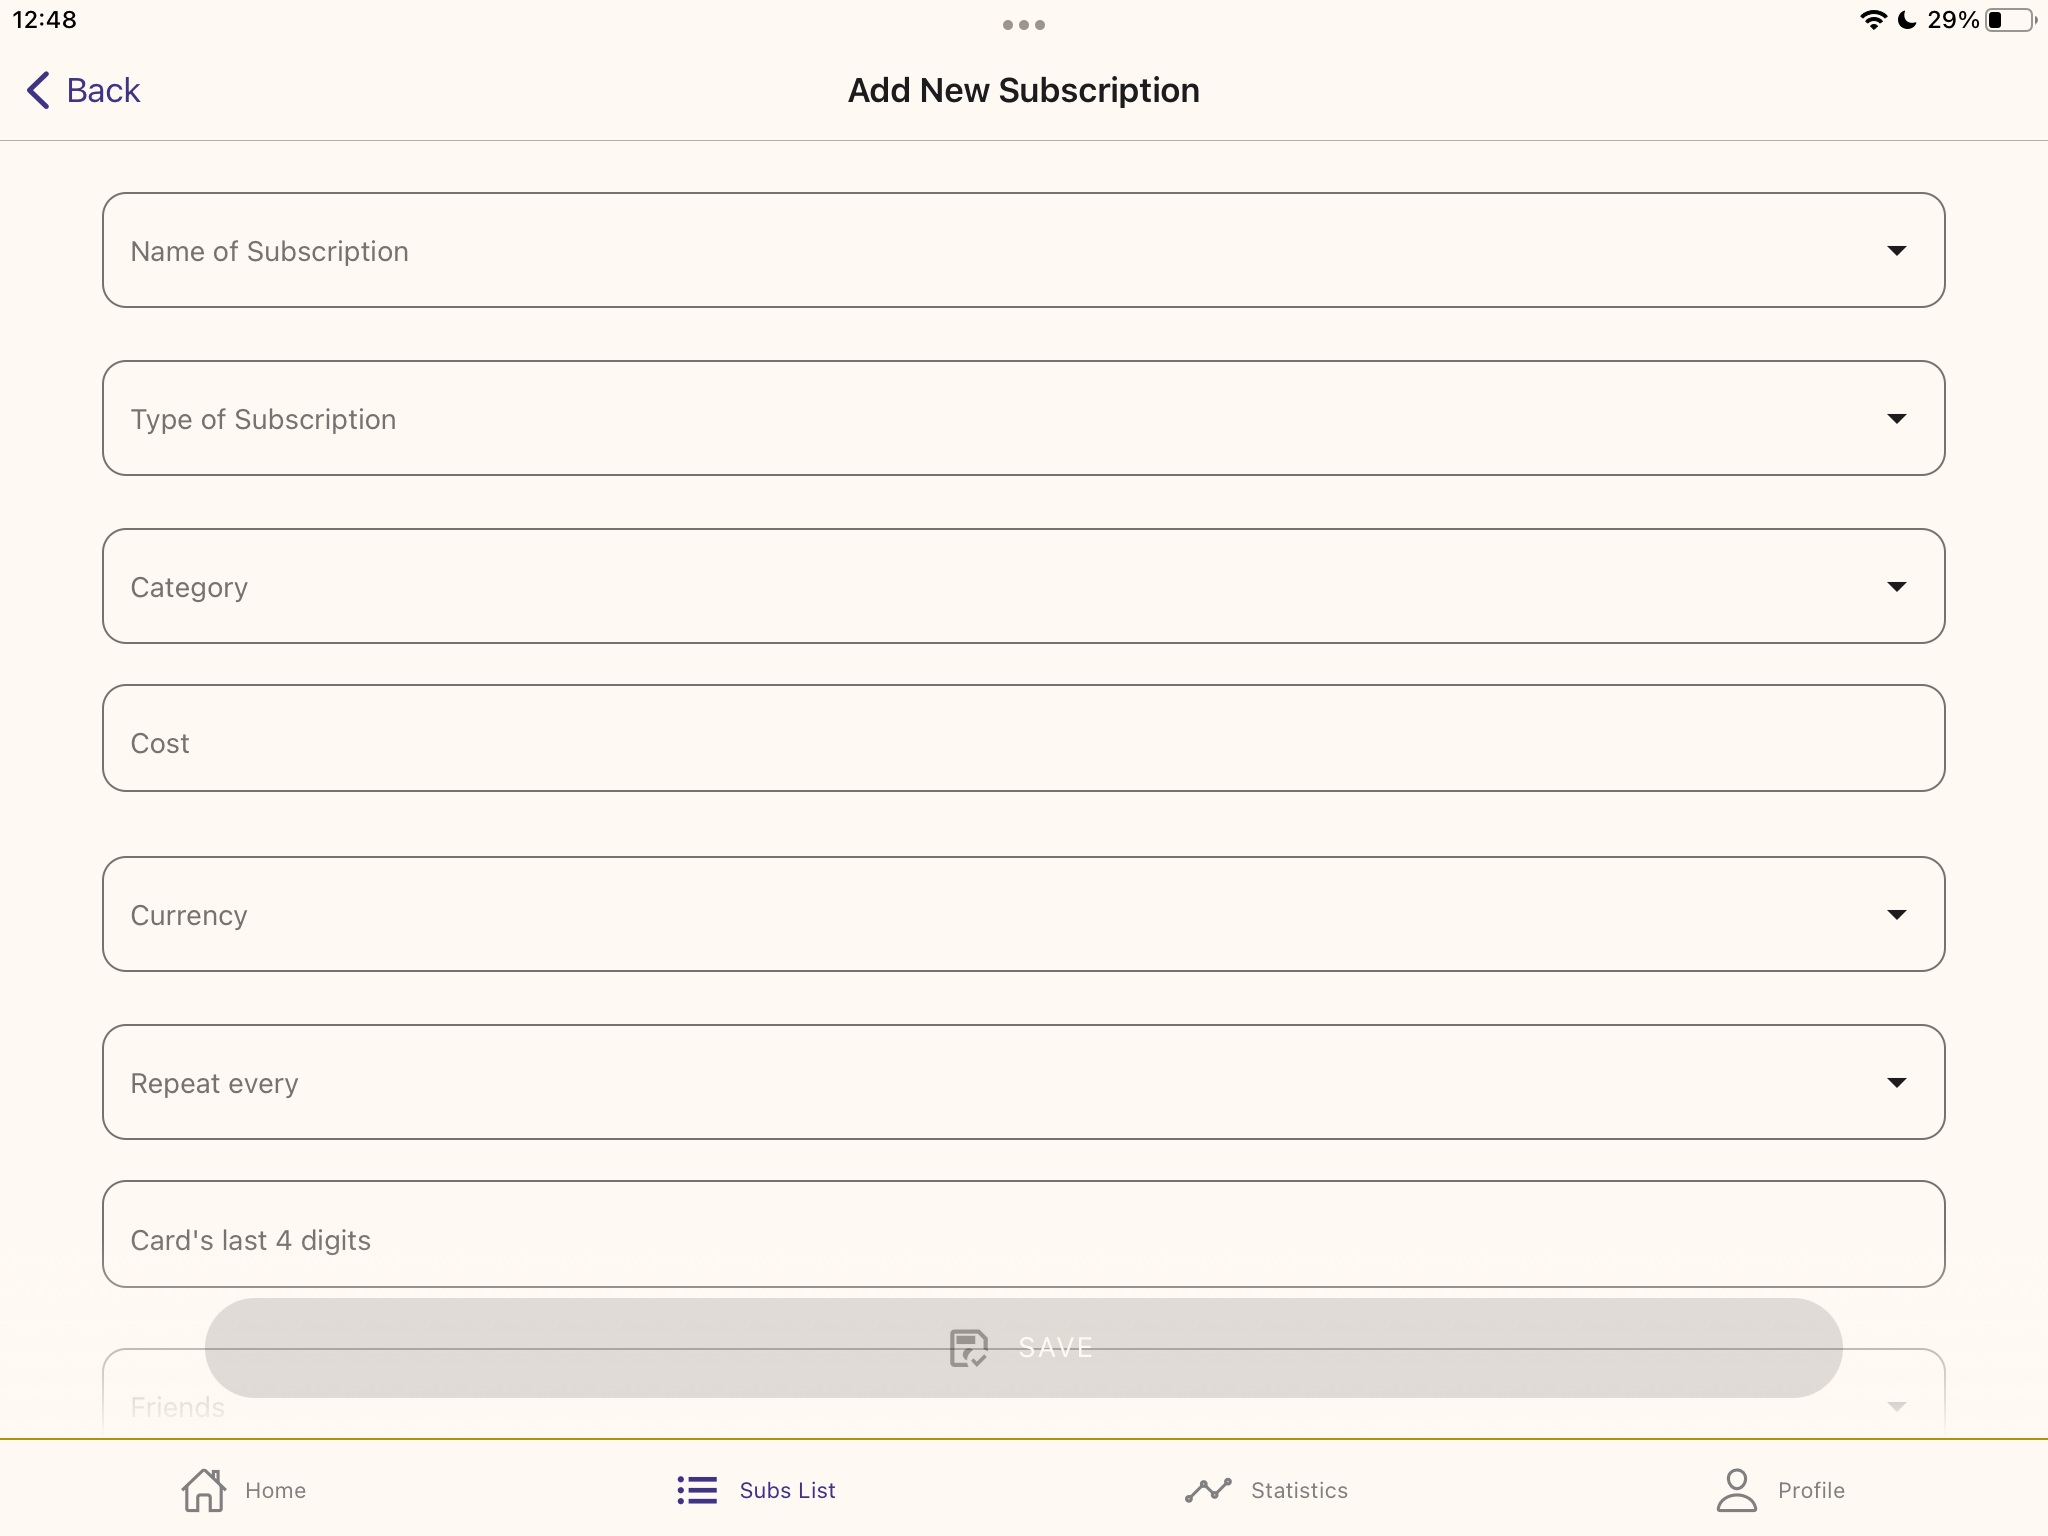
\includegraphics[width=0.7\textwidth, clip]{../../assets/tablet/add.PNG}
    \end{center}
    \caption{Add form}
    \label{fig:tadd}
\end{figure}

\begin{figure}[h!]
    \begin{center}
        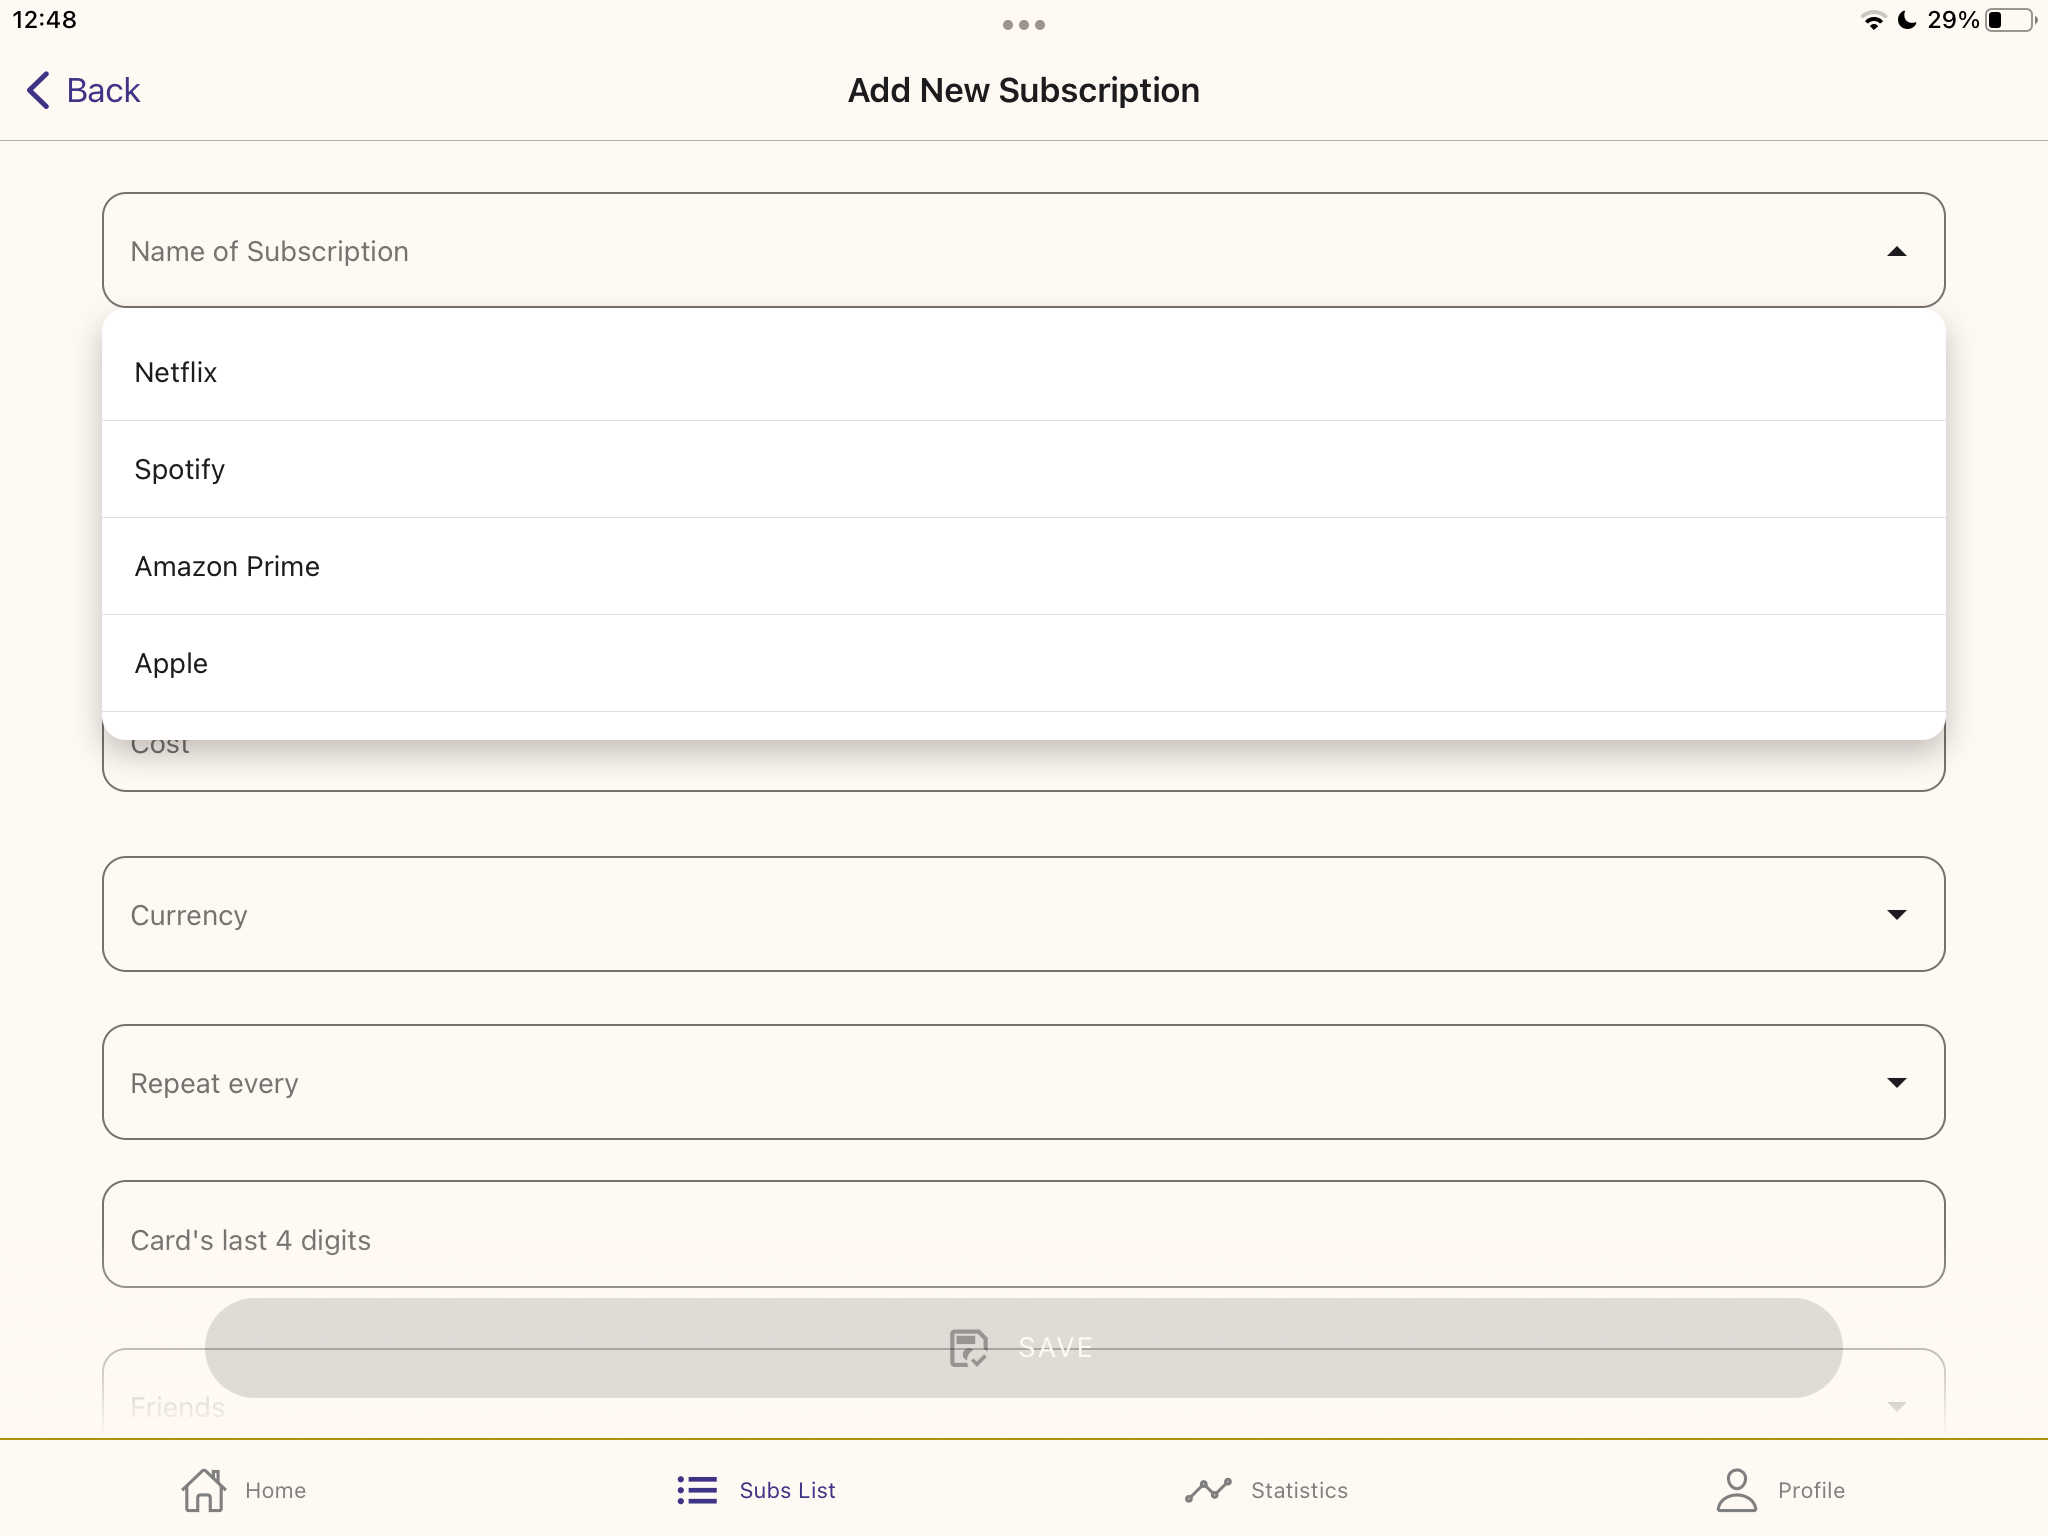
\includegraphics[width=0.7\textwidth, clip]{../../assets/tablet/addDrop.PNG}
    \end{center}
    \caption{Add form: drop-down menu}
    \label{fig:taddDrop}
\end{figure}

\begin{figure}[h!]
    \begin{center}
        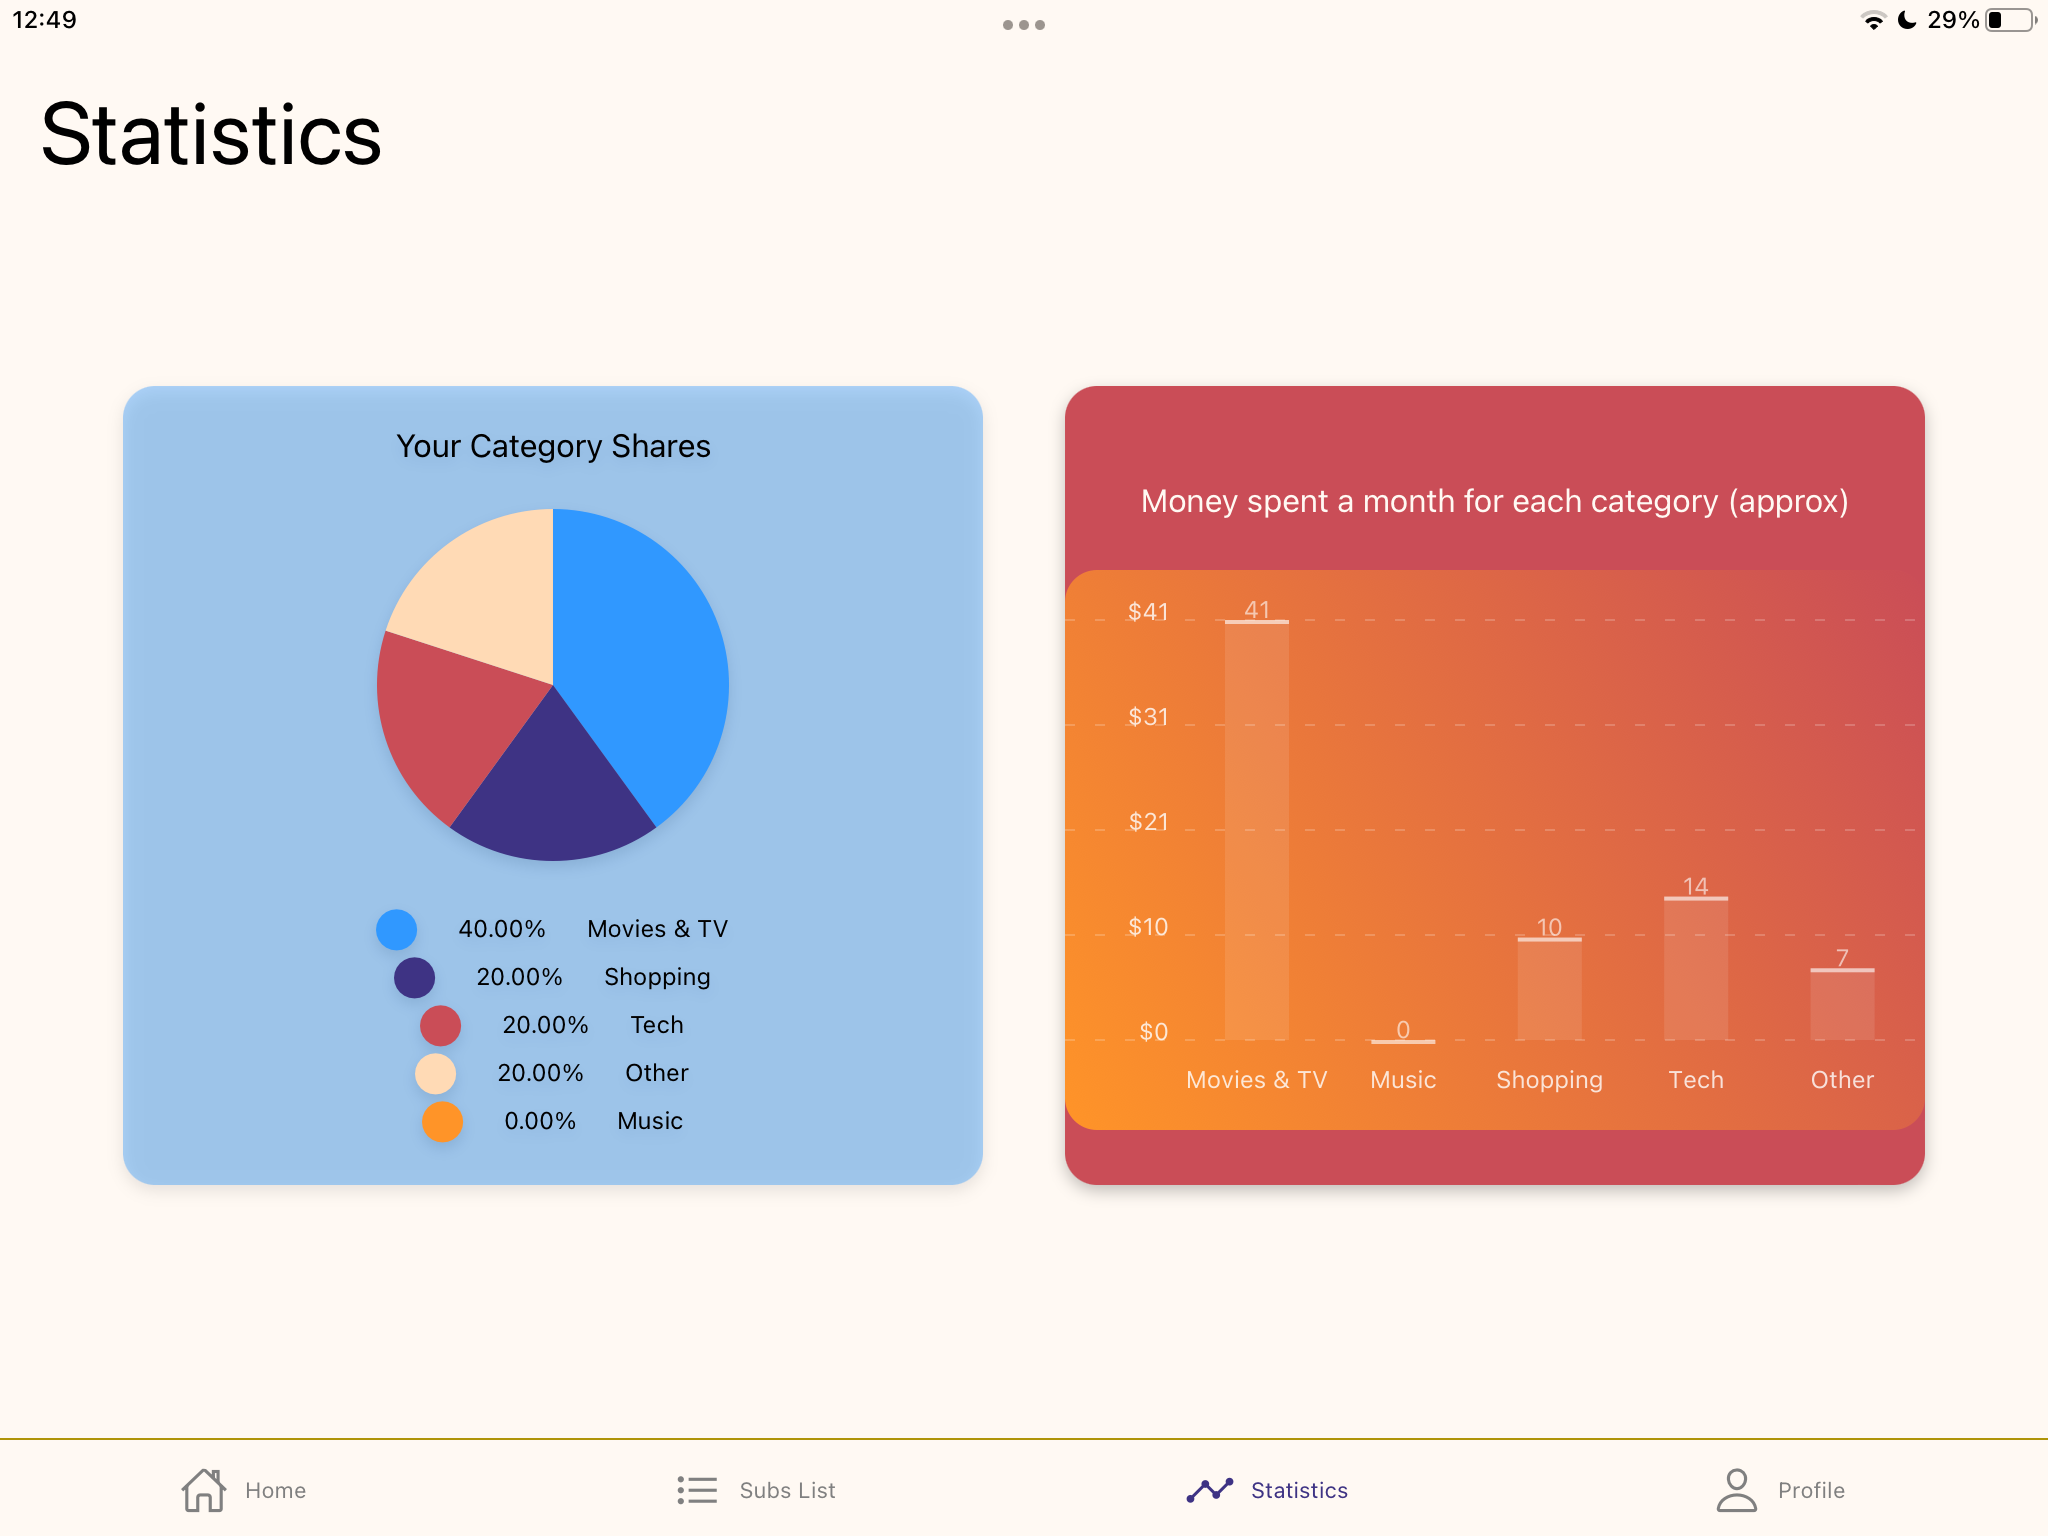
\includegraphics[width=0.7\textwidth, clip]{../../assets/tablet/stats.PNG}
    \end{center}
    \caption{Statistics: side-by-side graphs}
    \label{fig:tstats}
\end{figure}

\begin{figure}[h!]
    \begin{center}
        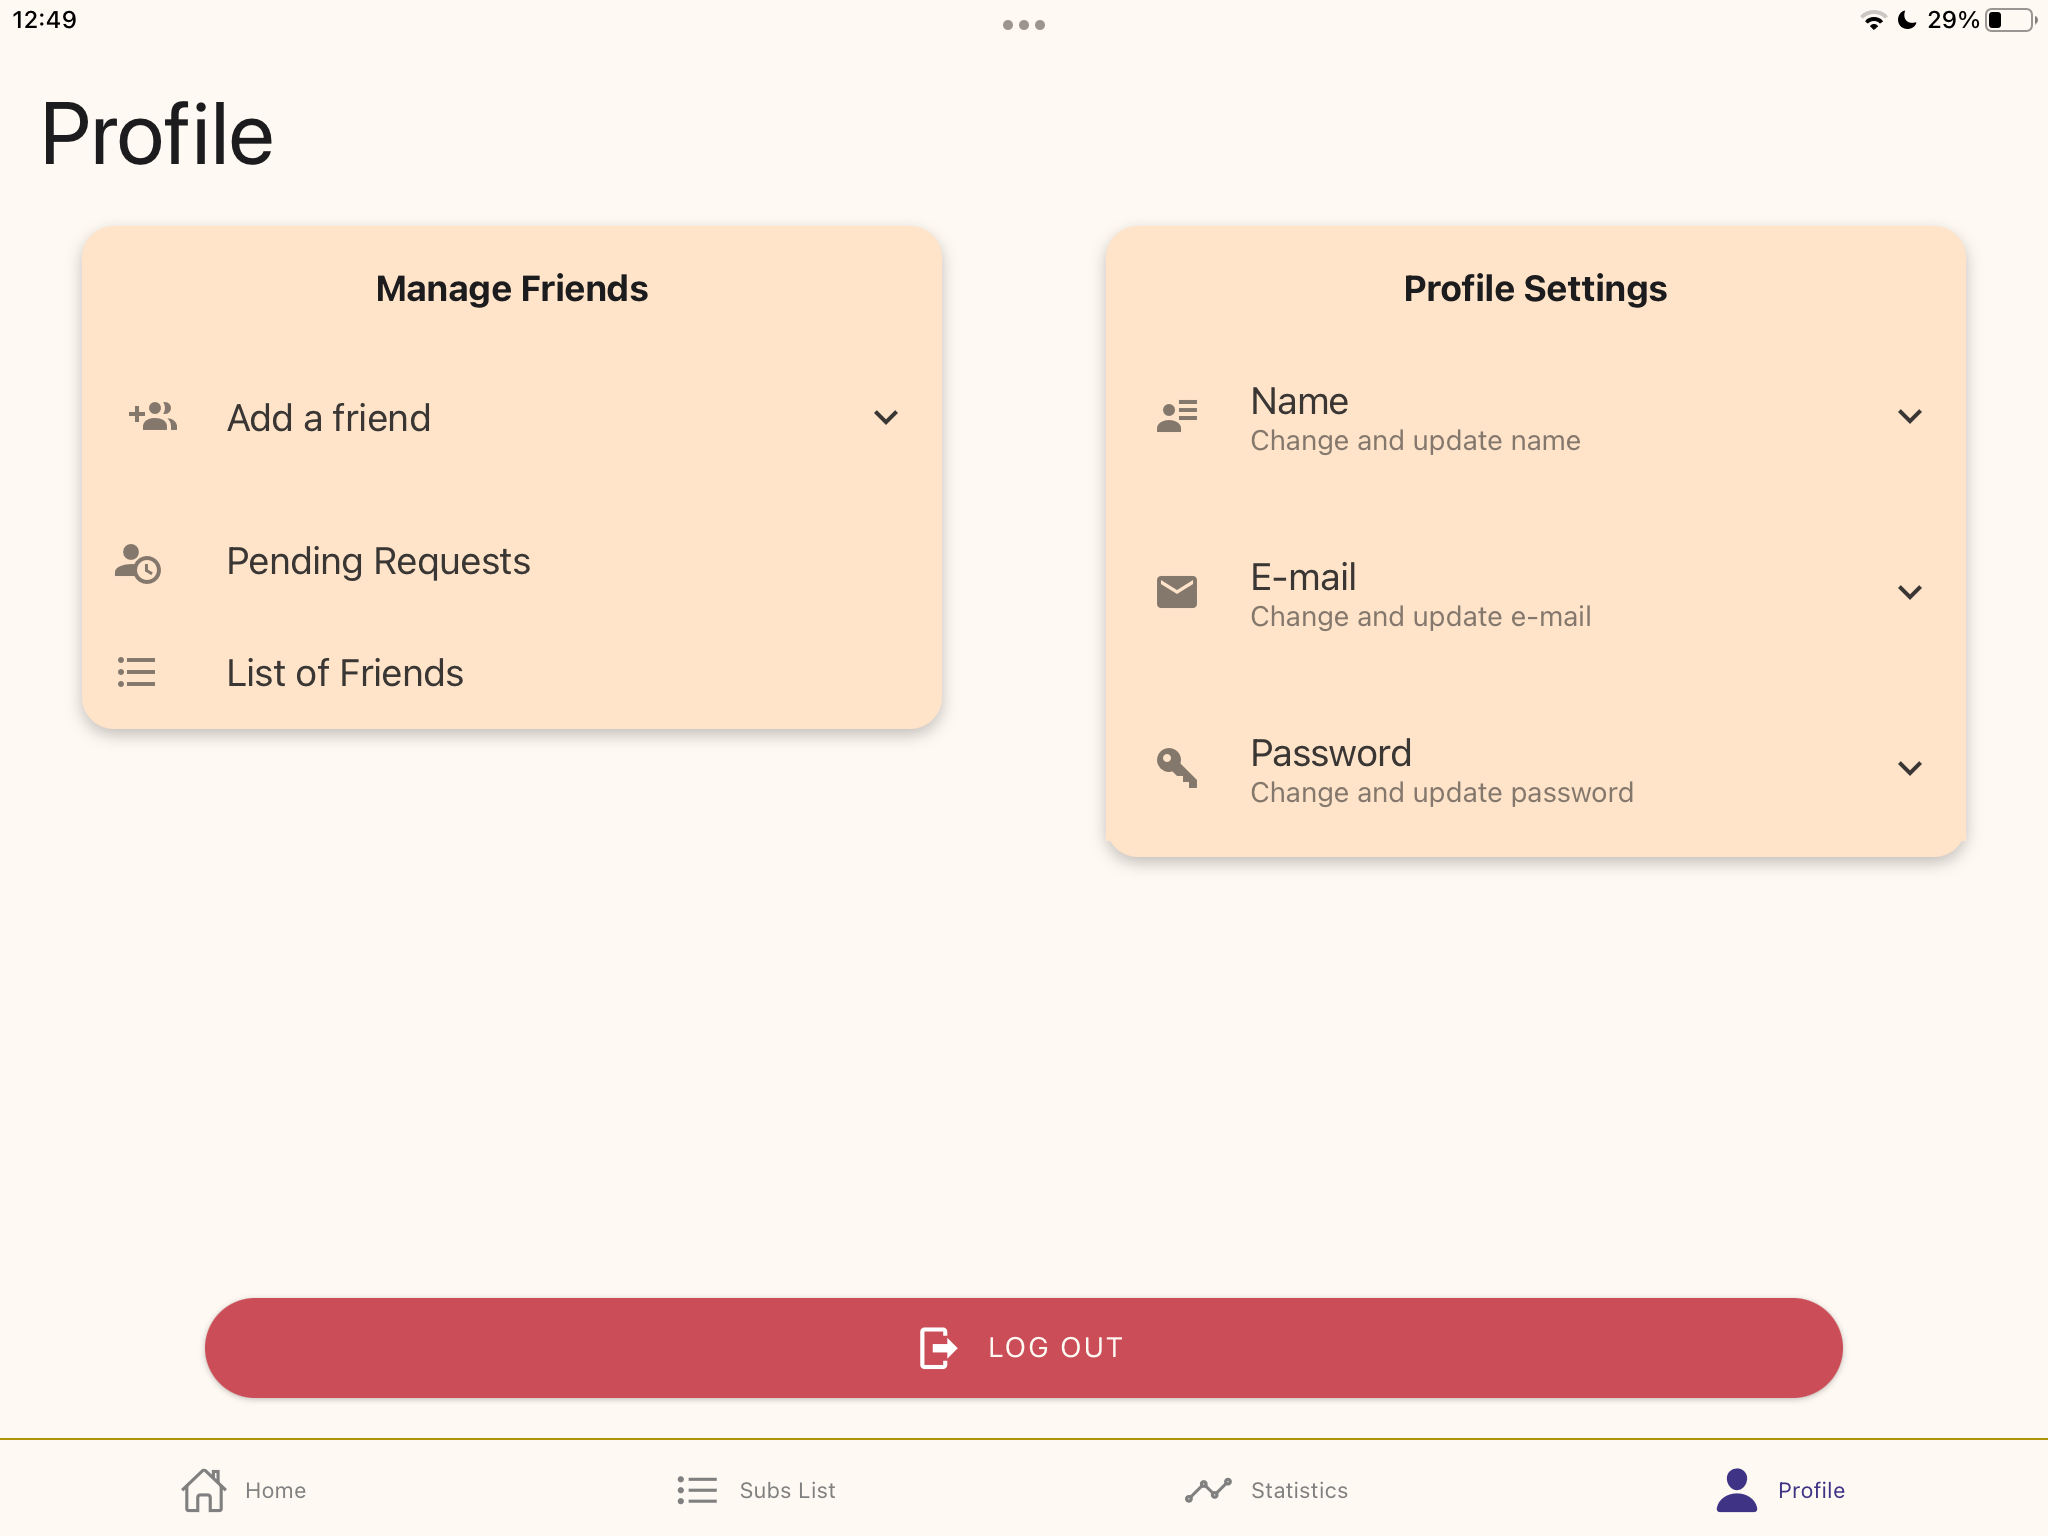
\includegraphics[width=0.7\textwidth, clip]{../../assets/tablet/profile.PNG}
    \end{center}
    \caption{Profile: side-by-side components}
    \label{fig:tprofile}
\end{figure}

\begin{figure}[h!]
    \begin{center}
        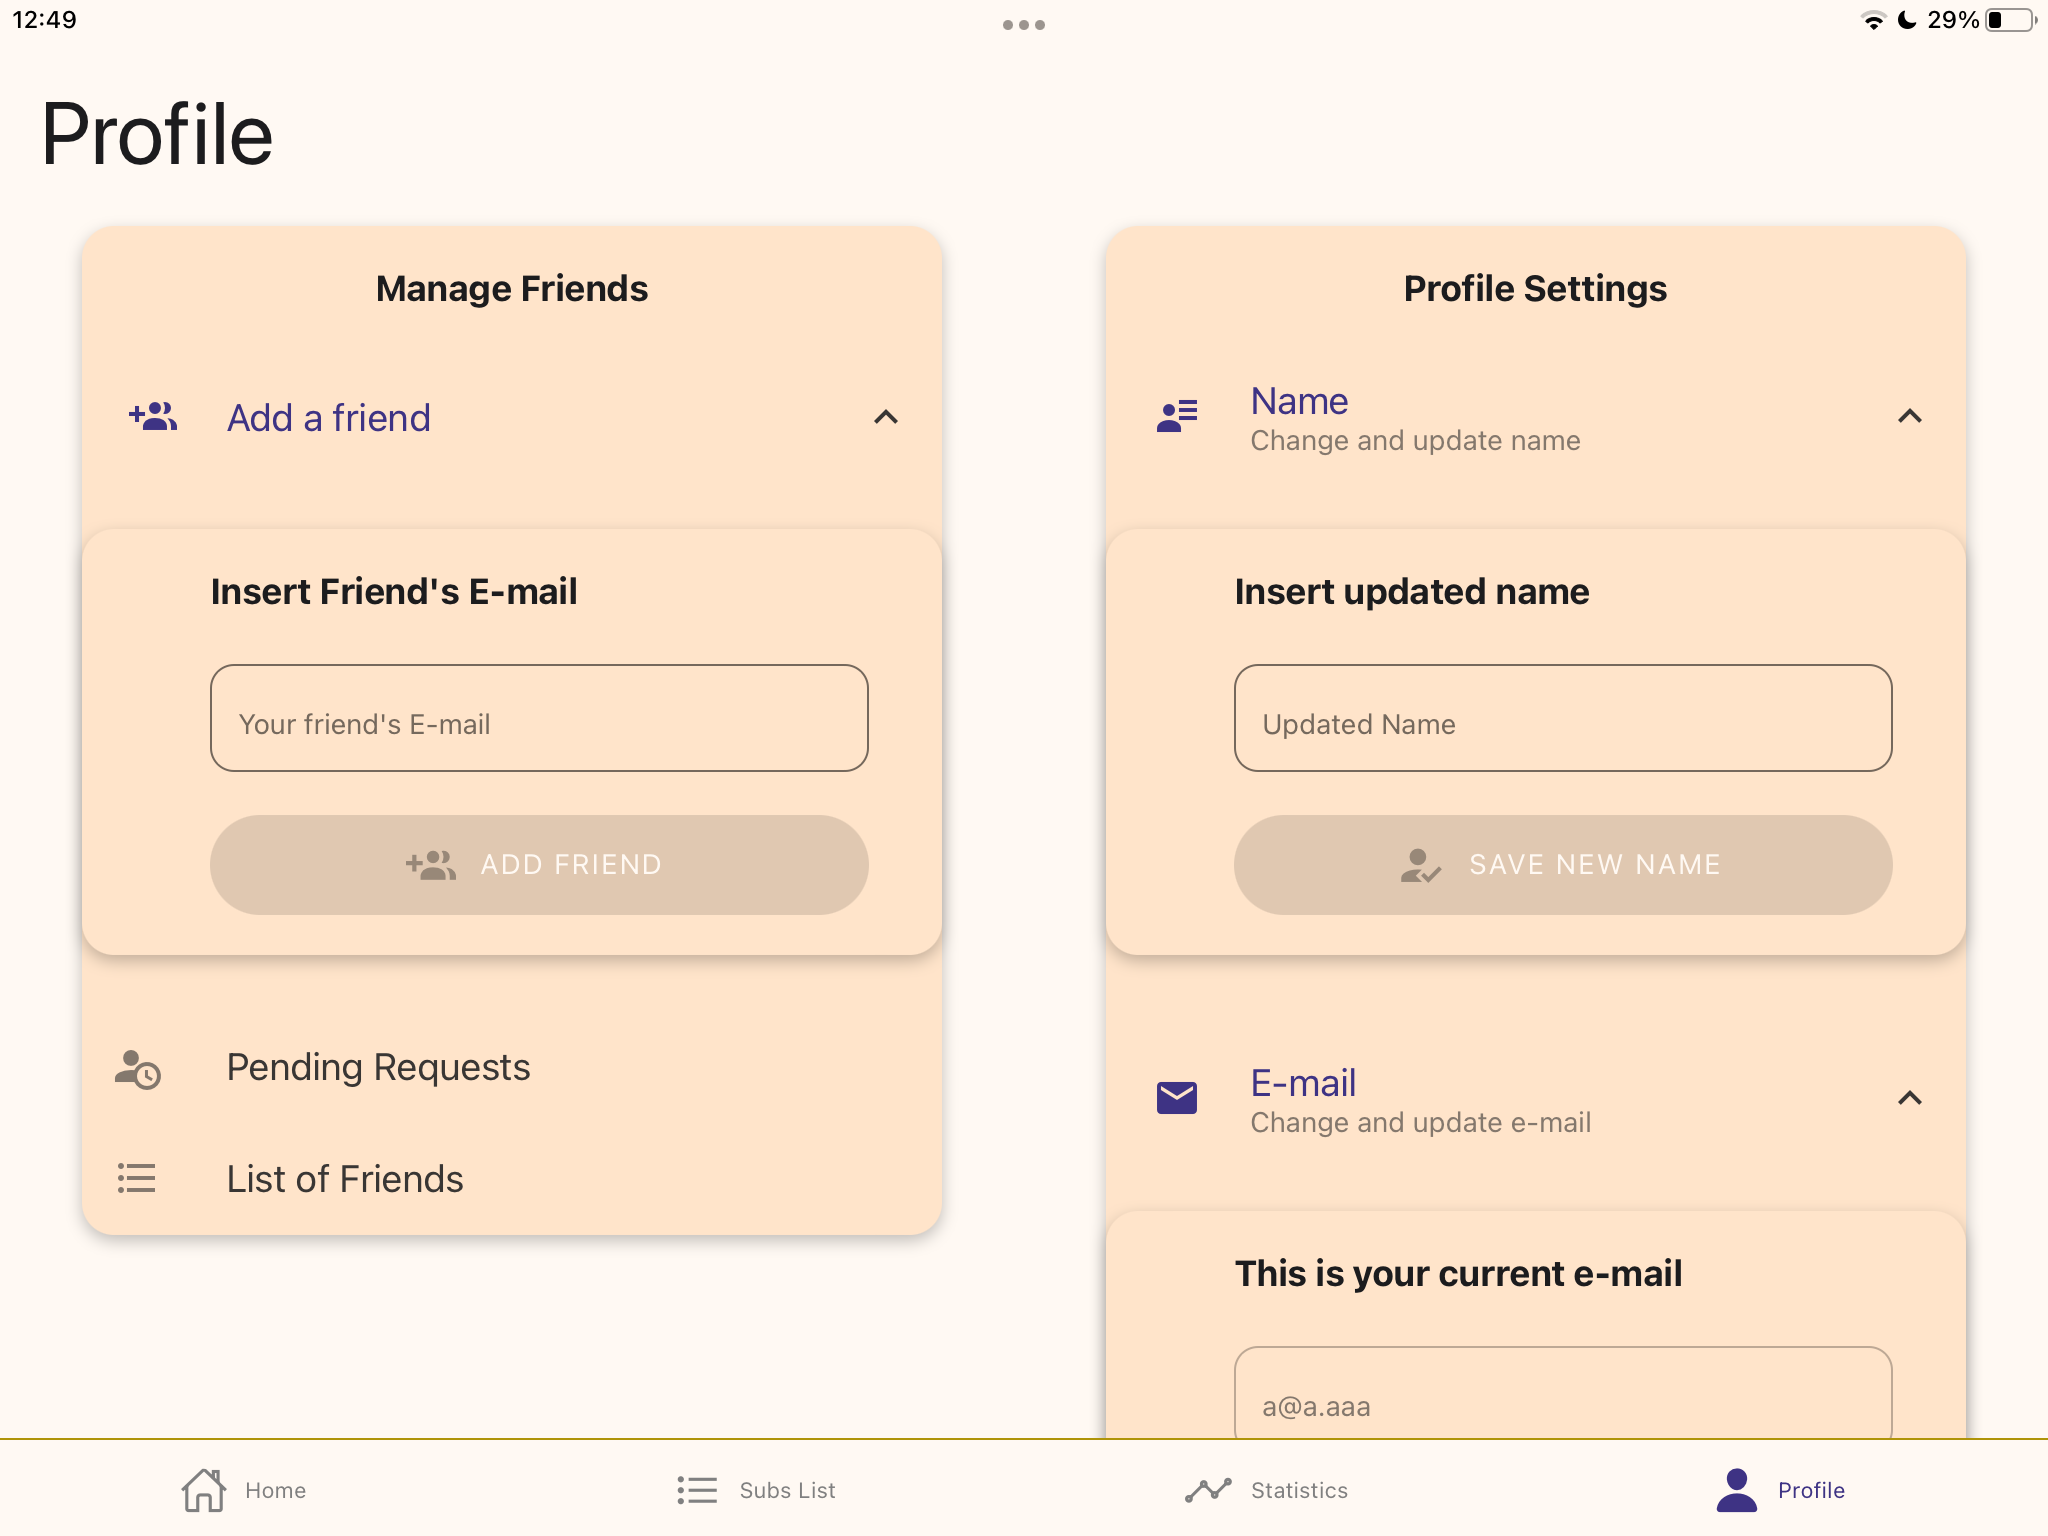
\includegraphics[width=0.7\textwidth, clip]{../../assets/tablet/profileOpen.PNG}
    \end{center}
    \caption{Profile: customizable fields shown}
    \label{fig:tprofileOpen}
\end{figure}

\begin{figure}[h!]
    \begin{center}
        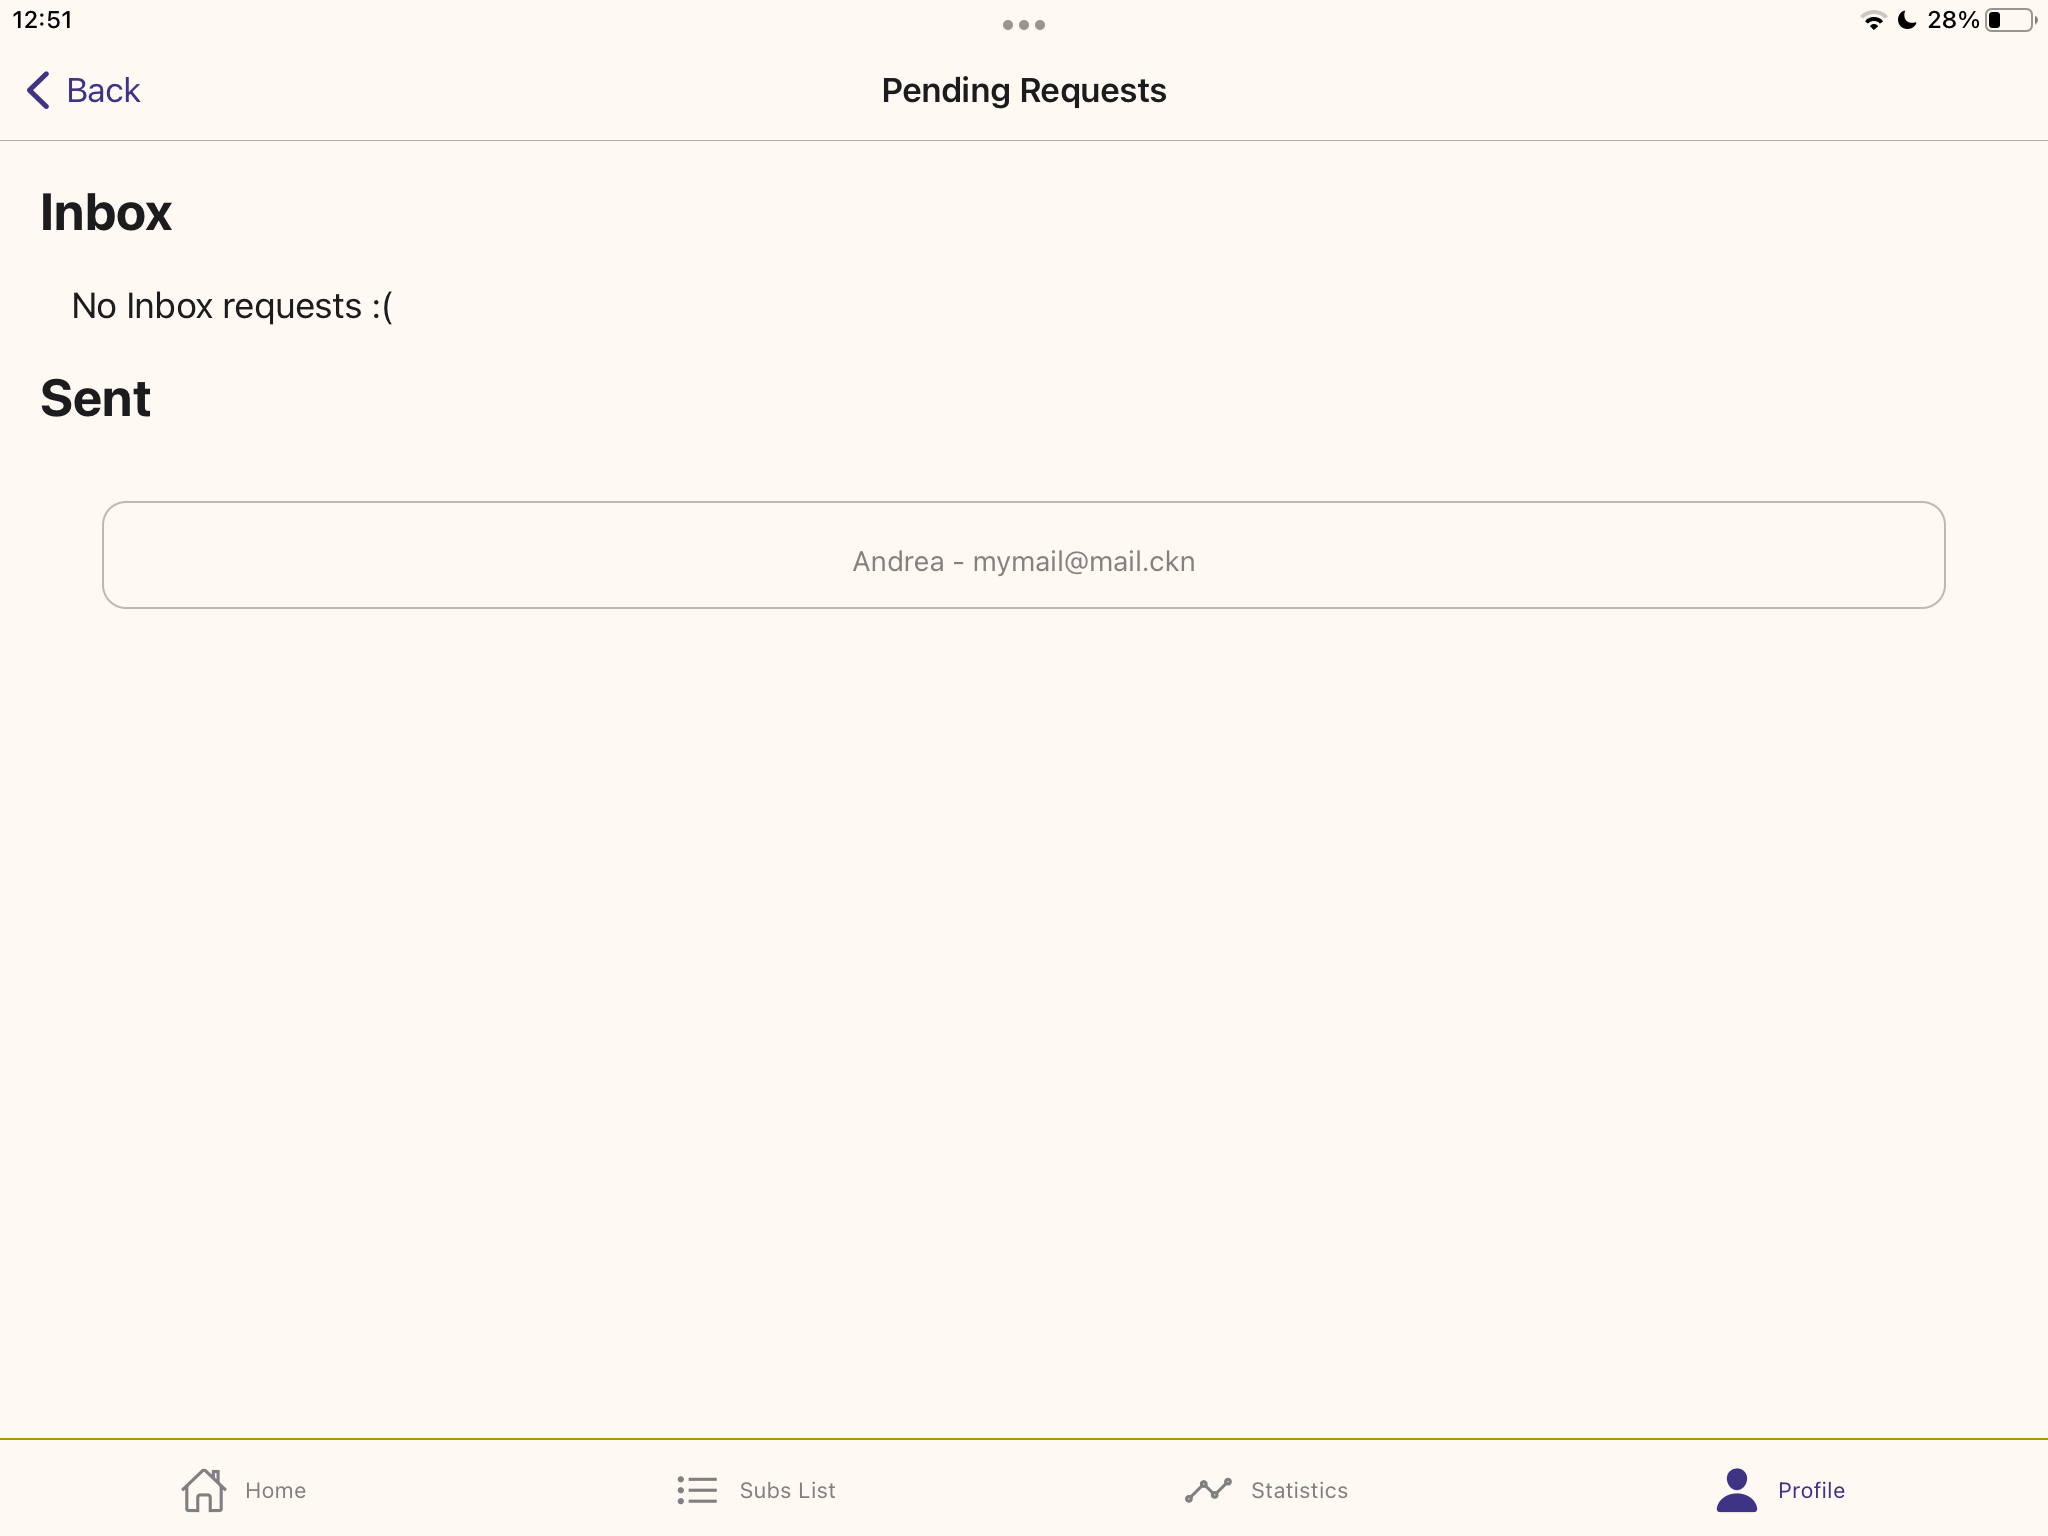
\includegraphics[width=0.7\textwidth, clip]{../../assets/tablet/inbox.PNG}
    \end{center}
    \caption{List of inbox and sent friends requests}
    \label{fig:tinbox}
\end{figure}

\begin{figure}[h!]
    \begin{center}
        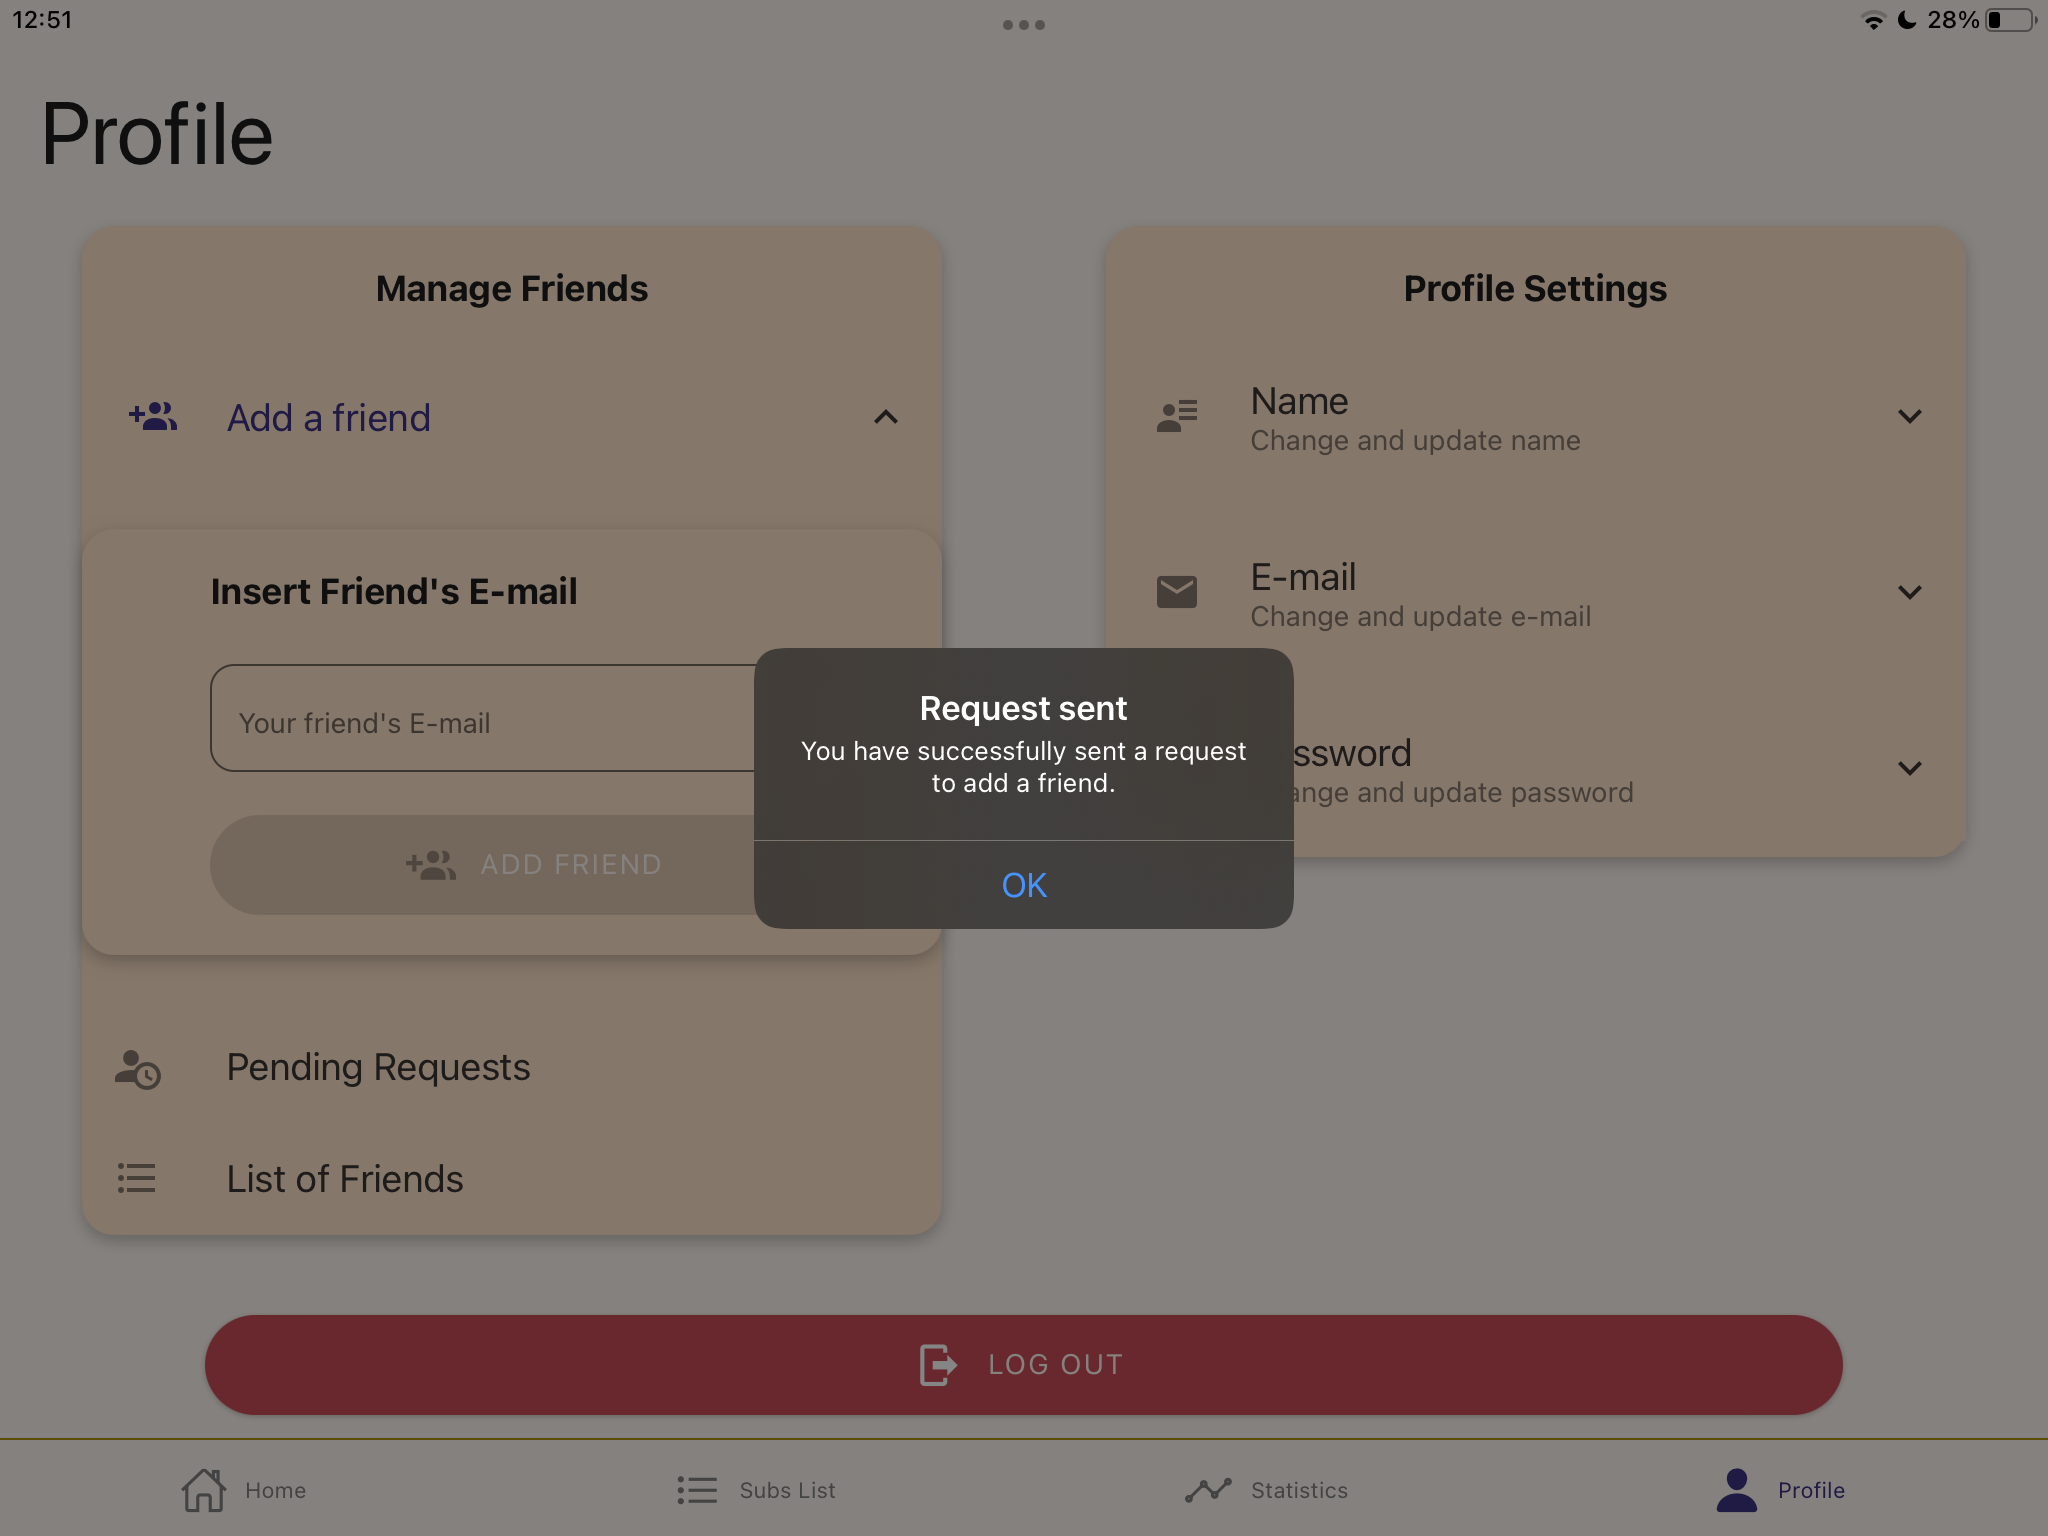
\includegraphics[width=0.7\textwidth, clip]{../../assets/tablet/alert.PNG}
    \end{center}
    \caption{Alert that notifies the user of a successful action}
    \label{fig:talert}
\end{figure}

\clearpage
\section{Implementation, Integration and Test Plan}\label{sec:test}
\subsection{Implementation Order}
The suggested implementation order should start from the frontend development and gradually link and implement the backend functions. This choice is dictated by the wish of knowing which information is needed and which will be displayed to the user. After following the design process and sketching many possible designs, it is important to choose the final application layout.

Once the design is decided, it is possible to code the frontend and then to finalize the implementation by understanding the kind and format of the information required by the frontend in order to work. Then the backend functions can be integrated smoothly into the design.

\subsection{Integration and Test Plan}
\subsubsection{Unit testing}
The framework employed for the application unit testing is \textbf{Jest}. In order to test the function correctness, we simulated server replies, formatted as JSON files.

We chose to start with the unit testing to verify the key functions of \textit{SubscribeME} in isolation. Great attention was given to undefined and null values as input, as they represent a big challenge for the correct functioning of the overall application.

\begin{figure}[h!]
    \begin{center}
        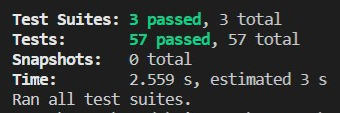
\includegraphics[width=0.4\textwidth, clip]{../../assets/test.png}
    \end{center}
    \caption{Test output}
    \label{fig:test}
\end{figure}

\textbf{Backend functions} and their interaction with the authenticator service provider and Cloud Firestore database have been tested through the \textbf{Firebase Local Emulator Suite}. This allows not to tamper with the production services and at the same time making sure to test every feature.

\subsubsection{Expo testing: simulator testing}
The application has been tested on \textbf{different operative systems} (both Android and iPhone) through the Expo Go application. The goal of the simulator testing is to find whether the code base responded in a proper manner to different renderings due to different operative systems. As expected, no big differences were shown in the experiment.

\subsubsection{On device testing}
Different \textbf{real-life devices} have been used to test the application, providing useful information regarding the visualization of data in different screen sizes.

Tablets and smartphones were used, both in portrait and in landscape mode. The different sizes were an issue at first, but finally the application was able to scale well.

\section{Future Development}\label{sec:dev}
Some possible improvements and further implementations could be:
\begin{itemize}
    \item a system of push \textbf{notifications} to alert the user even if the app is in background;
    \item \textbf{automatic recognition} of subscriptions from confirmation e-mails;
    \item \textbf{integrated payment} system;
    \item \textbf{chat} between friends.
\end{itemize}

\section{References}\label{sec:ref}
The tools that we used are:
\begin{itemize}
    \item \LaTeX\ for the document editing;
    \item \textit{starUML} for the use case diagram;
    \item \textit{draw.io} for the navigation tree diagram, the flow diagrams and the architecture diagram.
\end{itemize}
\end{document}